% ****************************************************************************************
\chapter{Konzeptionierung}
\label{chap:Konzeptionierung}
% ****************************************************************************************
Die grundlegenden Prinzipien und die daraus resultierenden Verfahren der Signalverarbeitung unter Verwendung von Mikrofonarrys sind ein essentieller Bestandteil dieser Arbeit. Es ist somit zwingend notwendig, die damit verbundenen mathematischen Zusammenhänge sowie die daraus abgeleiteten Methoden zu verstehen und gezielt einsetzen zu können.

Im folgenden Kapitel werden zunächst die elementaren Größen und Modelle der Array Signalverarbeitung eingeführt. Bezogen auf diese Grundlagen erfolgt anschließend der Entwurf eines mathematischen Modells zur Lösung der unter \Sec{sec:Problemformulierung} beschriebenen Problemstellung.

% ****************************************************************************************
\section{Grundlegende Annahmen und deren mathematische Zusammenhänge}
\label{sec:AnnahmenUndMatheZusammenhaenge}
% ****************************************************************************************
Im folgenden werden die System- sowie Signaleigenschaften des hier vorliegenden Systems untersucht. Die zu verarbeitenden Signale werden im weiteren Verlauf als Quellensignal und das von den Mikrofonen gelieferte als Sensorsignal bezeichnet.


% ****************************************************************************************
\subsection{System- und Signalmodell}
\label{subsec:Systemmodell}
% ****************************************************************************************
% Zunächst Beschreibung des SIMO - Systems mit Impulsantwort. Dann beschreiben, dass es sich um eine verzerrungsfreies System handelt da gilt y_n(t) = a_n * x_n(t-tau_n) (eigentlich entstehen nur lineare Verzerrungen, Dämpfung und Verzögerung)
% siehe script_ST1_v2.pdf Seite 40

\abb{IllustrationMikrofonarraySystems_a} illustriert den grundlegenden Aufbau eins Mikrofonarray Systems. Dieses besteht aus einem Quellensignal $s(k)$ sowie aus $N+1$ Sensorsignalen $y_n(k)$ die jeweils über eine der $N+1$ Kanalimpulsantworten $g_n$ mit dem Quellensignal verknüpft sind. Solch eine Signalkonstellation wird als SIMO\footnote{single-input multiple-output}-Modell \cite[S. 141]{Book_Array_Benesty} bezeichnet und kann durch folgende Gleichung beschrieben werden


\begin{equation}
\label{eq:SIMO}
    y_n(k) = g_{n} \ast s(k) + v_n(k)
\end{equation}

wobei $v_n(k)$ das dem Signal additiv überlagerte Umgebungsrauschen darstellt.


%\begin{align}
%        \mathbf{s}(k) & = \left[ s(k)~s(k-1) \cdots s(k-L_g+1)\right]^T \\
%        \mathbf{g}_N & = \left[ g_{N0}~g_{N1} \cdots g_{NL_g-1}\right]^T
%\end{align}


%Der Parameter $Lg$ steht dabei für die Länge der längsten Impulsantwort und $v(k)$ für das dem Signal additiv überlagerte Umgebungsrauschen.  



% ----------------------------------------- SUB-FIGURE -----------------------------------
\begin{figure}
        \centering
        \begin{subfigure}[b]{0.48\textwidth}
                \centering
                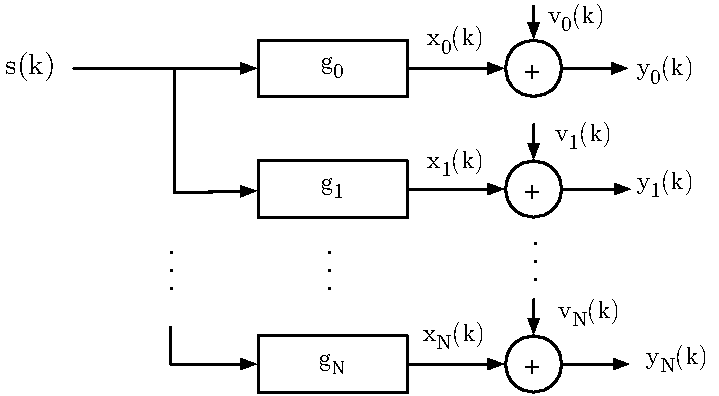
\includegraphics[width=\textwidth]{images/02_Konzeptionierung/IllustrationMikrofonarraySystem_a}
                \caption{}
                \label{fig:IllustrationMikrofonarraySystems_a}
        \end{subfigure}
        ~ %add desired spacing between images, e. g. ~, \quad, \qquad etc.
          %(or a blank line to force the subfigure onto a new line)
        \begin{subfigure}[b]{0.48\textwidth}
                \centering
                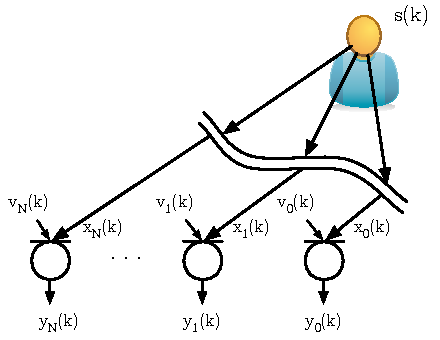
\includegraphics[width=\textwidth]{images/02_Konzeptionierung/IllustrationMikrofonarraySystem_b}
                \caption{}
                \label{fig:IllustrationMikrofonarraySystems_b}
        \end{subfigure}
        \caption{Illustration des Mikrofonarray Systems}
        %\caption{Verwendete Hardware}
\end{figure}
% ----------------------------------------- SUB-FIGURE -----------------------------------

Bei genauerer Untersuchung von \abb{IllustrationMikrofonarraySystems_b} können über die vom System verursachte Transformation des Quellensignals $s(k)$ in das Sensorsignal $y_n(k)$, unter Berücksichtigung von akustischen Freifeldbedingungen\footnote{ohne jegliche Reflexionen, nur der direkte Ausbeitungspfad wird betrachtet}, folgende Aussagen getroffen werden:


\begin{itemize}
    \item $s(k)$ wird durch die Entfernung von der Signalquelle zu den Sensoren um den Faktor $\alpha_n$ gedämpft/skaliert. Es gilt dabei: $0 \leq \alpha_n \leq 1$
    \item $s(k)$ wird durch die Entfernung zwischen der Signalquelle und den Mikrofonarray um eine Schallausbreitungszeit $T_S$ verzögert 
    \item $s(k)$ wird durch die Entfernung $d$ zwischen den einzelnen Sensoren um eine relative Zeit $\tau_{0n}$ verzögert. $\tau_{0n}$ bezieht sich dabei auf das Referenzmikrofon $M_0$.
     
\end{itemize}

Unter diesen Annahmen lässt sich $y_n(k)$ wie folgt ausdrücken

\begin{equation}
    y_n(k) = \alpha_n s(k - T_S- \tau_{n1}).
\end{equation}

%Bei $n=0$ folgt für die Laufzeiten $\tau_{n1} = 0$ und $T_n = t_S$.
Aus dieser Erkenntnis, dem in \Eq{SIMO} gezeigten Zusammenhang und der Vernachlässigung des additiven Rauschens $v(t)$ können die Kanalimpulsantworten $g_n$ wie folgt gefunden werden:

\begin{equation}
     \alpha_n s(k - T_S- \tau_{n0}) = \underbrace{\alpha_n \delta(k - T_S- \tau_{n0})}_{g_n} ~ \ast ~  s(k)
\end{equation}

Zur Ermittlung des Systemverhaltes ist es zwingend notwendig genaue Kenntnis über den Frequenz- und Phasengang zu erlangen. Diesen erhält man durch Fouriertransformation der $N+1$ Impulsantworten $g_n$.

\begin{equation}
g_n = \alpha_n \delta(k - T_S - \tau_{n1}) \hspace{0.5cm} \laplace \hspace{0.5cm} \underline{G}_n(\e^{\im \omega}) = \alpha_n \e^{-\im \omega (T_s + \tau_{n0})} \hspace{0.5cm} \text{für} \hspace{0.5cm} n=1 \dots N
\end{equation}


Der gewünschte Amplituden- und Phasengang lässt sich nun direkt aus dem komplexen Frequenzgang $\underline{G}_n(\e^{\im \omega})$ ablesen.



\begin{equation}
    \begin{array}{rrl}
  \text{\textbf{Amplitudengang:}} &
  \left | \underline{G}_n(\e^{\im \omega}) \right | & = \alpha_n \\
    \text{\textbf{Phasengang:}} &
    \varphi_n(f) & = - 2 \pi f (T_s + \tau_{n0})
   \end{array}
  \label{eq:SystemEigenschaften}
\end{equation}
 

Aus dem Frequenzgang leitet sich ein konstanter Amplitudengang $\alpha_n$ (Dämpfungsverzerrung) sowie ein frequenzproportionaler Phasengang (Phasenverzerrung) $-2 \pi f  (T_s + \tau_{n0}) \sim f$ ab. Diese Systemeigenschaft lässt sich direkt einem idealen verzerrungsfreien LTI\footnote{Linear Time Invariant}-System zuordnen \cite[S. 63ff]{Book_SignalTransmission_Kammayer}. Das hier zu implementierende reale System muss das in \Eq{SystemEigenschaften} dargestellte Verhalten innerhalb der Signalbandbreite möglichst gut approximieren.




% ****************************************************************************************
%\subsection{Signalmodell}
%\label{Subsec:Signalmodell}
% ****************************************************************************************
%\todo[inline]{Beschreibung des Signalmodels wie im Buch von Benisty
%sowie Einführung der Variablen,Single-Source reverberant model, MIMO-System}
%\missingfigure{Ein erklärendes Bild zum Signalmodel - Sprecher, Sensoren, Echo, Rauschen \dots}

% ****************************************************************************************
\subsection{Sensormodell}
\label{subsec:Sensormodell}
% ****************************************************************************************

% ****************************************************************************************
\subsubsection{Lineares zweidimensionales Sensorarray}
\label{subsubsec:linearesArray}
% ****************************************************************************************
\abb{SensormodellLinearenArrays} zeigt den Aufbau eines linearen äquidistanten Mikrofonarrays (ULA\footnote{Uniform Linear Array}) mit einer Anzahl von $N+1$ Sensoren und dem Sensorabstand $d$. Bei einer solchen Anordnung legen die Schallwellen, abhängig vom Schalleinfallswinkel $\theta$ unterschiedlich lange Wege von der Signalquelle zu den einzelnen Sensoren zurück. Unter Berücksichtigung einer ebenen Wellenfront sowie einer bekannten Arraygeometrie lässt sich mit Hilfe der Laufzeitdifferenz $\tau_{ULA}$ und der Schallgeschwindigkeit\footnote{Approximierte Geschwindigkeit bei einer Raumtemperatur von 20°C} $c \approx 343 \frac{m}{s}$ folgender Zusammenhang definieren

\begin{equation}\label{eq:ULA_1}
    \tau_{ULA}= \frac{d}{c} \cdot \cos(\theta)
\end{equation}

Für den hier beschriebenen Fall kann die Laufzeitdifferenz zwischen Referenzsensor $M_0$ und Sensor $M_N$ durch die lineare Funktion $f_{0n,ULA}(\tau)$ ausgedrückt werden


\begin{equation}\label{eq:ULA_2}
    f_{0n,ULA}(\tau) = n \cdot \tau_{ULA} \eqspace \text{mit} \eqspace n=1,2, \dots N
\end{equation}


%Zur Berechnung der Laufzeitdifferenzen zwischen allen Sensorpaarkombinationen $M_{01}, M_{02}, \dots, M_{0N},M_{12}, M_{13} \dots,  M_{(N-1)N}$ kann ebenfalls der lineare Zusammenhang aus \Eq{ULA_2} genutzt werden. Bei einer Anzahl von $N$ Sensoren ergeben sich somit $\frac{N+1}{2} \cdot N$ Laufzeiten.



\myFigure{real}                                      % Figure tag (missing, real)
         {big}                                       % Size (small,medium,big)
         {h}                                         % z.B. htbp
         {Sensormodell eines linearen Arrays}        % Figure title
         {SensormodellLinearenArrays}                % Figure label 
         {02_Konzeptionierung/ULA}                   % Path to real figure
         

% ****************************************************************************************
\subsubsection{Dreidimensionales Sensorarray}
\label{subsubsec:3DArray}
% ****************************************************************************************
Zur räumlichen Detektion einer Schallquelle ist es notwendig eine Sensorgeometrie zu finden, in der die Richtungsinformation durch den Azimuthwinkel $\theta$ sowie den Elevationswinkel $\phi$ ausgedrückt werden kann. Eine solches Array lässt sich mit Hilfe einer Matrix $\mathbf{M}$ repräsentieren, wobei jede Spalte die Position eines der $N+1$ Sensoren in einem dreidimensionalen euklidschen Raum beschreibt. 

\begin{equation}
    \mathbf{M}_{3 \times N+1} = 
    \begin{bmatrix}
        m_{x_0} & m_{x_1} & \dots & m_{x_N} \\
        m_{y_0} & m_{y_1} & \dots & m_{y_N} \\
        m_{z_0} & m_{z_1} & \dots & m_{z_N} \\
    \end{bmatrix}
\end{equation}



%Die erste Spalte dieser Matrix stellt dann den Referenzsensor dar und kann als Zentrum dieses dreidimesionalen Raums betrachtet werden.
\abb{3D_Array_Prinzip_1} zeigt den Referenzsensor im Zentrum dieses Raumes mit einem aus einer beliebigen Richtung eintreffenden Signal. Dieses Signal kann über den Einheitsvektor $\mathbf{s}$, welcher senkrecht zur von der Quelle Emittierten ebenen Wellenfront steht, beschrieben werden. Im Hinblick auf eine spätere Extraktion der oben genannten Raumwinkel wird $\mathbf{s}$ in Kugelkoordinaten ausgedrückt.

\begin{equation}
\textbf{s}_{3 \times 1} =
\begin{bmatrix}
        s_x \\
        s_y \\
        s_z\\
    \end{bmatrix}
    =
    \begin{bmatrix}
        \cos{(\phi)} \cos{(\theta)} \\
        \cos{(\phi)} \sin{(\theta)} \\
        \sin{(\phi)}\\
    \end{bmatrix}
\end{equation}

Der Azimuthwinkel kann dabei die Werte $0° \leq \theta < 360°$ und der Elevationswinkel $-90° \leq \phi \leq 90°$ annehmen.


\myFigure{real} % Figure tag (missing, real)
         {small} % Size (small,medium,big)
         {h} % z.B. htbp
         {Beschreibung der Signalquelle im Raum unter Verwendung von Azimuth- und Elevationswinkel.} % Figure title
         {3D_Array_Prinzip_1} % Figure label 
         {02_Konzeptionierung/3D_Array_Prinzip_1}


Als nächster Designschritt folgt der Zusammenhang zwischen dem Schalleinfallswinkeln und der Laufzeitdifferenz der einzelnen Sensorpaare. \abb{3D_Array_Prinzip_2} illustriert ein Sensorpaar, das durch die Spaltenvektoren $\mathbf{m_0}$ und $\mathbf{m_1}$ repräsentiert wird. Der Verbindungsvektor $\mathbf{m_{01}}$ zwischen den Sensoren berechnet sich mit $\mathbf{m_1} - \mathbf{m_0}$.
% und der Einheitsvektor $\mathbf{s}$ kann erneut als die Schalleinfallsrichtung aufgefasst werden. 
Zu beachten ist, dass $\mathbf{s}$ nun in Richtung der Sensoren zeigt und somit gilt $\mathbf{s} = -\left[\cos(\phi) \cos(\theta) ~  \cos(\phi) \sin(\theta) ~ \sin(\phi) \right]^T$. Die zusätzliche Distanz, die der Schall zurücklegen muss, um von Sensor $M_0$ zu $M_1$ zu gelangen wird als Laufwegunterschied $s_{01}$ bezeichnet. Wie in \abb{3D_Array_Prinzip_2} dargestellt ergibt sich $s_{01}$ durch Projektion von $\mathbf{m_{01}}$ mit Bezug auf den Schalleinfallsvektor $\mathbf{s}$.  $s_{01}$ kann somit durch das Skalarprodukt 

\begin{equation}
    s_{01} = \left ( \mathbf{m_1} - \mathbf{m_0} \right )^T \mathbf{s} = \mathbf{m_{01}}^T \, \mathbf{s}
\end{equation}

ermittelt werden. Folglich bildet sich die Laufzeitdifferenz $\tau_{01}$ durch

\begin{equation}
    \tau_{01} = \left[ \mathbf{m_{01}}^T \, \mathbf{s} \right] \cdot c^{-1}
\end{equation}
  
%% ALT
%Zur Bestimmung der Laufzeitdifferenzen zwischen allen $N$ Sensoren muss zunächst eine Matrix $\mathbf{A}$ definiert werden, in der die Verbindungsvektoren $\mathbf{m}$ aller $M = \frac{N}{2} \cdot (N-1)$ Sensorpaarkombinationen definiert sind.

%\begin{equation}
%    \mathbf{A}_{3 \times M} = 
%    \begin{bmatrix}
%        \mathbf{m}_{12} & \mathbf{m}_{13} & \dots & \mathbf{m}_{1N} & \mathbf{m}_{23} & \mathbf{m}_{24} & \dots & \mathbf{m}_{(N-1)N}
%    \end{bmatrix}
%%    =
%%    \begin{bmatrix}
%%        m_{x_{12}} & m_{x_{13}} & \dots & m_{x_{(N-1)N}} \\
%%        m_{y_{12}} & m_{y_{13}} & \dots & m_{y_{(N-1)N}} \\
%%        m_{z_{12}} & m_{z_{13}} & \dots & m_{z_{(N-1)N}}
%%    \end{bmatrix}
%\end{equation}


Zur Bestimmung der Laufzeitdifferenzen zwischen allen Sensoren muss zunächst eine Matrix $\mathbf{A}$ definiert werden, in der die Verbindungsvektoren $\mathbf{m_{0n}}$ aller $N$ Sensorpaarkombinationen definiert sind.

\begin{equation}
    \mathbf{A}_{3 \times N} = 
    \begin{bmatrix}
        \mathbf{m}_{01} & \mathbf{m}_{02} & \dots & \mathbf{m}_{0N}    \end{bmatrix}
%    =
%    \begin{bmatrix}
%        m_{x_{12}} & m_{x_{13}} & \dots & m_{x_{(N-1)N}} \\
%        m_{y_{12}} & m_{y_{13}} & \dots & m_{y_{(N-1)N}} \\
%        m_{z_{12}} & m_{z_{13}} & \dots & m_{z_{(N-1)N}}
%    \end{bmatrix}
\end{equation}



Dabei gilt für $\mathbf{m}_{3 \times 1}$ der Ausdruck

\begin{equation}
    \mathbf{m}_{1N} = 
    \begin{bmatrix}
       x_{0N} \\
       y_{0N} \\
       z_{0N}
    \end{bmatrix}
    =
    \begin{bmatrix}
       x_{N} - x_0 \\
       y_{N} - y_0 \\
       z_{N} - z_0
    \end{bmatrix}
\end{equation}

Die gesuchten Laufzeitdifferenzen können nun in einem Vektor $\boldsymbol{\tau}_{N \times 1}$ beschrieben werden. Für ein statisches Sensorarray sind diese ausschließlich von der Schalleinfallsrichtung und damit von den Winkeln $\phi$ und $\theta$ abhängig.

\begin{equation}\label{eq:DOA_winkel}
    \begin{array}{ll}
        \boldsymbol{\tau}(\phi, \theta)_{N \times 1} & =  \left[ \left( \mathbf{A}^T \right)_{N \times 3} \cdot \mathbf{s}_{3 \times 1} \right]_{N \times 1} \cdot c^{-1} \\
                                                     & = f_n(\phi, \theta) \eqspace \text{mit} \eqspace n = 1,2, \dots, N
    \end{array}
\end{equation}

Ein Sensorarray mit beliebiger Geometrie kann so analog zu \Eq{ULA_2} durch die nicht-lineare Funktion $f_n(\phi, \theta)$ beschrieben werden. Auf Grund einer nicht-quadratischen Matrix $\mathbf{A}$ muss dessen Inverse als Pseudoinverse $\textbf{A}^{+}$ gebildet werden \cite[S. 185]{Book_MatrixTheory_Piziak}. \Eq{DOA_winkel} kann so mit Bezug auf $\boldsymbol{s}$ in

\begin{equation}
        \boldsymbol{\hat s}(\phi, \theta)_{3 \times 1} = \left \{ \left [ \underbrace{\left( \textbf{A} \cdot \textbf{A}^T \right)^{-1} \cdot \textbf{A}}_{\textbf{A}^{+}}  \right]_{3 \times N} \cdot \boldsymbol{\hat \tau}(\phi, \theta)_{N \times 1} \right \}_{3 \times 1} \cdot c  
\end{equation}

umgeformt werden. $\boldsymbol{\hat s}(\phi, \theta)$ beschreibt dabei den geschätzten Normalvektor\footnote{$\boldsymbol{s}$ steht senkrecht zur einlaufenden Wellenfront} zur Schalleinfallsrichtung und $\boldsymbol{\hat \tau}$ die Schätzung der paarweisen Laufzeitdifferenz \cite[S. 71]{Master_Array_Varma}.
 
 
 
\subsubsection{Räumliches Aliasing} 
Basierend auf den Ausführungen zum räumlichen Alias-Effekt in \cite[8 f]{Master_Array_Pikora} ist bei der Dimensionierung des Sensorarrays folgendes Kriterium zu berücksichtigen:
 \begin{equation}\label{eq:raemlichesAliasing}
     d_{min} \leq \frac{\lambda}{2} = \frac{c}{2 f_{max}}
 \end{equation}

 $d_{min}$ ist dabei die geringste Distanz zwischen zwei Sensoren und $f_{max}$ die größte im Signal enthaltene Frequenz.
 
%\todo[inline]{................................................................................................................................}

\myFigure{real} % Figure tag (missing, real)
         {medium} % Size (small,medium,big)
         {h} % z.B. htbp
         {Laufwegdifferenz als Projektionsvetor zwischen zwei Sensoren im Bezug auf den Schalleinfallsvektor $\mathbf{s}$} % Figure title
         {3D_Array_Prinzip_2} % Figure label 
         {02_Konzeptionierung/3D_Array_Prinzip_2}






% ****************************************************************************************        
\subsubsection{Akustisches Fernfeld}
\label{subsubsec:Fernfeld}
% ****************************************************************************************
Zur Sicherstellung einer ebenen Wellenfront muss sich die Signalquelle wie in \abb{MikrofonarrayFernfeld} dargestellt, im akustischen Fernfeld befinden. Unter diesen Umständen darf die von der Quelle emittierte Kugelwelle $s(k)$ auf einem kleinen Bereich linear approximiert werden. Für die Entfernung $r$, von Array bis zu dem Punkt, an dem die Fernfeldbedingung angenommen werden kann muss folgendes gelten\cite[S. 36f]{Book_Audio_Goerne}:

\begin{equation}
    k \cdot r >> 1 \eqspace \text{mit} \eqspace k = \frac{2 \pi}{\lambda} = \frac{2\pi f}{c}
\end{equation}


%\begin{equation}\label{eq:Fernfeld}
%    \hat d _D = \frac{\hat d}{D} = \frac{\kappa}{16\pi} \cdot kD = \frac{\kappa}{8} \cdot \frac{f}{c} \cdot D
%\end{equation}
%
%$\hat d$ beschreibt dabei die Distanz von Signalquelle zu Mikrofonarray, $D$ die größte im Array vorkommende Entfernung zwischen zwei Sensoren und $k$ die Kreiswellenzahl mit
%
%\begin{equation}\label{eq:Kreiswellenzahl}
%    k = \frac{2 \pi}{\lambda} \hspace{0.5cm} \text{und} \hspace{0.5cm} \lambda = \frac{c}{f}
%\end{equation}


\myFigure{real}                  % Figure tag (missing, real)
         {big}                 % Size (small,medium,big)
         {h!}             % z.B. htbp
         {Mikrofonarray im akustischen Fernfeld}                % Figure title
         {MikrofonarrayFernfeld}                % Figure label 
         {02_Konzeptionierung/Fernfeld}     % Path to real figure











%\todo[inline]{Geometrie, Wellenausbreitung (ebene Welle, Fernfeld),
%Koordinatensystem,Mikrofonvektoren, Entwicklung 3D-Arrays wie in
%\texttt{chap2-MIC.pdf}}
%\missingfigure{Ein erklärendes Bild zum Mikrofonmodel, Koordinatensystem,
%Projektion der DOA durch ebene Welle}


% ****************************************************************************************
\section{Schätzverfahren}
\label{sec:Schaetzverfahren}
% ****************************************************************************************
In \Sec{subsec:Sensormodell} wurde gezeigt, dass die Laufzeitdifferenz $\tau$ zwischen den einzelnen Sensorpaaren genutzt werden kann, um mit Hilfe geometrischer Zusammenhänge die Schalleinfallsrichtung zu bestimmen. Da $\tau$ ein unbekannter Parameter ist, kann dieser mit Hilfe geeigneter Verfahren aus mindestens zwei Sensorsignalen geschätzt werden.
Aufgrund der unter \Sec{subsec:Systemmodell} abgeleiteten Systemeigenschaften wie der Verzögerung und Skalierung des Quellensignals durch die Sensorgeometrie kann hier die Kreuzkorrelation als Schätzverfahren angewandt werden.

% ****************************************************************************************
\subsection{Kreuzkorrelation}
\label{subsec:Kreuzkorrelation}
% ****************************************************************************************
Die Kreuzkorrelation zweier kontinuierlicher Funktionen $x(t)$ und $y(t)$ über einem Intervall $T$ ist definiert mit

\begin{equation}\label{eq:kreuzkorrelation}
    r_{xy}(\tau) = \lim_{T \to \infty} \, \frac{1}{T} \int_{0}^{T} x(t) \cdot y(t+\tau) \, \mathrm{d}t
\end{equation}

Die Eigenschaften dieser Schätzmethode lassen sich im Bezug auf die hier vorliegenden Signale anhand eines anschaulichem Beispiels erläutern. Wie in \abb{Kreuzkorrelation_Prinzip} dargestellt sei $x(t)$ ein Rechteckimpuls der Pulsbreite $T_p$ und $y(t) = \alpha \cdot x(t-\Delta t)$ eine um $\alpha$ skalierte sowie um $\Delta t$ verzögerte Version von $x(t)$. Als Ergebnis der Kreuzkorrelation ergibt sich ein Dreieckimpuls der doppelten Pulsbreite. Dieser ist um die Verzögerungszeit $\Delta t$ zentriert und hat den Spitzenwert $\alpha \cdot T_p$. In Anbetracht einer realen Implementierung ist die in \Eq{kreuzkorrelation} dargestellte Grenzwertbildung nicht möglich. Die Korrelation kann so nur über einem endlichen Intervall $T<\infty$ stattfinden was zu eine Schätzung $\Delta \hat t$ der Laufzeitverzögerung $ \Delta t$ durch


\begin{equation}\label{eq:kreuzkorrelationMax}
    \Delta \hat t = \arg \max_{\tau} \left[ \hat r_{xy}(\tau) \right ]
\end{equation}

führt. Zu erkennen ist, dass diese Methode eine Funktion liefert, die eine Aussage über die Ähnlichkeit der korrelierten Signale macht. An der Stelle, an der sich beide Funktionen am meisten ähneln, besitzt die Kreuzkorrelationsfunktion $\hat r_{xy}(\tau)$ ihr Maximum. Zu beachten ist, dass beide Signale frei von jeglichem Gleichanteil sind. Wird diese Bedingung verletzt, besitzt $\hat r_{xy}(\tau)$ ihren Maximalwert stets bei $\tau=0$.

Da die hier zu verarbeitenden Signale in diskreter Form vorliegen, muss das Korrelationsintegral in eine Korrelationssumme der Fensterlänge $K$ umgeformt werden. Unter der Bedingung $N<\infty$ folgt die geschätzte Kreuzkorrelationsfolge $\hat r_{xy}[k]$ der Länge $2K-1$ durch

\begin{equation}\label{eq:kreuzkorrelationDiskret}
    \hat r_{xy}[k] = \frac{1}{K} \, \sum_{n=0}^{K-1} x[n] \cdot y[n+k] \eqspace \text{mit} \eqspace -(K-1) \leq k \leq K-1
\end{equation}

Zu berücksichtigen ist dabei allerdings, dass nur Abtastwerte aus dem Beobachtungsintervall $0 \leq n \leq K-1$ zur Verfügung stehen. Wird beispielsweise nach \Eq{kreuzkorrelationDiskret} $\hat r_{xy}[k]$ für den Verschiebezeitpunkt $k=5$ und einer Fensterlänge $K=10$ berechnet, wird auf den Wert $x[14]$ der Musterfunktion zugegriffen. Dieser Abtastwert existiert jedoch nicht. Die Summationsgrenzen sind daher zu modifizieren \cite[S. 321 ff]{Book_SignalProcessing_Kammayer}. Es folgt:

\begin{equation}\label{eq:kreuzkorrelationDiskretMod}
    \hat r_{xy}[k]=\begin{cases}
        \frac{1}{K} \, \sum_{n=0}^{K-1-k} x[n] \cdot y[n+k]  & \text{für } 0 \leq k \leq K-1 \\
      \frac{1}{K} \, \sum_{n=-k}^{K-1} x[n] \cdot y[n+k] & \text{für } -(K-1) \leq k < 0 \\
      0 & \text{sonst}
    \end{cases}
\end{equation}

Bei Betrachtung von \Eq{kreuzkorrelationDiskret} im Hinblick auf den aufzuwendenden Rechenaufwand fällt auf, dass diverse Additions- sowie Multiplikationsoperationen durchzuführen sind. Zur Korrelation von zwei  Datenfolgen der Länge $K$ müssen $(2K-1) \cdot (K-1)$ Additionen sowie $(2K-1) \cdot K$ Multiplikationen ausgeführt werden. Der Rechenaufwand wächst somit quadratisch mit wachsender Fensterlänge $K$, wodurch sich diese Rechenmethode für eine zeitkritische Implementierung als ungeeignet erweist.


\myFigure{real}                  % Figure tag (missing, real)
         {small}                 % Size (small,medium,big)
         {h!}             % z.B. htbp
         {Kreuzkorrelation zwischen $x(t)$ und $y(t)$. Die Funktion $y(t)$ ist dabei eine skalierte und verzögerte Version von $x(t)$.}                % Figure title
         {Kreuzkorrelation_Prinzip}                % Figure label 
         {02_Konzeptionierung/Kreuzkorrelation_Prinzip}     % Path to real figure



% ****************************************************************************************
\subsubsection{Schnelle Kreuzkorrelation}
\label{subsubsec:SchnelleKreuzkorrelatio}
% ****************************************************************************************
Im Hinblick auf eine spätere Echtzeitimplementierung ist eine effiziente Methode zur Berechnung der Kreuzkorrelation von großem Interesse. Es kann gezeigt werden, dass dies über eine Umformung der Korrelationssumme in eine Faltungssummer erreicht werden kann. 
Aufgrund des hier vorliegenden LTI-Systems kann dessen Ausgangsfolge $g[n]$ durch die Faltung zwischen einer Eingangsfolge $s[n]$ und der Systemimpulsantwortfolge $h[n]$ definiert werden:

\begin{align}\label{eq:faltungDiskret}
        g[n] & = s[n] \ast h[n] \nonumber \\
             & = \sum_{k = -\infty}^{\infty} s[k] \cdot h[n-k]
\end{align}


Ein Vergleich von \Eq{kreuzkorrelationDiskret} und \Eq{faltungDiskret} ergibt, dass lediglich die Summationsvariablen vertauscht sind. Als erster Umformungsschritt erfolgt so zunächst eine Anpassung der Indizes von $y$

\begin{equation}
 \hat r_{xy}[k] = \frac{1}{K} \, \sum_{n=0}^{K-1-k} x[n] \cdot y[k-(-n)] \eqspace \text{für} \eqspace 0 \leq k \leq K-1
\end{equation}

Des weiteren wird $x[n]$ in $x[-(-n)]$ umgeformt, womit folgt

\begin{equation}
 \hat r_{xy}[k] = \frac{1}{K} \, \sum_{n=0}^{K-1-k} x[-(-n)] \cdot y[k-(-n)] \eqspace \text{für} \eqspace 0 \leq k \leq K-1
\end{equation}

Unter Nutzung von \Eq{faltungDiskret} kann die Kreuzkorrelierte $\hat r_{xy}[k]$ als Faltungsoperation ausgedrückt werden

\begin{equation}
    \hat r_{xy}[k] = x[-n] \ast y[n]
\end{equation}

Zur Rechenzeitoptimierung kann nun unter Berücksichtigung folgender Korrespondenz

\begin{align}
    \hat r_{xy}[k] \eqspace \laplace \eqspace \underline{R}_{xy}[l] = & \underline{X}[-l] \cdot \underline{Y}[l] \\
    = & \underline{X}[l]^{*} \cdot \underline{Y}[l]
\end{align}

auf die FFT\footnote{Fast Fourier-Transformation}, einer schnellen Variante der diskreten Fourier Transformation (DFT\footnote{Diskrete Fourier-Transformation}) und deren Inversen (IDFT\footnote{Inverse Diskrete Fourier-Transformation}) zurückgegriffen werden. $\underline{R}_{xy}[l]$ beschreibt dabei das Kreuzleistungsdichtespektrum. Eine effiziente Variante der geschätzten Kreuzkorrelationsfunktion $\hat r_{xy}[k]$ kann so wie folgt als schnelle Kreuzkorrelation errechnet werden:

\begin{equation}
    \hat r_{xy}[k] = \mathrm{IDFT} \left \{ \left ( \mathrm{DFT}\{ x[n] \}\right )^* \cdot  \mathrm{DFT}\{ y[n] \} \right \}
\end{equation}


Zur Anwendung diese Verfahrens müssen zwei Bedingungen in Bezug auf die Eigenschaften von DFT \bzw FFT erfüllt sein:

\begin{enumerate}
    \item\label{itm:fftBedingung} Die DFT-Länge K muss auf Grund der hier verwendeten Radix-2-FFT einer Zweierpotenz mit $K = 2^p$ und $p \in  \mathbb{N}^{+}$ entsprechen. Diese Form der FFT zerlegt die herkömmliche DFT sukzessiv in zwei DFT der halben Länge, bis schließlich eine Transformationslänge zwei erreicht wird \cite[S. 222 ff]{Book_SigSys_Werner}.
    
     \item Um einen Überfaltungsfehler zu vermeiden, müssen den Datenfolgen $x[n]$ und $y[n]$ der Länge $K$ vor der Transformation in den Frequenzbereich mindestens $K-1$ Nullen angehängt werden (Zeropadding) \cite[S. 215 ff]{Book_SigSys_Werner}. Auf Grund der Bedingung aus Punkt \ref{itm:fftBedingung} wird die Datenfolge um eine weitere Null auf die Länge $2K$ verlängert. Der zusätzliche Ergebniswert befindet sich an der ersten Stelle $\hat r_{xy}[0] = 0$ und kann ignoriert werden.
     
     
     \item Nach der Rücktransformation in den Zeitbereich muss die gesamte Funktion $\hat r_{xy}[k]$ um dessen halbe Länge auf der Zeitachse nach rechts verschoben werden. Die Zeitkomponente $k=0$ befindet sich dann im Zentrum des Koordinatensystems, wodurch negative sowie positive Verzögerungen abgelesen werden können. Dies kann \zB in \matlab mit der eingebetteten Funktion \texttt{fftshift()} erreicht werden.
\end{enumerate}


			
% ****************************************************************************************
\subsubsection{Erwartungstreue Schätzung}
\label{subsubsec:ErwartungstreueSchaetzung}
% ****************************************************************************************
Wie bereits im vorangegangenen Abschnitt erwähnt, wird eine Korrelation über einen endlich langen Signalabschnitt berechnet. Da die Eingabedaten in einem kontinuierlichen Datenstrom vorliegen, muss diesem eine gewisse Menge an Werten entnommen und anschließend verarbeitet werden. Betrachtet man diese Datenentnahme im Hinblick auf eine Fensterfunktion, entspricht dies einer Multiplikation des Datenstroms mit einem Rechteckfenster wie bereits in \abb{Kreuzkorrelation_Prinzip} illustriert. Diese Fenstermethode weist folgende spektrale Eigenschaften auf (\vgl \cite[S. 301]{Book_SignalProcessing_Kammayer}):


\begin{align}
        \hat r_{xy}(t) & = s_1(t) \cdot \frac{1}{T} \, \mathrm{rect}\left(\frac{t}{T}\right) \ast s_2(t) \cdot \frac{1}{T} \, \mathrm{rect}\left(\frac{t}{T}\right) \\
                 & = \mathscr{F} \left\{ s_1(t) \cdot \frac{1}{T} \, \mathrm{rect}\left(\frac{t}{T}\right) \ast s_2(t) \cdot \frac{1}{T} \, \mathrm{rect}\left(\frac{t}{T}\right) \right \}\\
                 & = \underline{S_1}(f) \ast \mathrm{si}\left(\pi f T\right) \cdot \underline{S_2}(f) \ast \mathrm{si}\left(\pi f T\right)\\
                 & =  \underline{S_1}(f) \cdot  \underline{S_2}(f) \ast \mathrm{si}^2\left(\pi f T\right) \\
                 & = s_1(t) \ast s_2(t) \cdot \frac{1}{T} \, \mathrm{tri}\left(\frac{t}{T}\right)
\end{align}


Die Entnahme von Daten mit einem rechteckförmigen Fenster bewirkt im Faltungs-/Korrelationsergebnis eine Gewichtung durch ein dreieckförmiges Fenster (Barlett-Fenster). Man beschreibt ein solches Vorgehen als nicht-erwartungstreu. Die Aussagekraft der Korrelationswerte sinkt linear mit steigender Entfernung zur Korrelogrammmitte. Um aus diesem Ergebnis eine erwartungstreue Schätzung zu erhalten, ist die gesamte Folge mit der Umkehrfunktion des Dreieckfensters zu gewichten. Wie sich später noch zeigen wird, ist diese Ausgleichsoperation bei der hier implementierten Anwendung nicht notwendig. 


% ****************************************************************************************
\subsection{Mehrkanal-Kreuzkorrelationskoeffizient (MCCC)}
\label{subsec:MehrkanalKreuzkorrelationskoeffizient}
% ****************************************************************************************
Das unter \Sec{subsec:Kreuzkorrelation} eingeführte Schätzverfahren ist lediglich in der Lage, Aussagen über die Korrelation zweier Signale zu geben. Zur Verarbeitung von $N+1$ Signalen bedarf es einer Erweiterung dieser Methode \cite[S. 196ff]{Book_Array_Benesty}, \cite{Paper_Array_Benesty}. 

Die grundsätzliche Idee der Verwendung von Arrays mit mehr als zwei Sensoren ist das hohe Maß an redundanter Information. Diese kann extrahiert und zur Erhöhung der Systemrobustheit in realer akustischer Umgebung (\zB stark hallender Raum, additiv überlagerte Störungen durch Umgebungsgeräusche) genutzt werden. Nutzt man die in \Sec{subsec:Sensormodell} beschriebenen Zusammenhänge, kann die Richtcharakteristik des Arrays in eine gewünschte Schalleinfallsrichtung geschwenkt werden. Im Umkehrschluss kann dann den Laufzeitverzögerungen zwischen den einzelnen Sensorpaaren insgesamt genau eine Schalleinfallsrichting zugeordnet werden. Um die letztere Eigenschaft auszunutzen, wird zunächst ein Signalvektor der From

\begin{equation}\label{eq:DOA_SigVec}
    \mathbf{y}_{\phi,\theta}(k) = \left [ y_0(k) \eqspace y_1 [k + f_1(\phi, \theta) ] \eqspace \dots \eqspace y_N[k+f_N(\phi, \theta) ] \right ]^T
\end{equation}

definiert. $F_n(\phi, \theta)$ beschreibt dabei die in \Eq{DOA_winkel} beschriebenen Verzögerungen, mit denen die Sensorsignale zeitlich zueinander ausgerichtet werden. Unter Angabe eines angenommenen Azimuth- und Elevationswinkels kann so der Array-Beobachtungsvektor $\mathbf{y}_{\phi,\theta}[k]$ beliebig im Raum  ausgerichtet werden. Zur Nutzung der unter \Eq{DOA_SigVec} genannten Laufzeitbeziehungen erfolgt nun die Berechnung der räumlichen Korrelationsmatrix $\mathbf{R}_{\phi,\theta}$. Diese beschreibt die Signalleistung zwischen den einzelnen Sensorsignalen und wird auch als Kovarianzmatrix bezeichnet. 



%\begin{align}
%\mathbf{R}_{\phi,\theta} & = \mathrm{E} \left \{ \mathbf{y}_{\phi,\theta}[k] \, \mathbf{y}^T_{\phi,\theta}[k]  \right \} \\
%                & = 
%    \begin{bmatrix}
%    \sigma_{y_1}^2	     & r_{a,y_1 y_2}(p)     & \dots & r_{a,y_1 y_N}(p)      \\
%    r_{a,y_2 y_1}(p)	  & \sigma_{y_2}^2      & \dots & r_{a,y_2 y_N}(p)       \\
%    \vdots	            & \vdots 	           & \ddots & \vdots                \\
%    r_{a,y_N y_1}(p) 	  & r_{a,y_N y_2}(p)     & \dots	 & \sigma_{y_N}^2
%    \end{bmatrix}
%\end{align}


%\begin{align}
%\mathbf{R}_{\phi,\theta} & = \mathrm{E} \left \{ \mathbf{y}_{\phi,\theta}[k] \, \mathbf{y}^T_{\phi,\theta}[k]  \right \} \\
%                & = 
%    \begin{bmatrix}
%    \mathrm{E} \left \{ y_0^2[n]  \right \}	     & \mathrm{E} \left \{ y_0[n] y_1[n+F_1(\phi, \theta)]  \right \}	     & \dots & \mathrm{E} \left \{ y_0[n] y_N[n+F_N(\phi, \theta)]  \right \}      \\
%    \mathrm{E} \left \{ y_1[n+F_1(\phi, \theta)] y_0[n] \right \}	  & \mathrm{E} \left \{ y_1^2[n]  \right \}      & \dots & \mathrm{E} \left \{ y_1[n] y_N[n+F_N(\phi, \theta)]  \right \}       \\
%    \vdots	            & \vdots 	           & \ddots & \vdots                \\
%    r_{a,y_N y_1}(p) 	  & r_{a,y_N y_2}(p)     & \dots	 & \sigma_{y_N}^2
%    \end{bmatrix}
%\end{align}

	
\begin{align}
\mathbf{R}_{\phi,\theta} & = \mathrm{E} \left \{ \mathbf{y}_{\phi,\theta}(k) \, \mathbf{y}^T_{\phi,\theta}(k)  \right \} \\
                & = 
    \begin{bmatrix}
    \sigma_{y_0}^2	     & r_{\phi,\theta | y_0 y_1}     & \dots & r_{\phi,\theta | y_0 y_N}       \\
    r_{\phi,\theta | y_1 y_0}	  & \sigma_{y_1}^2      & \dots & r_{\phi,\theta | y_1 y_N}       \\
    \vdots	            & \vdots 	           & \ddots & \vdots                \\
    r_{\phi,\theta | y_N y_0} 	  & r_{\phi,\theta | y_N y_1}     & \dots	 & \sigma_{y_N}^2
    \end{bmatrix}
\end{align}


$r_{\phi,\theta | y_i y_j}$ beschreibt dabei die Kreuzkorrelationsfunktion zwischen dem i-ten und j-ten Signal. Die Hauptdiagonale von $\mathbf{R}_{\phi,\theta}$ beinhaltet die Varianz $\sigma_{y_n}^2$ der einzelnen Sensorkanäle. Unter Annahme mittelwertfreier Signale und einer Blocklänge $K$ können diese mit


\begin{equation}
    \sigma_{y_n}^2 = \mathrm{E} \left \{ y_n(k)^2 \right \} = \frac{1}{K} \sum_{k=0}^{K-1} \, y_n(k)^2 
\end{equation}
 
errechnet werden. Durch Faktorisierung von $\mathbf{R}_{\phi,\theta}$ mit

\begin{equation}
   \mathbf{R}_{\phi,\theta} = \boldsymbol{\Sigma} \mathbf{\tilde R}_{\phi,\theta}\boldsymbol{\Sigma}
\end{equation}

und der Diagonalmatrix $\boldsymbol{\Sigma}$
		
\begin{align*}
		\boldsymbol{\Sigma} = 
		\begin{bmatrix}
		     \sigma_{y_0}^2 &     0                 &    \dots     & 0 \\
		     0              &     \sigma_{y_1}^2    &    \dots     & 0 \\
		     \vdots         &     \vdots            &    \ddots    & \vdots \\
		     0              &     \dots             &        0     & \sigma_{y_N}^2 \\
		\end{bmatrix}
\end{align*}

resultiert eine symmetrische Matrix $\mathbf{\tilde R}_{\phi,\theta}$.
	
	
\begin{equation}
\mathbf{\tilde R}_{\phi,\theta} = 
    \begin{bmatrix}
    1	     & \rho_{\phi,\theta | y_0 y_1}     & \dots & \rho_{\phi,\theta | y_0 y_N}      \\
    \rho_{\phi,\theta | y_1 y_0}  & 1      & \dots & \rho_{\phi,\theta | y_1 y_N}                    \\
    \vdots	            & \vdots 	           & \ddots & \vdots \\
    \rho_{\phi,\theta | y_N y_0} 	  & \rho_{\phi,\theta | y_N y_1}     & \dots	 & 1
    \end{bmatrix}
\end{equation}
	
Diese beinhaltet die Korrelationskoeffizienten zwischen dem $i^{ten}$ und $j^{ten}$ Signal in der Form
\begin{gather}
    \rho_{\phi,\theta | y_i y_j} = \frac{r_{\phi,\theta | y_i y_j}}{\sigma_{y_i} \sigma_{y_j}} \\ 
    i,j = 0,1, \dots, N \eqspace \text{und} \eqspace \rho_{\phi,\theta | y_i y_j} \in [-1, 1] \nonumber
\end{gather}

Aufgrund der Symmetrie, der positiven Semi-Definitheit und der Tatsache, dass alle Diagonalelemente der Matrix $\mathbf{\tilde R}_{\phi,\theta}$ gleich eins sind kann gezeigt werden, dass für den Wertebereich der Determinanten stets gilt:

\begin{equation}
    0 \leq \det\left [ \mathbf{\tilde R}_{\phi,\theta} \right] \leq 1
\end{equation}


Für ein Array mit zwei Sensoren kann gezeigt werden:

\begin{equation}
\mathbf{\tilde R}_{\phi,\theta} = 
    \begin{bmatrix}
        1 & \rho_{\phi,\theta | y_0 y_1} \\
        \rho_{\phi,\theta | y_1 y_0} & 1
    \end{bmatrix}
\end{equation}

\begin{equation}
    \begin{split}
        \det\left [ \mathbf{\tilde R}_{\phi,\theta} \right] & = 1 - \rho_{\phi,\theta | y_0 y_1}^2 \\
        \rho_{\phi,\theta | y_0 y_1}^2 & = 1 - \det\left [ \mathbf{\tilde R}_{\phi,\theta} \right]
    \end{split}
\end{equation}

Für den allgemeinen Fall mit einer Anzahl von $N+1$ Sensoren folgt (ohne Beweis):

\begin{equation}
        \rho_{\phi,\theta | y_0 : y_N}^2 = 1 - \det\left [ \mathbf{\tilde R}_{\phi,\theta} \right]
\end{equation}

Dieses Korrelationsverfahren weist somit folgende Eigenschaften auf:

\begin{enumerate}
    \item $0 \leq  \rho_{\phi,\theta | y_0 : y_N}^2 \leq 1$
    \item Sind die Signale vollständig korreliert gilt $ \rho_{\phi,\theta | y_0 : y_N}^2 = 1$
    \item Sind die Signale vollständig unkorreliert gilt $ \rho_{\phi,\theta | y_0 : y_N}^2 = 0$
    \item Ist eines der $N+1$ Signale unkorreliert, so wird die Korrelation über die verbleibenden $N$ Signale gemessen.
\end{enumerate}
\begin{align}
    \tau^{MCCC} & = \arg \max_{\phi,\theta} \left \{ 1 - \det\left [ \mathbf{\tilde R}_{\phi,\theta} \right] \right \} \\
                & = \arg \max_{\phi,\theta} \left \{ 1 - \frac{\det\left [ \mathbf{R}_{\phi,\theta} \right]}{\prod_{n=0}^{N} \sigma_{y_n}^2} \right \} \\
                & = \arg \min_{\phi,\theta} \det\left [\mathbf{\tilde R}_{\phi,\theta} \right] \\
                & = \arg \min_{\phi,\theta} \det\left [\mathbf{R}_{\phi,\theta} \right]
\end{align}




% ****************************************************************************************
\section{Eigenschaften von Sprachsignalen}
\label{sec:EigenschaftenSprachsignale}
% ****************************************************************************************
Dieser Abschnitt befasst sich mit den Eigenschaften von Sprachsignalen sowie dessen Bedeutung für die spätere Wahl der Systemparameter in \Sec{subsec:Systemparameter}. Da das hier zu realisierende System keine Spracherkennung durchführt, sonder die Richtung einer Sprachquelle im Raum detektieren werden im folgenden die Stationarität sowie der Energieverlauf von Sprache diskutiert \cite[23 f]{Master_Array_Pikora}. 

% ****************************************************************************************
\subsection{Stationarität}
\label{subsec:Stationaritaet}
% ****************************************************************************************
Zur statistischen Bewertung von Sprachsignalen ist es sinnvoll, eine gewisse Anzahl von Stichproben in die Betrachtung einzubeziehen. Das Signale wird deswegen in Abschnitte eine festen Länge unterteil, was im allgemeinen als Rahmenbildung bezeichnet wird \cite[S 23]{Master_Array_Pikora}. Aufgrund der bei Sprache üblichen staken Pegelschwankungen, kann diese im allgemeinen nicht als stationär betrachtete werden. Unter der Bedingung einer ausreichend kurzen Rahmenlänge kann aber von einer Quasistationarität ausgegangen werden. In \citet{Master_Array_Pikora} wird eine Rahmenzeit von 50ms als quasistationär angenommen. Unter sucht man ein Sprachsignale mit dieser Länge auf dessen Energieverlauf resultiert, dass sich die Energie nur um ein Minimum ändern wie in \abb{energie_speach_256_50ms} dargestellt. Im folgenden wird daher diese Dauer als maximale Rahmenlänge spezifiziert.



\myFigure{real}                  % Figure tag (missing, real)
         {medium}                 % Size (small,medium,big)
         {h!}             % z.B. htbp
         {Zeitverlauf eines Sprachsignals mit einer Länge von $T = 50ms$ sowie der Blockenergie bei einer Blocklänge von 256 Abtastwerten.}                % Figure title
         {energie_speach_256_50ms}                % Figure label 
         {02_Konzeptionierung/energie_speach_256_50ms}     % Path to real figure


% ****************************************************************************************
\subsection{Energie}
% ****************************************************************************************
Zur Richtungsdetektion einer Sprachquelle ist es sinnvoll zu unterscheiden, zu welchem Zeitpunkt tatsächlich gesprochen wird und zu welchem ausschließlich Umgebungsgeräusche vorliegen. Hierzu wird die Energie des Signals blockweise nach \Eq{energie} ermittelt.

\begin{equation}\label{eq:energie}
    E(k) = \sum_{n=0}^{N-1} s(n)^2
\end{equation}

$E(k)$ steht hier für die Energie im $k^{ten}$ Signalblock. \abb{energie_speach_256} illustriert den Energieverlauf eines Sprachsignals mit einer Dauer von 0,4s und einer Signalblocklänge von 256 Abtastwerten. Ausschlaggebend bei der Energieberechnung ist die Dimensionierung der Schwelle, ab der ein Abschnitt als Pause interpretiert wird. Hierbei bietet es sich an, dass Signal im Vorfeld zu sichten und die Schwelle empirisch zu ermitteln. Bei Betrieb des Systems in realer Umgebung ist diese abhängig von den Raumgegebenheiten einzustellen.

\myFigure{real}                  % Figure tag (missing, real)
         {medium}                 % Size (small,medium,big)
         {h!}             % z.B. htbp
         {Zeitverlauf eines kurzen Sprachsignals sowie der Blockenergie bei einer Blocklänge von 256 Abtastwerten.}                % Figure title
         {energie_speach_256}                % Figure label 
         {02_Konzeptionierung/energie_speach_256}     % Path to real figure




% ****************************************************************************************
\section{Mikrofonarray}
\label{sec:Mikrofonarray}
% ****************************************************************************************
\abb{Foto_KugelfoermigesMikrofonarray} zeigt zwei Ansichten des kugelförmigen Mikrofonarrays. Dieses besteht aus einem Kunststoffkörper in den acht Mikrofonkapseln, die äquidistant in einer Würfelgeometrie angeordnet sind, wobei die Würfelecken die Berührungspunkte zur Kugeloberfläche bilden. Zur Beschreibung der Mikrofonpositionen in solch einer geometrischen Anordnung wird der unter \Sec{subsubsec:3DArray} eingeführte Vektor $\mathbf{m}_{3 \times 1}$ in Kugelkoordinaten verwendet. Jedes Mikrofon kann so durch den Kugelradius $r$ sowie seinen Azimuth- und Elevationswinkel beschrieben werden.

\begin{equation}
\textbf{m}_n =
\begin{bmatrix}
        x_n \\
        y_n \\
        z_n\\
    \end{bmatrix}
    = r \cdot
    \begin{bmatrix}
        \cos{(\phi_n)} \cos{(\theta_n)} \\
        \cos{(\phi_n)} \sin{(\theta_n)} \\
        \sin{(\phi_n)} \\
    \end{bmatrix}
    \eqspace \text{mit} \eqspace n = 0,1,\dots, 7
\end{equation}


Zur Berechnung der Mikrofonwinkel werden zunächst die bekannten geometrischen Zusammenhänge am Würfel genutzt. Die Raumdiagonale $d$ wird mit der Kantenlänge $a$ durch folgende Gleichung bestimmt

\begin{equation}
    d = 2r = a\cdot \sqrt{3}
\end{equation}

Die Kantenlänge entspricht hier dem Abstand zum jeweils benachbarten Mikrofon. Dieser beträgt mit dem oben genannten Radius

\begin{equation}\label{eq:Mikrofonwinkel_1}
    a = \frac{2r}{\sqrt{3}} = \frac{2 \cdot 50 mm}{\sqrt{3}} \approx 57,7 mm 
\end{equation}

Zur Ermittlung der Elevationswinkel $\phi_n$ kann die halbe Kantenlänge genutzt werden.

\begin{equation}\label{eq:Mikrofonwinkel_2}
    \frac{a}{2} = r\cdot \cos{(\phi)} \cos{(\theta)}
\end{equation}

Durch Einsetzen von \Eq{Mikrofonwinkel_1} in \Eq{Mikrofonwinkel_2} folgt

\begin{align}\label{eq:Mikrofonwinkel_2}
    \frac{2r}{2\sqrt{3}} & = r\cdot \cos{(\phi)} \cos{(\theta)} \\
    \frac{1}{\sqrt{3}}   & = \cos{(\phi)} \cos{(\theta)}      
\end{align}


Da sich die Mikrofonvektoren auf das Zentrum des Würfels beziehen resultiert ein Azimuthwinkel von $\theta = \frac{\pi}{4} = 45°$ Nach Einsetzten in \Eq{Mikrofonwinkel_2} folgt

\begin{equation}
     \frac{1}{\sqrt{3}} = \cos{(\phi)} \underbrace{\cos{\left(\frac{\pi}{4} \right)}}_{\dfrac{1}{\sqrt{2}}}   
\end{equation}

Damit resultiert unabhängig vom Kugelradius $r$ der Mikrofonwinkel $\phi$ mit

\begin{equation}
\phi = \cos^{-1}{\left( \sqrt{\frac{2}{3}} \right)}  \approx 35,2°
\end{equation}

Die Elevationswinkel $\phi_n$ sind damit betragsmäßig alle identisch. Lediglich das Vorzeichen alterniert zwischen den Mikrofonpositionen in der oberen und der unteren Halbkugel. Für die Winkelpaare in der oberen Halbkugel folgt somit:


\begin{equation}
    \begin{array}{lll}
        \phi_n & = \phi \\
        \theta_n & = \dfrac{\pi}{4}\cdot(2n+1)
    \end{array}
    \forall n=0,\dots, 3
\end{equation}

Die Winkelpaare in der unteren Halbkugel sind bestimmt durch:

\begin{equation}
    \begin{array}{lll}
        \phi_n & = -\phi \\
        \theta_n & = \dfrac{\pi}{4}\cdot(2n-7)
    \end{array}
     \forall n=4,\dots, 7
\end{equation}




Zur Dimensionierung des Kugelradius wird auf das Kriterium des räumlichen Aliasing in \Eq{raemlichesAliasing} zurückgegriffen. Mit der minimalen Distanz $d_{min} = a$ zwischen zwei Mikrofonen folgt

\begin{equation}
   a = \frac{2r}{\sqrt{3}} \leq \frac{c}{2f_{max}}
\end{equation}

\begin{equation}
   r \leq \frac{c}{4 f_{max}} \cdot \sqrt{3}
\end{equation}

Für eine maximale Signalfrequenz von $f_{max} = 3kHz$ resultiert ein Radius von

\begin{equation}
    r \leq \frac{343 \frac m s}{4 \cdot 3kHz} \cdot \sqrt{3} \leq 49,5 mm 
\end{equation}


% ----------------------------------------- SUB-FIGURE -----------------------------------
\begin{figure}
        \centering
        \begin{subfigure}[b]{0.34\textwidth}
                \centering
                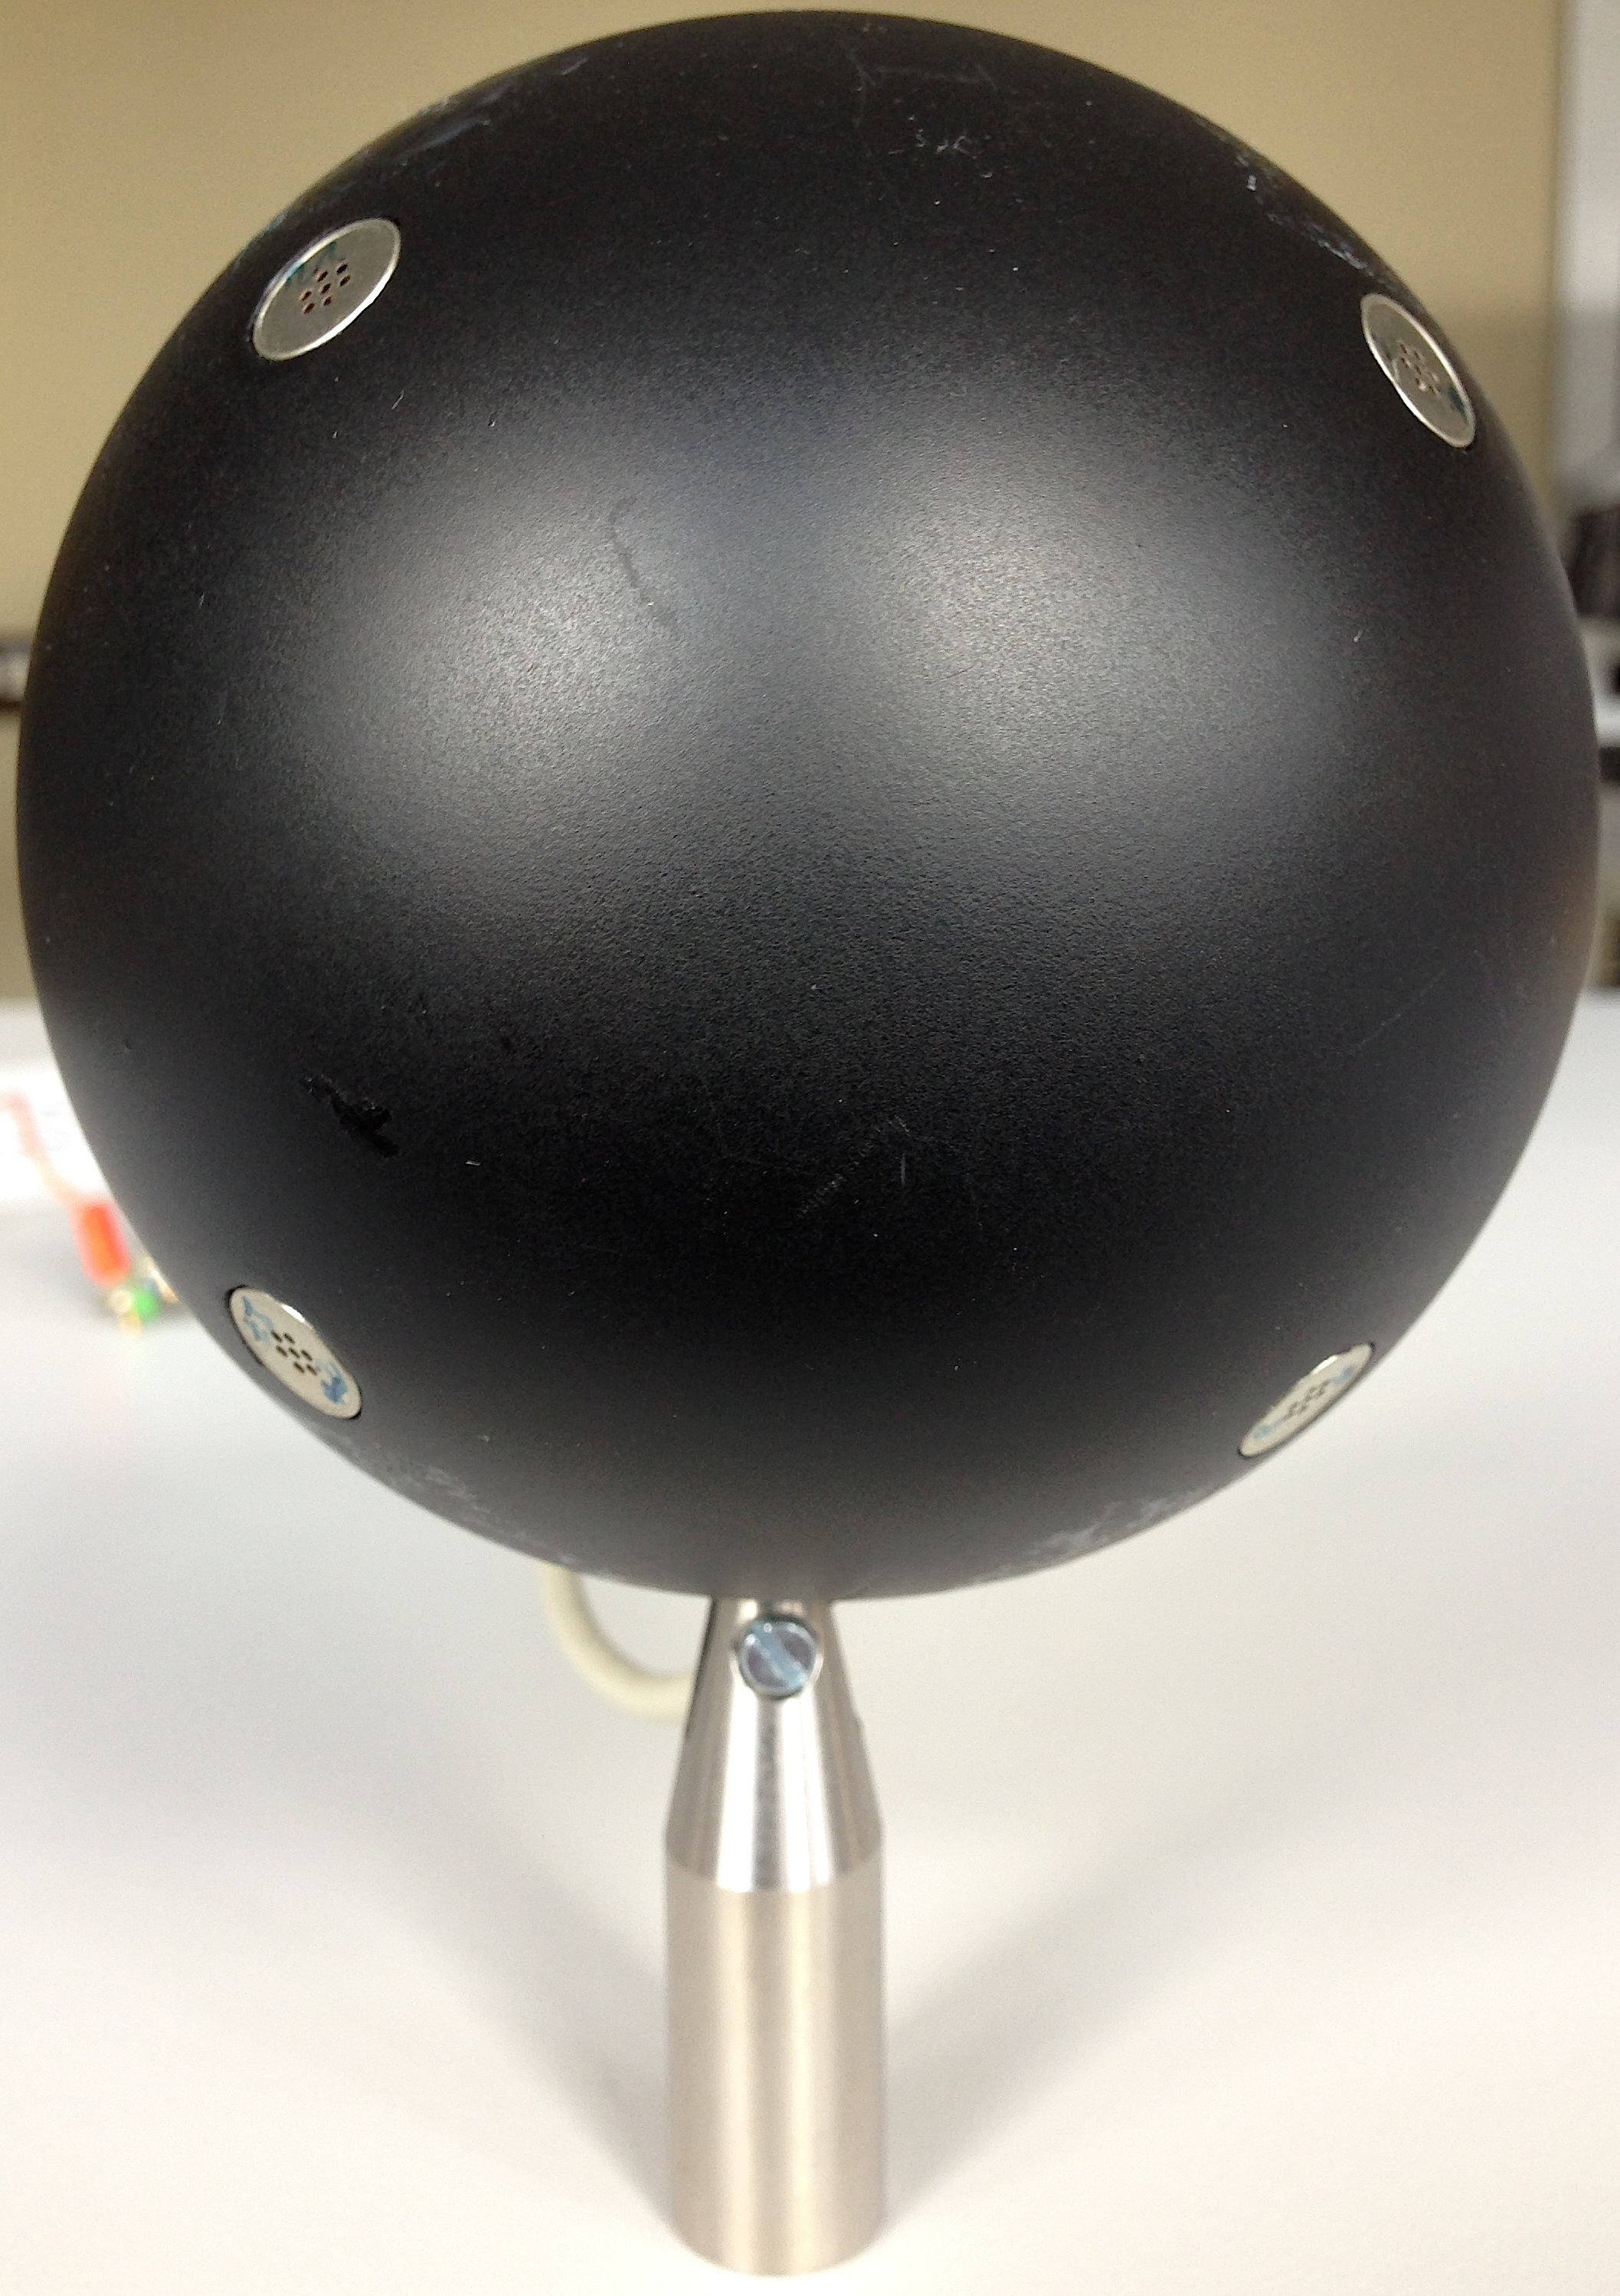
\includegraphics[width=\textwidth]{images/02_Konzeptionierung/Foto_MikrofonArray_Frontansicht}
                \caption{Frontansicht}
                \label{fig:Foto_MikrofonArray_Frontansicht}
        \end{subfigure}
        ~ %add desired spacing between images, e. g. ~, \quad, \qquad etc.
          %(or a blank line to force the subfigure onto a new line)
        \begin{subfigure}[b]{0.35\textwidth}
                \centering
                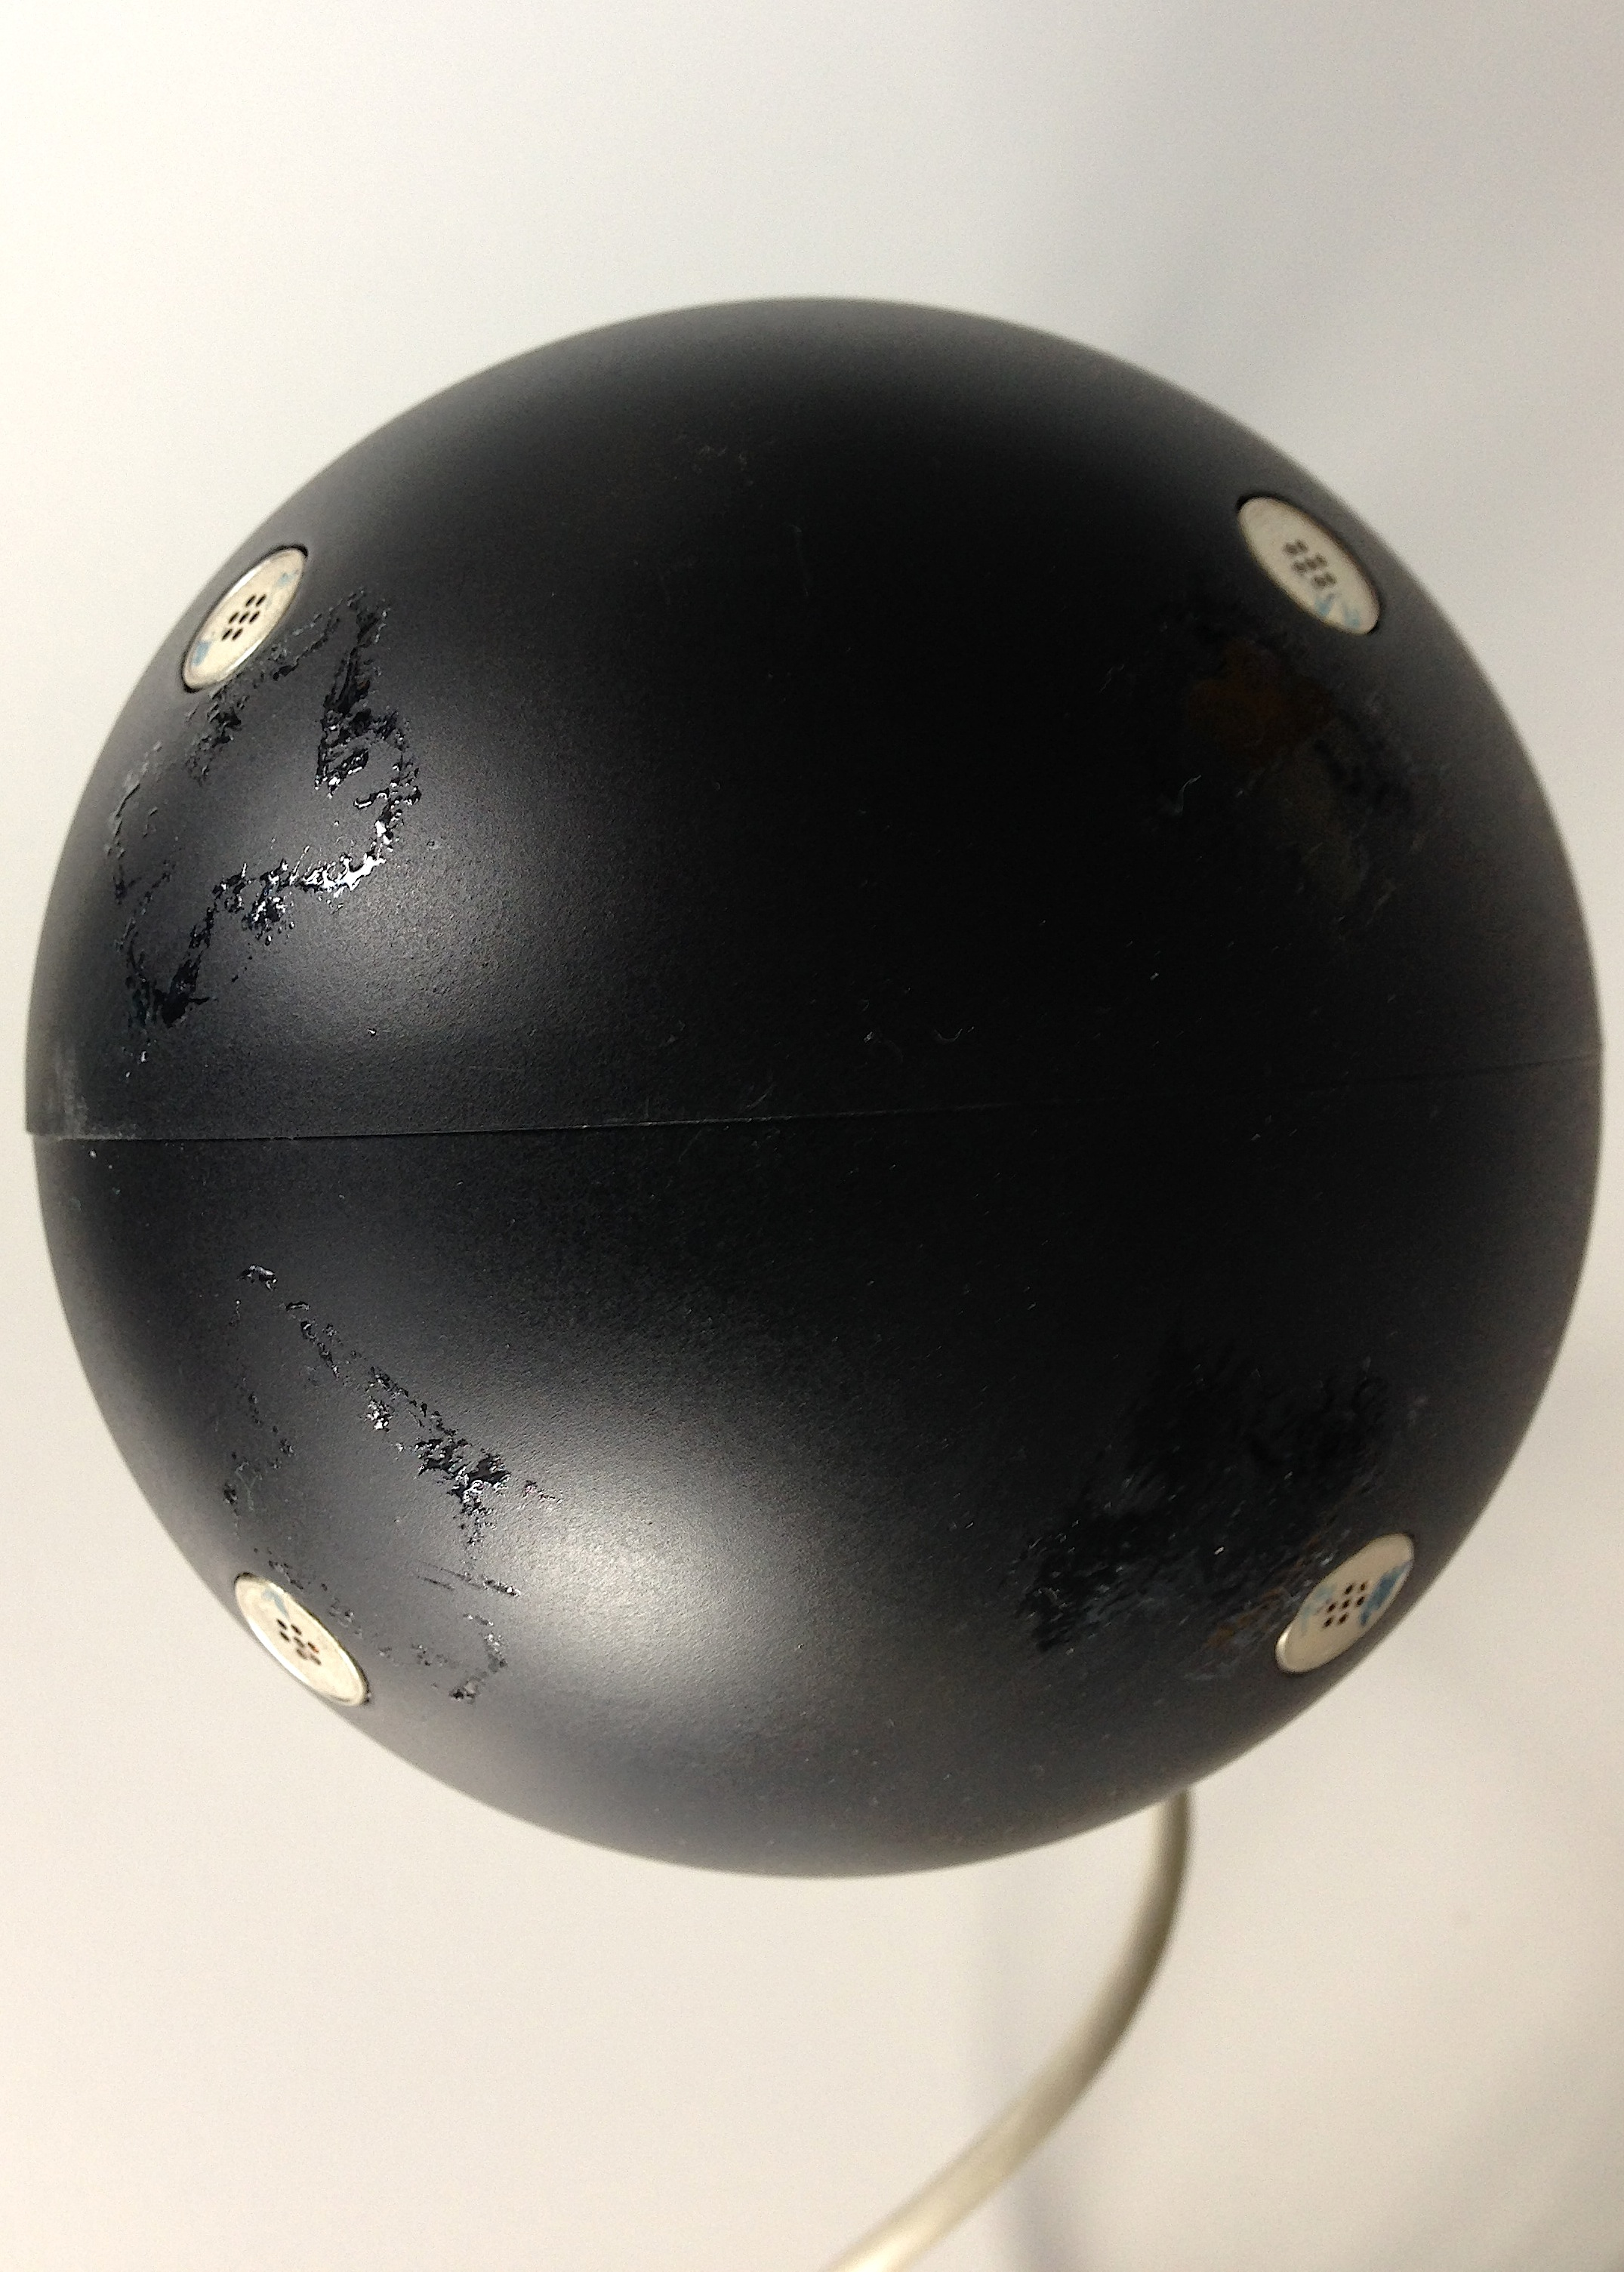
\includegraphics[width=\textwidth]{images/02_Konzeptionierung/Foto_MikrofonArray_Draufsicht}
                \caption{Draufsicht}
                \label{fig:Foto_MikrofonArray_Draufsicht}
        \end{subfigure}
        \caption{kugelförmiges Mikrofonarray}
        \label{fig:Foto_KugelfoermigesMikrofonarray}
\end{figure}
% ----------------------------------------- SUB-FIGURE -----------------------------------




\myFigure{real}                  % Figure tag (missing, real)
         {medium}                 % Size (small,medium,big)
         {h!}             % z.B. htbp
         {Sensoranordnung auf der Kugeloberfläche}                % Figure title
         {SensoranordnungKugeloberflaeche}                % Figure label 
         {02_Konzeptionierung/SensoranordnungKugeloberflaeche}     % Path to real figure








% ****************************************************************************************
\subsection{Untersuchung des kugelförmigen Mikrofonarrays}
\label{sec:UntersuchungKugelArrays}
% ****************************************************************************************
Zur Verifikation des angenommen Schallverhaltens an der schallharten Kugeloberfläche wird im folgenden eine Messung der Sensorlaufzeiten aus einer definierten Richtung durchgeführt und anschließend mit den theoretisch berechneten verglichen. \tab{KugelArray_Laufzeitmessung} zeigt einen tabellarischen Überblick der Messergebnisse. Der Fehler wird hier in Abtastwerten angegeben und bezieht sich auf eine Frequenz von $f_a=48kHz$. 

\begin{table}[h!]
     \center
     \begin{tabular}{cccc}
          \hline
          Sensorpaar & $\tau_{theo} [\mu s ]$ & $\tau_{gemessen} [\mu s ]$ & Fehler [Sample] \\
          \hline \hline
          $m_{13}$    &    272                  &  168                        & 5     \\
          $m_{14}$    &    184                & 168                       & 1  \\
          $m_{17}$    &    384                & 168                       & 11  \\
          $m_{24}$    &    288                  & 168                        & 6  \\
          $m_{28}$    &    384                  & 168                         & 11     \\
          \hline 
     \end{tabular}
  \caption{Laufzeitmessung an kugelförmigem Mikrofonarray bei den Winkeln $\phi=0°$, $\theta = 0°$.}
 \label{tab:KugelArray_Laufzeitmessung}
 \end{table}


Die bei dieser Messung auftretenden Fehler deuten darauf hin, dass sich die Schallwelle nicht wie erwartet geradlinig am Array vorbei bewegen, sondern mit großer Wahrscheinlichkeit an der Kugeloberfläche gebeugt wird. \abb{sim_wave_3000} zeigt eine Simulation (erstellt mit dem \matlab-Skript aus \cite{web_sim_wave}) die das Verhalten eines sinusförmigen Schall-Burst mit einer Frequenz von $f=3kHz$ an einer schallharten Kugel mit dem Radius $r=50mm$ untersucht. Es ist deutlich zu erkennen, dass die Schallwelle erheblich durch das Objekt beeinflusst wird. Eine theoretische Berechnung der Sensorlaufzeiten mit dem in \Sec{subsec:Sensormodell} beschriebenen Modell ist somit nicht möglich. Da das hier zu implementierende System nur mit diskreten Zeiten und somit mit diskreten Winkeln arbeitet können die ermittelten Fehler nicht toleriert werden. Ein Fehler von einem Abtastwert würde einen Fehler von einem Winkelschritt verursachen, wodurch eine zuverlässige Richtungsdetektion unmöglich wäre.


% ----------------------------------------- SUB-FIGURE -----------------------------------
\begin{figure}
        \centering
        \begin{subfigure}[b]{0.48\textwidth}
                \centering
                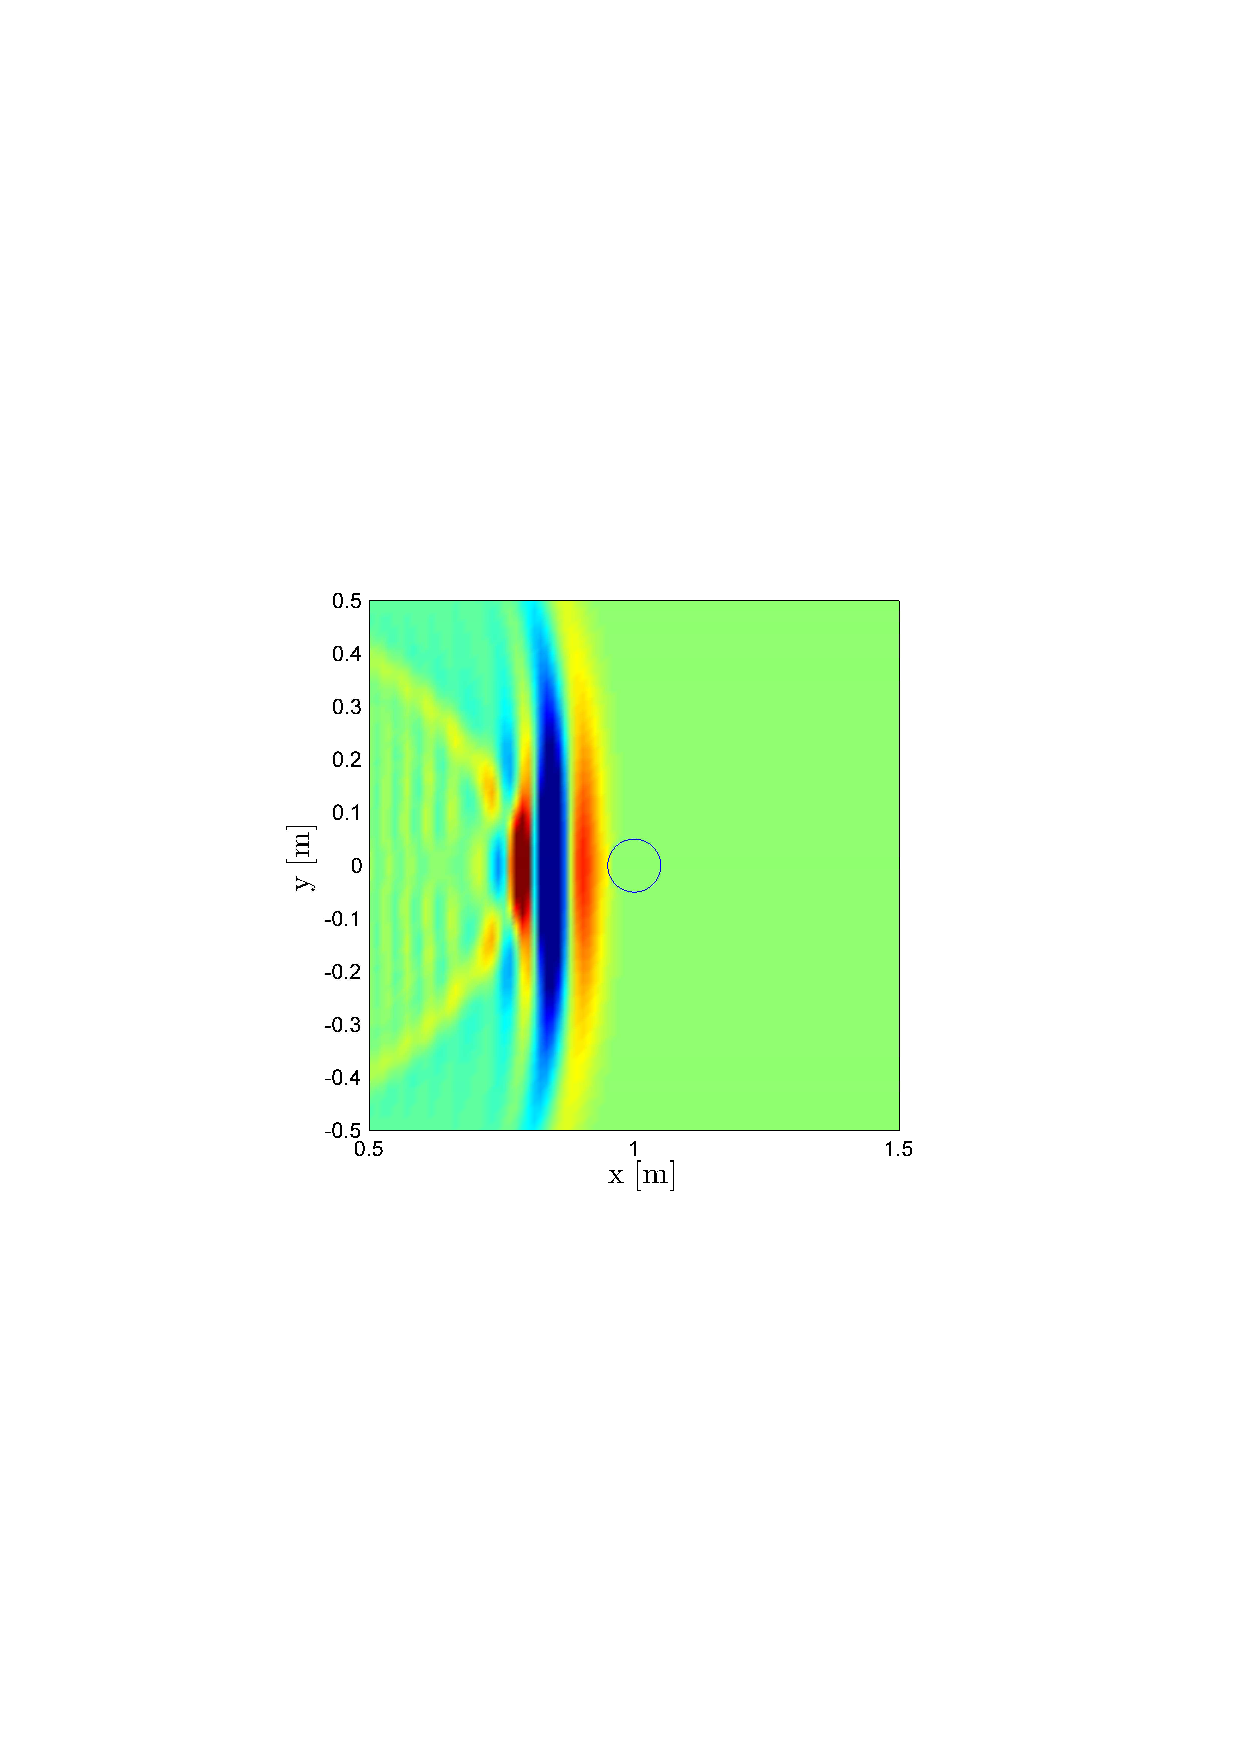
\includegraphics[width=\textwidth]{images/02_Konzeptionierung/sim_wave_3000_1}
                %\caption{Frontansicht}
                %\label{fig:sim_wave_3000_1}
        \end{subfigure}
        ~ %add desired spacing between images, e. g. ~, \quad, \qquad etc.
          %(or a blank line to force the subfigure onto a new line)
        \begin{subfigure}[b]{0.48\textwidth}
                \centering
                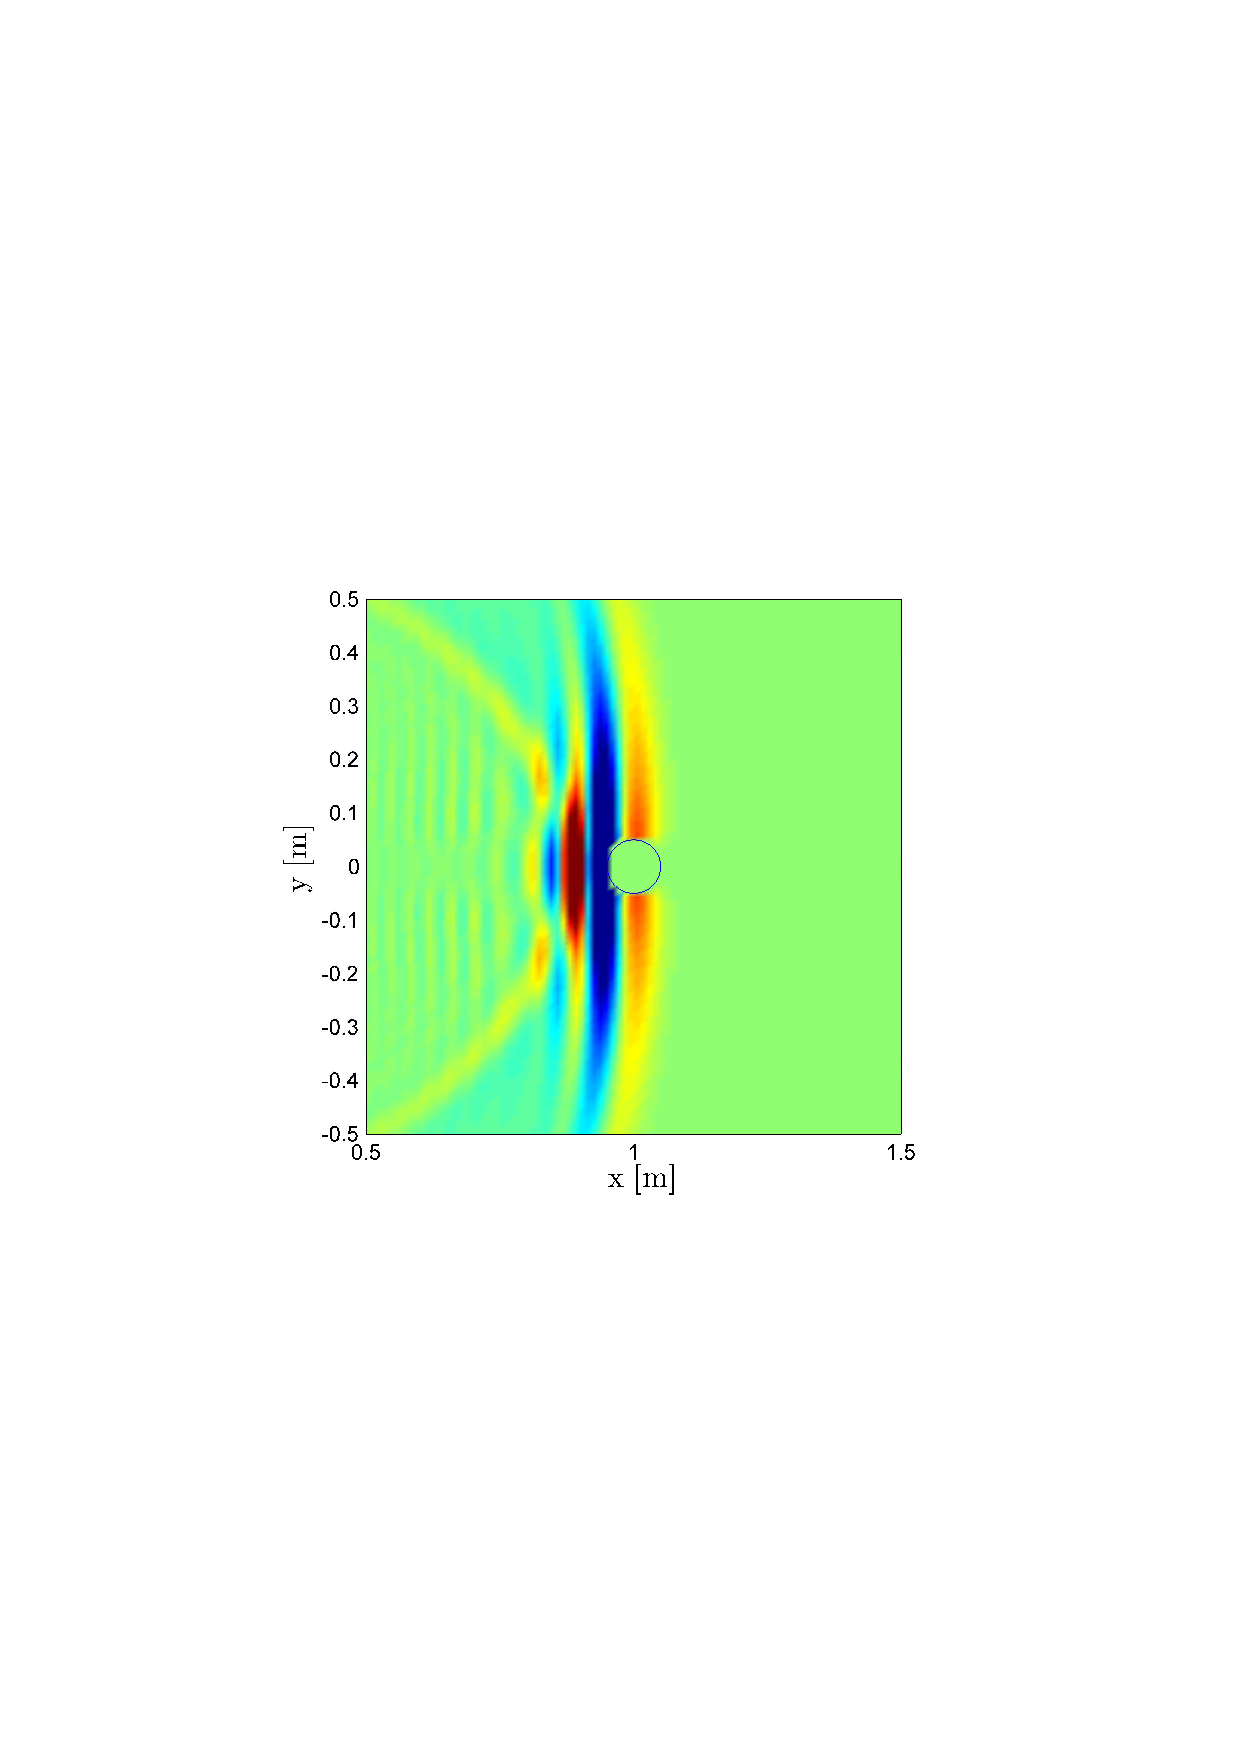
\includegraphics[width=\textwidth]{images/02_Konzeptionierung/sim_wave_3000_2}
                %\caption{Draufsicht}
                %\label{fig:sim_wave_3000_2}
        \end{subfigure}
        ~ %add desired spacing between images, e. g. ~, \quad, \qquad etc.
          %(or a blank line to force the subfigure onto a new line)
        \begin{subfigure}[b]{0.48\textwidth}
                \centering
                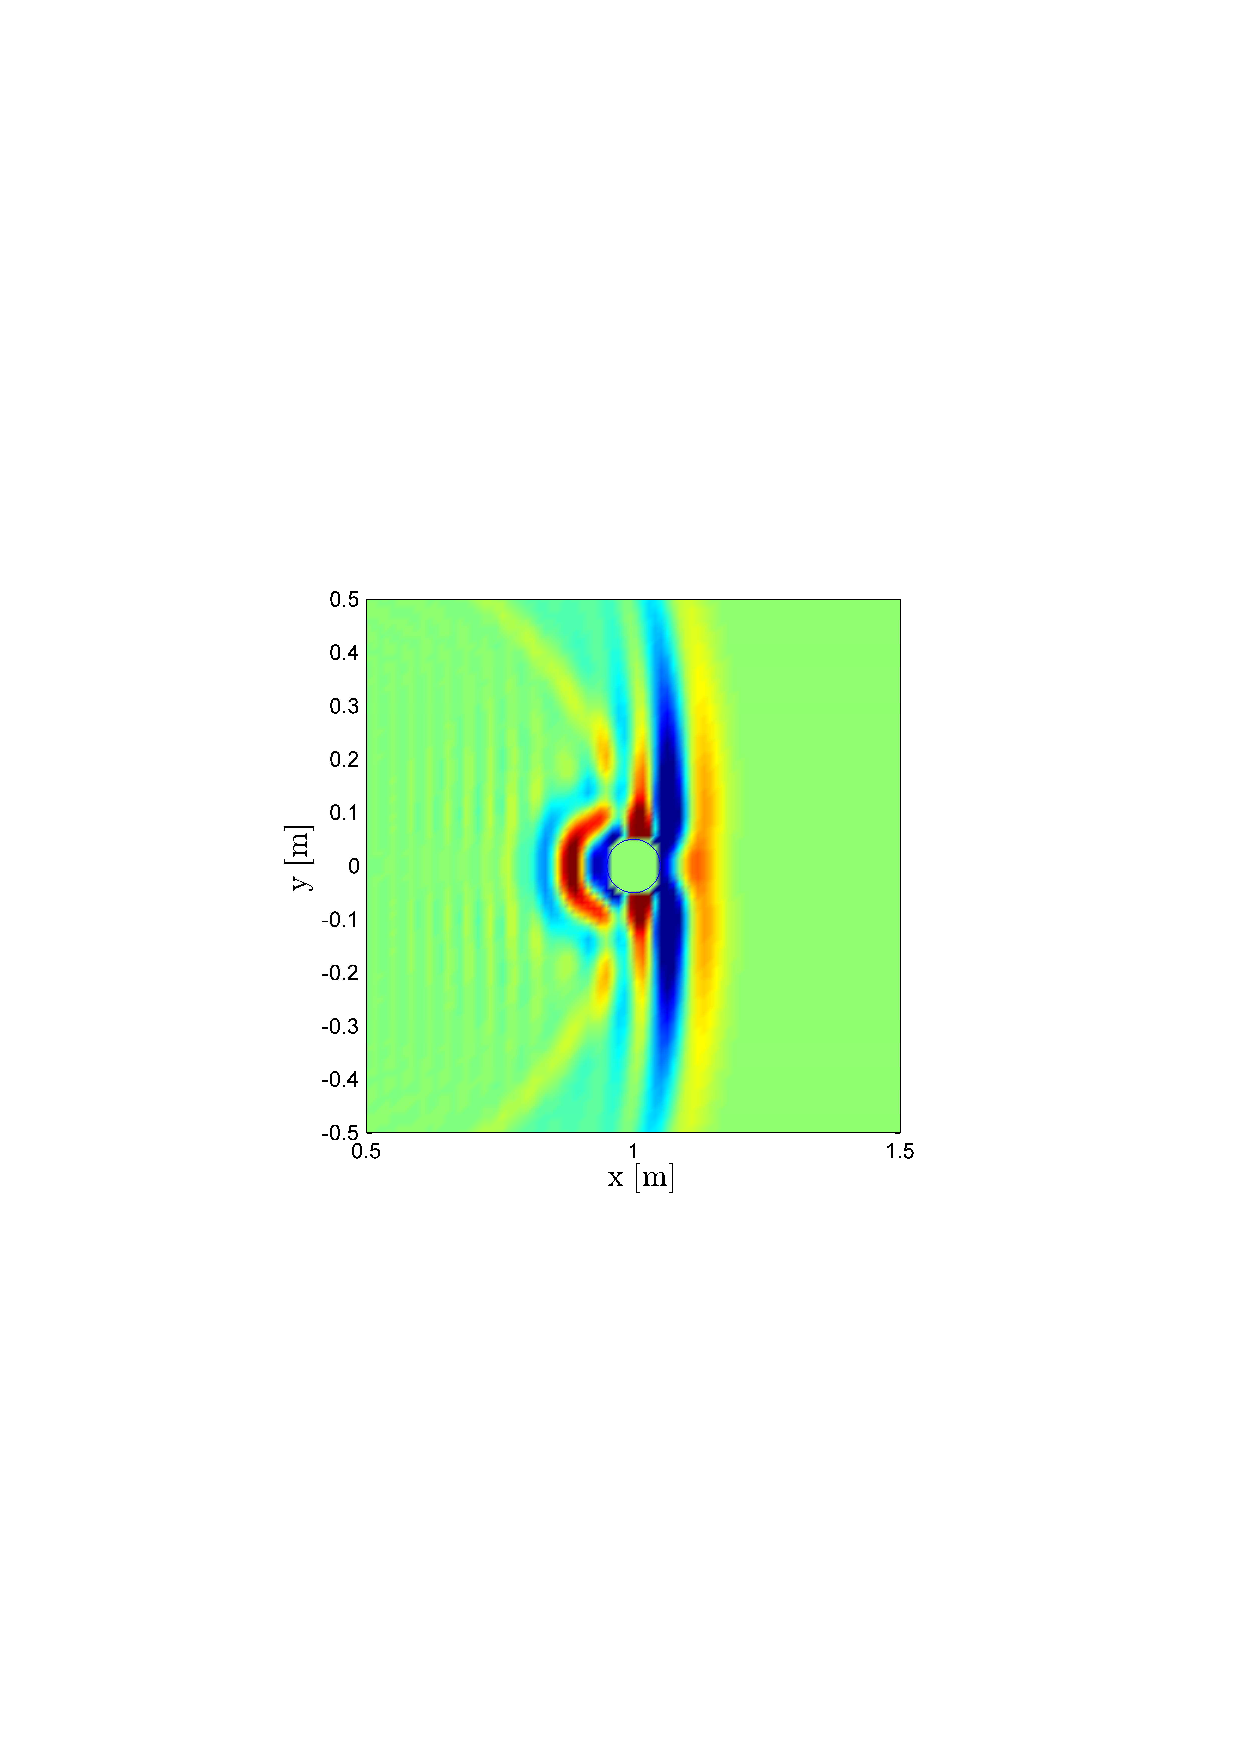
\includegraphics[width=\textwidth]{images/02_Konzeptionierung/sim_wave_3000_3}
                %\caption{Draufsicht}
                %\label{fig:sim_wave_3000_3}
        \end{subfigure}
        ~ %add desired spacing between images, e. g. ~, \quad, \qquad etc.
          %(or a blank line to force the subfigure onto a new line)
        \begin{subfigure}[b]{0.48\textwidth}
                \centering
                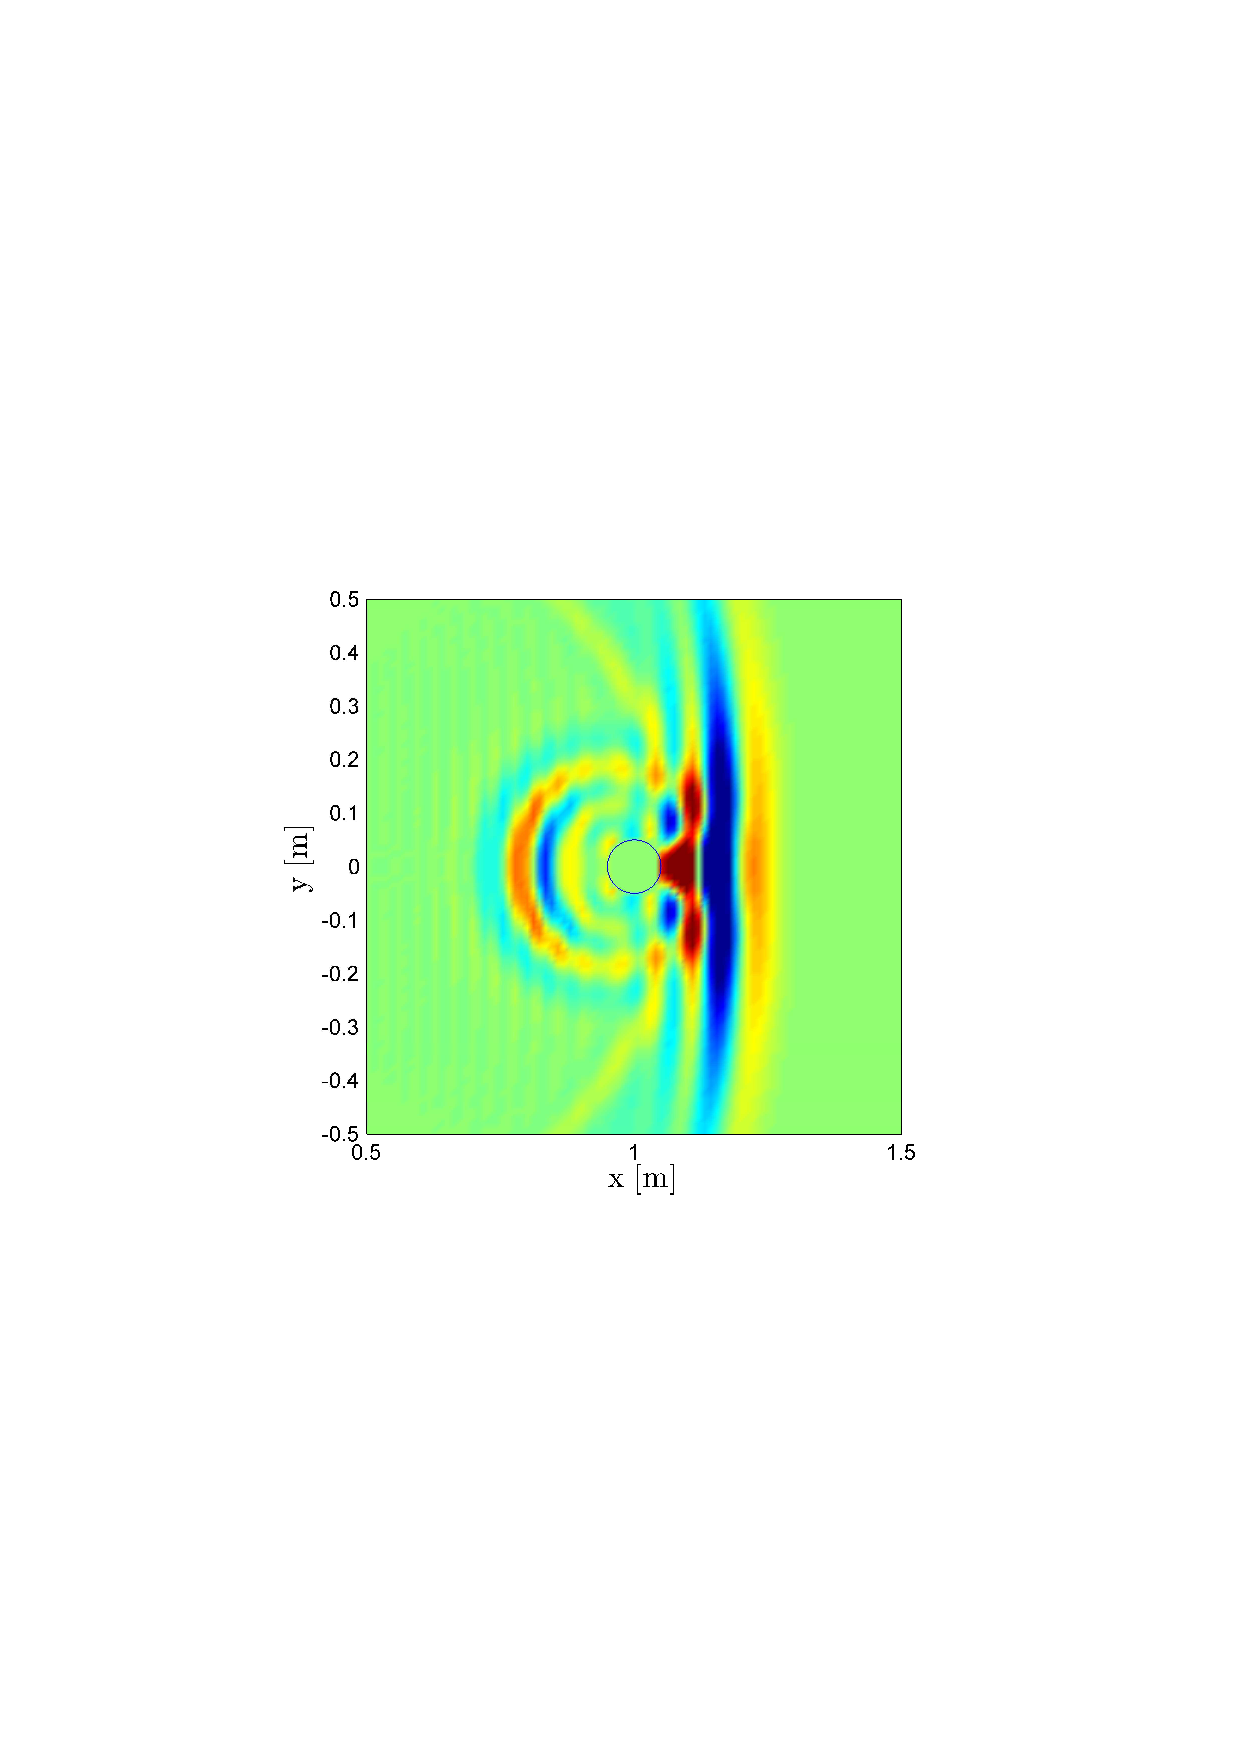
\includegraphics[width=\textwidth]{images/02_Konzeptionierung/sim_wave_3000_4}
                %\caption{Draufsicht}
                %\label{fig:sim_wave_3000_4}
        \end{subfigure}
        \caption{Schallverhalten an schallharter Kugel ($r=50mm$) mit einer Schallwelle der Wellenlänge $\lambda = 114mm$ und einer Frequenz von $f=3kHz$.}
        \label{fig:sim_wave_3000}
\end{figure}
% ----------------------------------------- SUB-FIGURE -----------------------------------






% ****************************************************************************************
\subsection{Mikrofonarray Neudesign/Konstruktion}
\label{subsec:MikrofonarrayNeudesign}
% ****************************************************************************************
Auf Basis der unter \Sec{sec:UntersuchungKugelArrays} gewonnen Erkenntnisse sowie der im \Sec{subsec:Sensormodell} erläuterten Zusammenhänge erfolgt in diesem Abschnitt eine Neukonstruktion des kugelförmigen Mikrofonarrays.

Um eine zuverlässige Aussage über die Schallausbreitung treffen zu können, muss der Körper des Mikrofonarray auf seine minimal nötigen Elemente reduziert werden. \abb{Prinzip_Konstruktion_NewArray} zeigt die prinzipielle Konstruktionsidee. Alle schallharten Bestandteile die einen unvorhersehbaren Einfluss auf die Schallausbreitung haben könnten, wurden entfernt, so dass der Körper nun lediglich aus dünnen Drähten besteht. Da sich die Mikrofonkapseln im Vergleich zur Kugel exakt an den selben Stellen befinden, kann dieses Array als Acht-Punkte-Approximation der Kugelgeometrie betrachtet werden.

Zur Prüfung des Schallverhaltens wurde der in \abb{Prototyp_Array} illustrierte Prototyp hergestellt. Die Drahtkonstruktion besteht dabei aus $1mm$ dicken Kupferdrähten, die an den Enden fest mit Lötzinn verbunden sind. Die Mikrofonkapseln wurden mit Hilfe von transparentem Kunststoff (Plexiglas) sowie Heißklebstoff in der oben beschriebenen Abstandsmetrik angeordnet. Die Kapseln selber wurden dabei im Hinblick auf eine spätere Mikrofonkonstruktion aus Pertinax\footnote{Phenolharz mit Papierfasern (sog. Hartpapier)}(inkl. einer dünnen Oberflächenschicht aus Kupfer) lediglich mit Klebeband fixiert.


\myFigure{real}                  % Figure tag (missing, real)
         {medium}                 % Size (small,medium,big)
         {h!}             % z.B. htbp
         {Prinzip der Mikrofonkonstruktion}                % Figure title
         {Prinzip_Konstruktion_NewArray}                % Figure label 
         {02_Konzeptionierung/Prinzip_Konstruktion_NewArray}     % Path to real figure



\myFigure{real}                  % Figure tag (missing, real)
         {medium}                 % Size (small,medium,big)
         {h!}             % z.B. htbp
         {Prototyp des würfelförmigen Mikrofonarrays}                % Figure title
         {Prototyp_Array}                % Figure label 
         {02_Konzeptionierung/Prototyp_Array}     % Path to real figure



% ****************************************************************************************
\subsubsection{Laufzeitmessung am Prototyp}
% ****************************************************************************************
\tab{Prototyp_NewArray_Laufzeitmessung} zeigt die Ergebnisse von zwei Laufzeitmessungen aus unterschiedlichen Schalleinfallsrichtungen. Gemessen wurden immer die Laufzeitdifferenzen zum Referenzmikrofon $M_1$. Zur Verifikation der Geometrie wurde das Array mit einem durch einen Lautsprecher abgestrahlten Rechteckimpuls angeregt. Die dazu benötigten theoretischen Laufzeitdifferenzen wurden mit der in \Eq{DOA_winkel} eingeführten Mikrofonfunktion $f_n(\phi, \theta)$ errechnet. Die Differenz zwischen theoretischem und gemessenem Wert wird als Anzahl von Abtastwerten mit einer Frequenz von $f_a = 48kHz$ angegeben. Die Messergebnisse weichen nur leicht von den theoretisch berechneten ab, so dass sich die Arraykonstruktion aus dünnen Drähten als geeignet erweist.

Da die Konstruktion, bedingt durch die dünnen Kupferdrähte, mechanisch sehr instabil ist und die Mikrofonkapseln im Vergleich zur Kugel nicht exakt gleich angeordnet sind, wird im Folgenden eine Neukonstruktion des Array vorgestellt.


\begin{table}[]
     \center
     \begin{tabular}{cccc}
          \hline
          Sensorpaar & $\tau_{theo} [\mu s ]$ & $\tau_{gemessen} [\mu s ]$ & Fehler [Sample] \\
          \hline \hline
          $\phi = 0°, \theta = 0°$ \\
          \hline
          $m_{12}$    &    0                  &  0                        & 0        \\
          $m_{13}$    &    168                & 165                       & 0,14        \\
          $m_{14}$    &    168                & 162                       & 0,28        \\
          $m_{15}$    &    0                  & 12                        & 0,57       \\
          $m_{16}$    &    0                  & 0                         & 0        \\
          $m_{17}$    &    168                & 155                       & 0,62    \\
          $m_{18}$    &    168                & 150                       & 0,84    \\
          \hline
            %          &                       &            Mittelwert     & 0,19    \\
          \hline
          $\phi = 45°, \theta = 45°$ \\
          \hline
          $m_{12}$    &   -84                 &  -90                      & 0,28        \\
          $m_{13}$    &    0                  & 0                         & 0        \\
          $m_{14}$    &    84                 & 84                        & 0        \\
          $m_{15}$    &    119                & 112                       & 0,33       \\
          $m_{16}$    &    34                 & 50                        & -0,76        \\
          $m_{17}$    &    119                & 130                       & -0,52    \\
          $m_{18}$    &    203                & 190                       & 0,62    \\
          %\hline
          %            &                       &            Mittelwert     & 0    \\
          \hline 
     \end{tabular}
  \caption{Laufzeitmessung aus zwei unterschiedlichen Schalleinfallsrichtungen}
 \label{tab:Prototyp_NewArray_Laufzeitmessung}
 \end{table}
 

%\todo[inline]{Hier eine Grafik mit Matlab ploten und für jede Richting (also ein paar Winkelpaare) mit der Formel aus von Benesty einfügen um die Genauigkeit darzustelln K=Anzahl der gemessenen Mikrofonpaare $f_{Stabw}(\phi, \theta) = \sqrt{\frac{1}{K-1} \sum_{i=1}^{K} \left[ f_{theory}(\phi, \theta) - f_i(\phi, \theta) \right]^2}$}



% Bilder zur Laufzeitmessung
% ----------------------------------------- SUB-FIGURE -----------------------------------
%\begin{figure}
%        \centering
%        \begin{subfigure}[b]{0.48\textwidth}
%                \centering
%                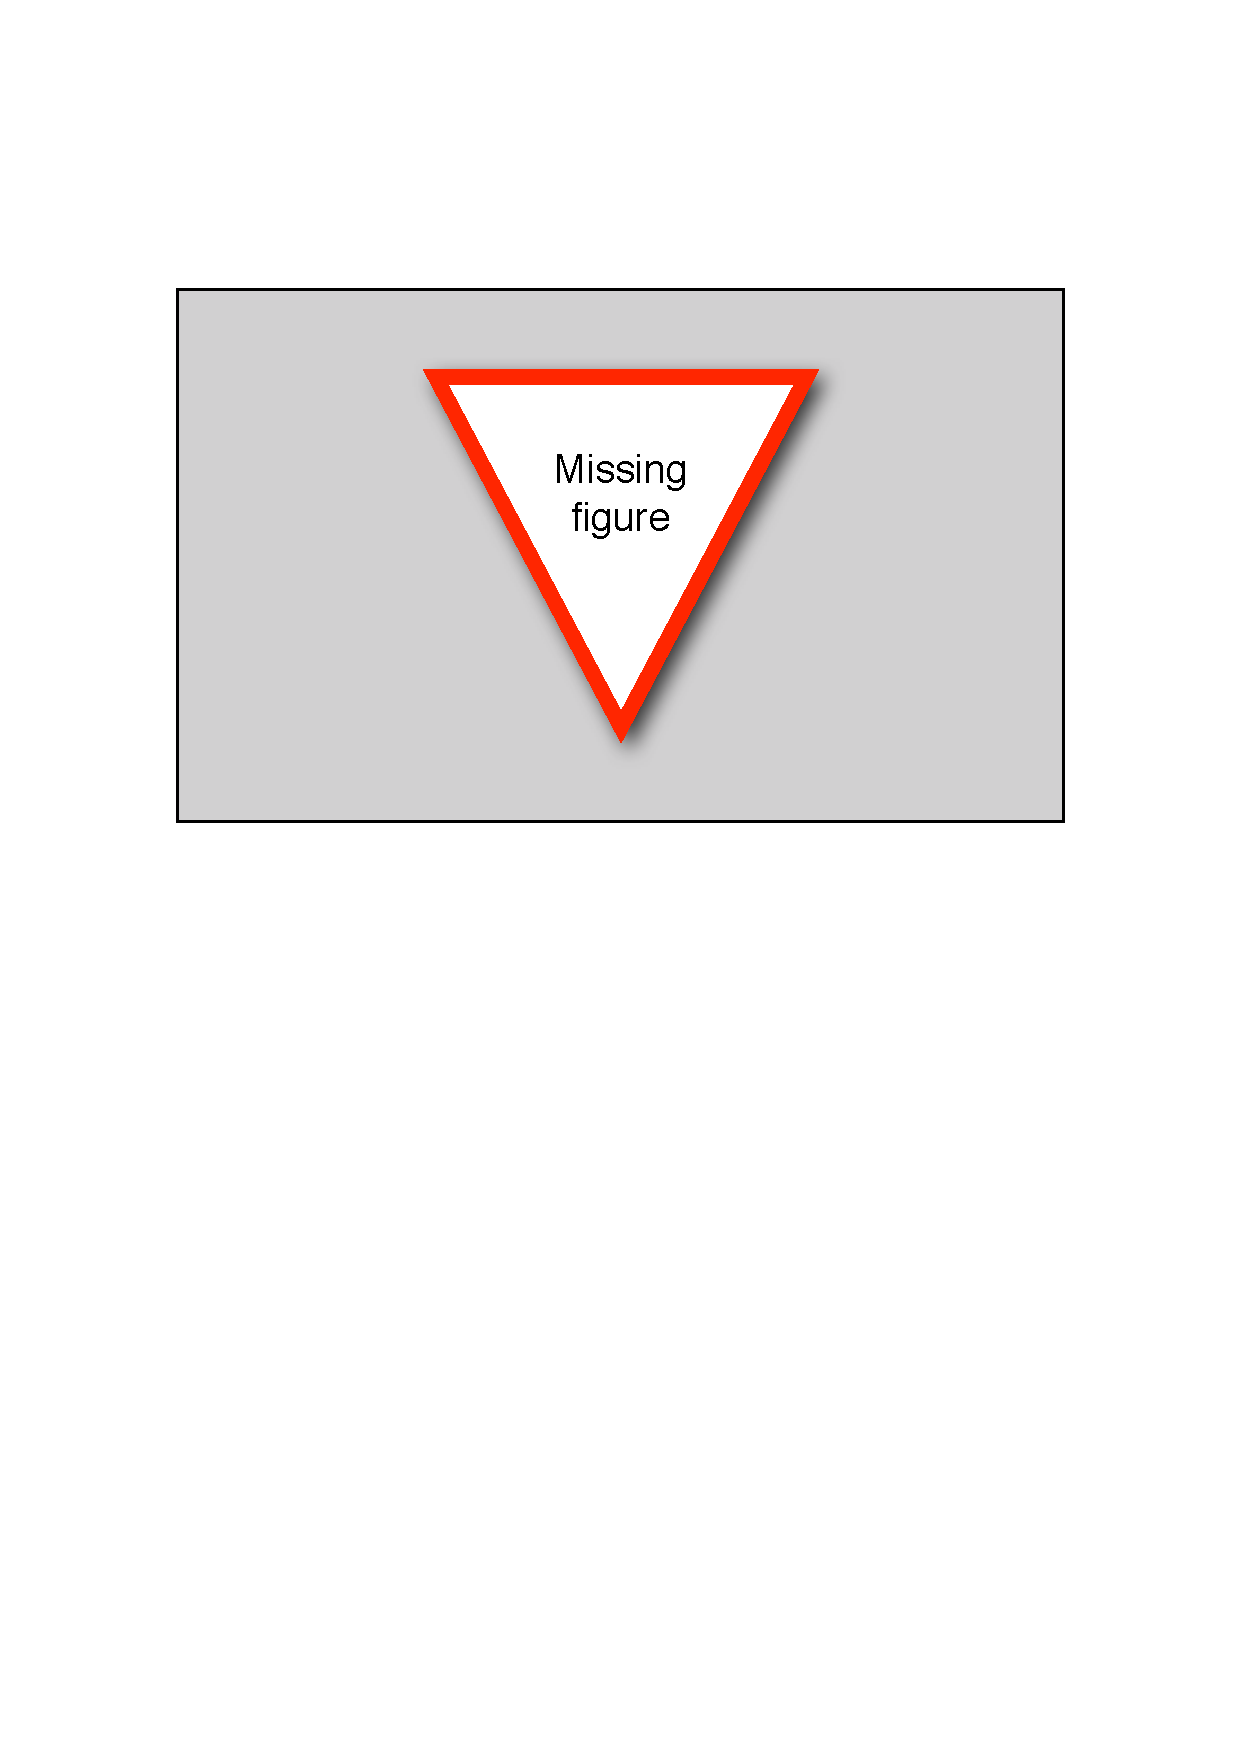
\includegraphics[width=\textwidth]{images/MissingFigure}
%                \caption{$\phi=0°, \theta=0°$}
%                \label{fig:Richtung1}
%        \end{subfigure}
%        ~ %add desired spacing between images, e. g. ~, \quad, \qquad etc.
%          %(or a blank line to force the subfigure onto a new line)
%        \begin{subfigure}[b]{0.48\textwidth}
%                \centering
%                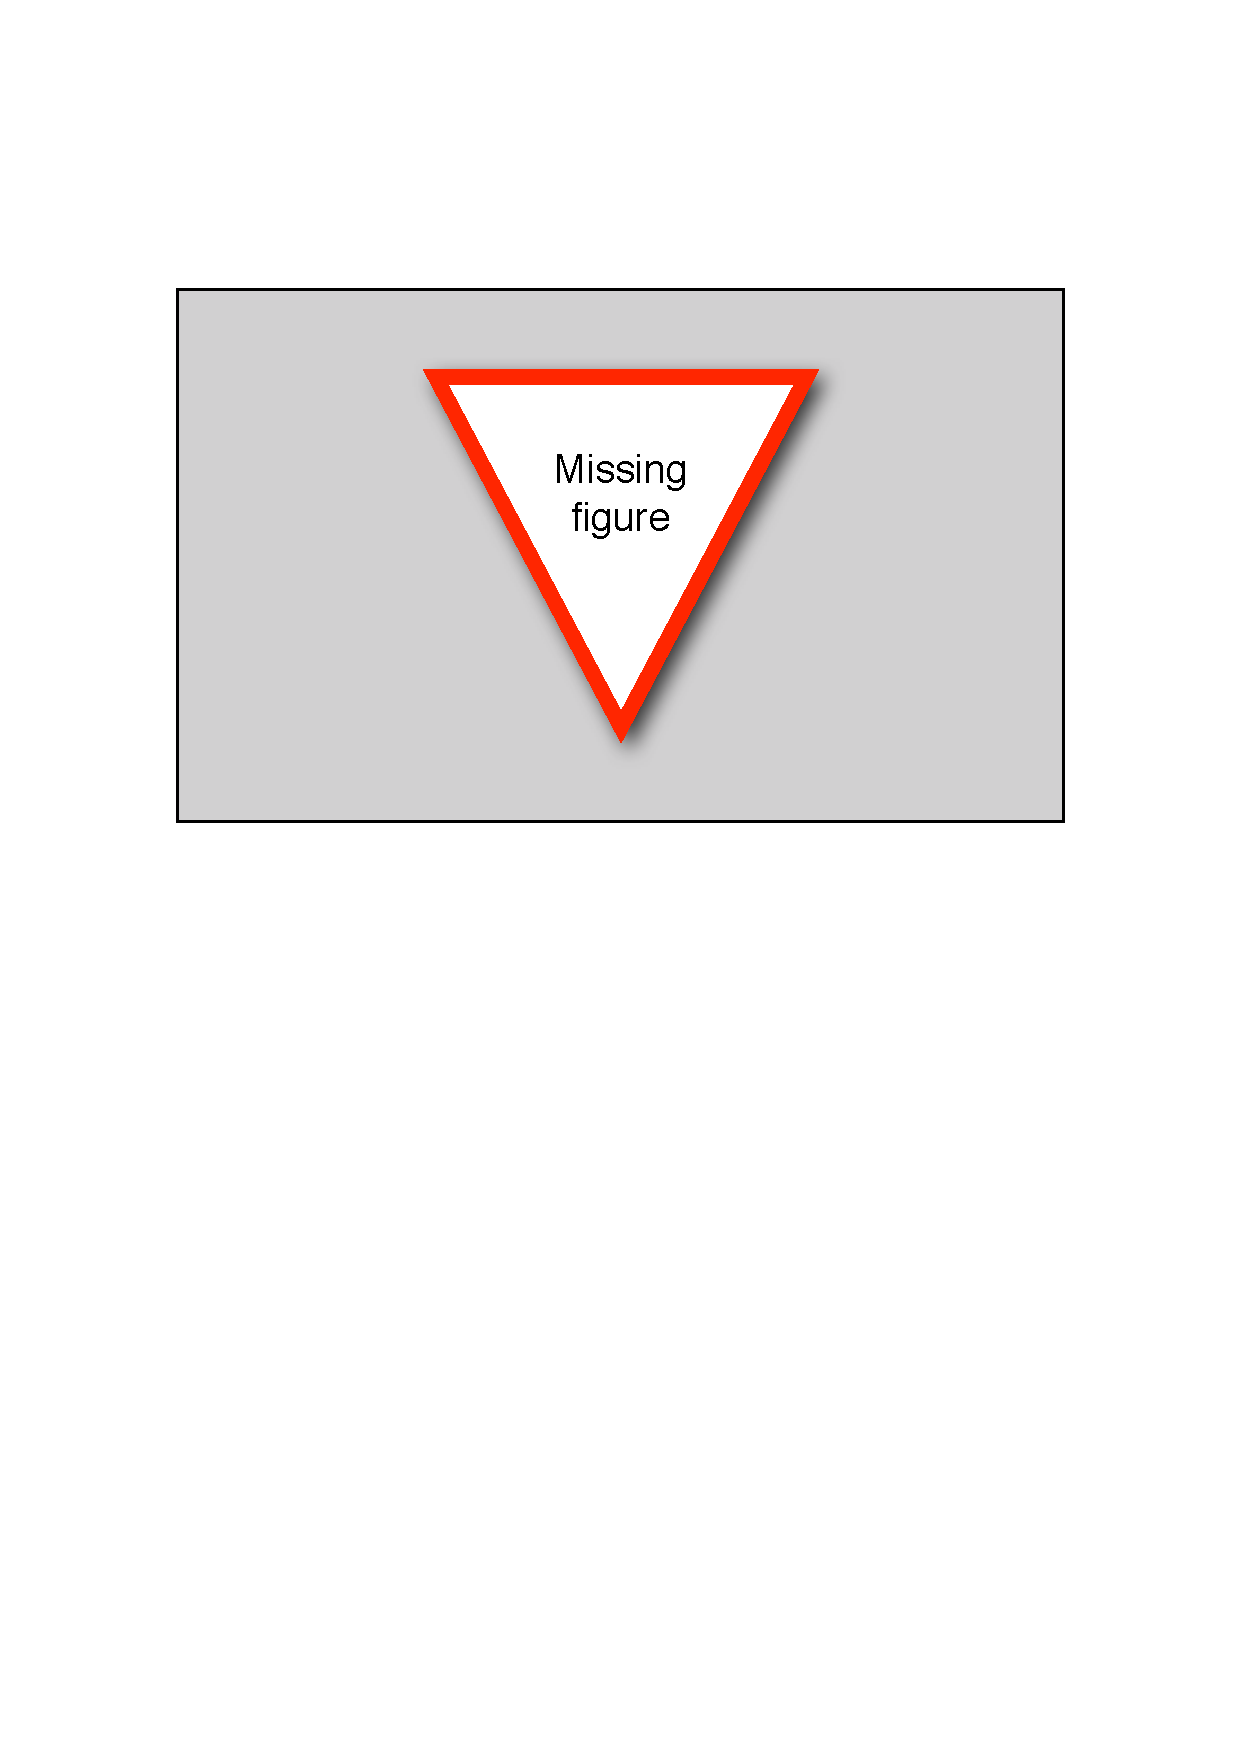
\includegraphics[width=\textwidth]{images/MissingFigure}
%                \caption{$\phi=0°, \theta=45°$}
%                \label{fig:Richtung2}
%        \end{subfigure}
%        ~
%        \begin{subfigure}[b]{0.48\textwidth}
%                \centering
%                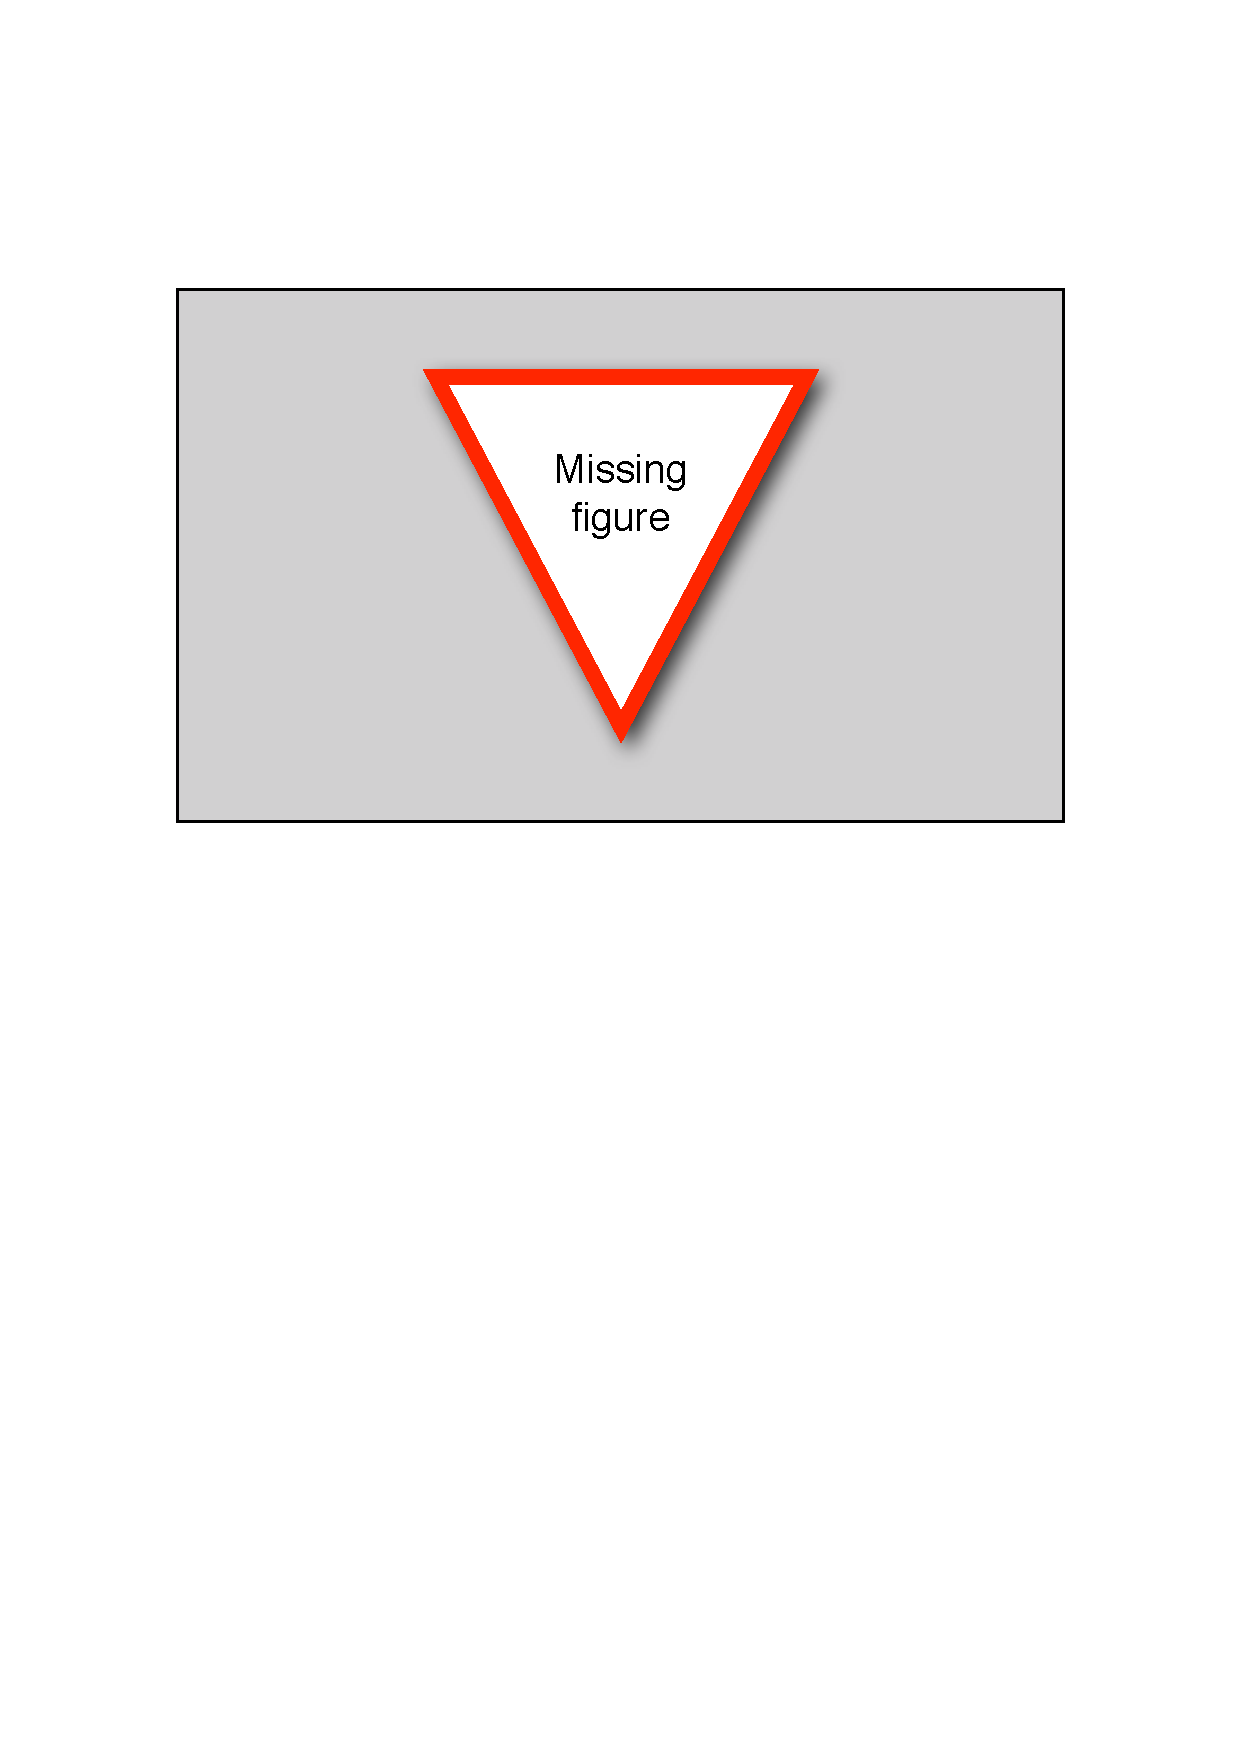
\includegraphics[width=\textwidth]{images/MissingFigure}
%                \caption{$\phi=45°, \theta=0°$}
%                \label{fig:Richtung3}
%        \end{subfigure}
%        ~
%        \begin{subfigure}[b]{0.48\textwidth}
%                \centering
%                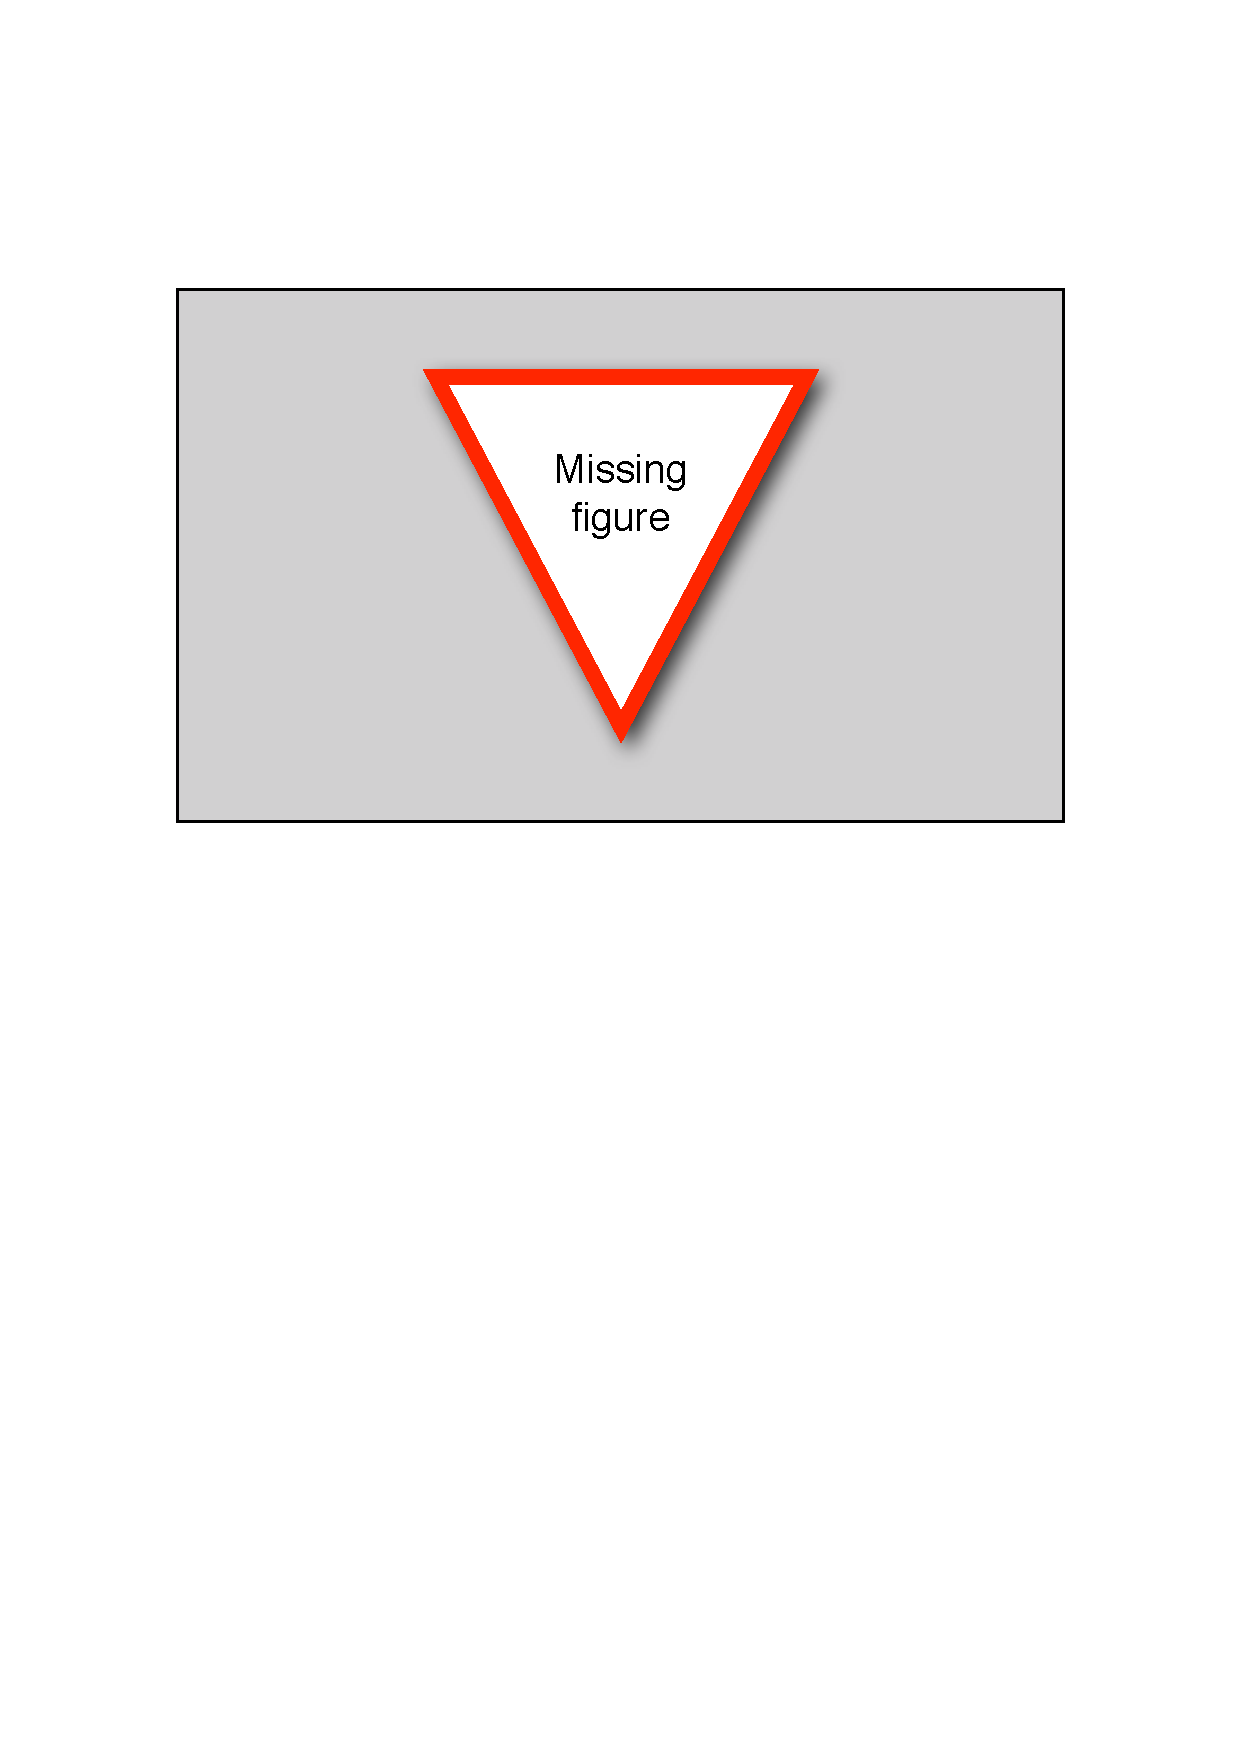
\includegraphics[width=\textwidth]{images/MissingFigure}
%                \caption{$\phi=45°, \theta=45°$}
%                \label{fig:Richtung4}
%        \end{subfigure}
%        \stepcounter{missingFigureCount}
%        \caption{\textbf{\textcolor{red}{Missing Figure \themissingFigureCount}} - Laufzeitmessung am Array-Prototyp}
%        \label{fig:Prototyp_NewArray_Laufzeitmessung}
%\end{figure}
% ----------------------------------------- SUB-FIGURE -----------------------------------


















% ****************************************************************************************
\subsubsection{Äquidistante Arraykonstruktion}
% ****************************************************************************************
Auf Basis der Array-Prototyp Idee wird in diesem Abschnitt ein Array entwickelt, das über eine ausreichend hohe Genauigkeit sowie mechanische Festigkeit verfügt.

Zur Bestimmung der minimal nötigen Herstellungsgenauigkeit wird die Eigenschaft des hier vorliegenden diskreten Systems genutzt. Auf Grund der Zeitdiskretisierung können nur Laufzeitdifferenzen gemessen werden, die ein Vielfaches der Abtastperiode $T_a$ betragen. Die Strecke $d_{T_a}$, die vom Schall innerhalb einer Abtastperiode zurückgelegt wird, ergibt sich durch

\begin{equation}
    d_{T_a} = c \cdot T_a = \frac{c}{f_a}
\end{equation}

\tab{Toleranz_Abtastfrequenz} zeigt unterschiedliche Toleranzbereiche bei den im Audiobereich gängigen Abtastraten. Um einen Messfehler der Laufzeitdifferenz zu vermeiden, muss der entsprechende Toleranzbereich eingehalten werden.


\begin{table}[h]
     \center
     \begin{tabular}{ccc}
     \hline
          Abtastfrequenz [kHz] & $d_{T_a}$ [mm] & Toleranz [mm] \\
           \hline \hline
          8                    & 42,8           & $\pm 21,4$\\
          16                   & 21,4           & $\pm 10,7$\\
          24                   & 14,3           & $\pm 7,1$\\
          48                   & 7,1            & $\pm 3,5$\\
          96                   & 3,5            & $\pm 1,8$\\
         \hline
     \end{tabular}
  \caption{Toleranzbereich bei unterschiedlichen Abtastfrequenzen}
 \label{tab:Toleranz_Abtastfrequenz}
 \end{table}


Als grundsätzliche Konstruktionsidee wird hier ein Steckmechanismus eingesetzt. Die Einzelteile können so aus einem flachen Werkstoff (\zB einer Blechtafel oder Pertinaxplatten) ausgeschnitten werden. Fertigungsprozesse solcher Art sind aufwandsarm da die Einzelteile mit einem CNC\footnote{Computerized Numerical Control}-Laser oder einer CNC-Wasserschneidemaschine aus großen Werkstofftafeln ausgearbeitet werden können. Auf Grund der hohen Schneidegeschwindigkeit moderner Werkzeugmaschinen und der geringen Einricht -und Spannzeit kann solch eine Konstruktion bereits in geringer Stückzahl kostengünstig hergestellt werden.

Zur Befestigung der einzelnen Teile miteinander werden, wie in \abb{3D_Konstruktion_Steckmechanismus} dargestellt, entsprechende Ausschnitte eingearbeitet an denen diese dann zusammengesteckt werden. Um eine ausreichend hohe Festigkeit der Steckverbindung zu gewährleisten, werden diese Ausschnitte entsprechend einer Übergangspassung angefertigt. \abb{3D_Konstruktion_Geundkoerper} zeigt die beiden X-förmigen Grundelemente der Konstruktion. Diese bilden nach dem Zusammenstecken die vier durch das Zentrum laufenden Streben der in \abb{Prinzip_Konstruktion_NewArray} gezeigten Prinzipskizze.

Zur Befestigung der empfindlichen Mikrofonkapseln wird ebenfalls ein Steckmechanismus entworfen. Wie in \abb{3D_Konstruktion_Mikrofonhalterung} illustriert, besteht die Halterung aus einem kleinen Stück Pertinax mit einem halboffenen kreisrunden Ausschnitt. Der Durchmesser dieses Halbkreises entspricht exakt dem der Mikrofonkapsel von $9,7mm$ wobei an den beiden Ecken der Öffnung zwei nach innen ragenden Rundungen angebracht sind. Diese werden beim Einstecken nach außen gebogen und sorgen für eine ausreichend hohe Klemmkraft zum Fixieren der Kapsel. Durch diesen Mechanismus lassen sich die Mikrofone nach dem Einbau feinjustieren und können darüber hinaus leicht aus dem Array entfernt werden.




\myFigure{real}                  % Figure tag (missing, real)
         {small}                 % Size (small,medium,big)
         {h!}             % z.B. htbp
         {Prinzip des Steckmechanismus}                % Figure title
         {3D_Konstruktion_Steckmechanismus}                % Figure label 
         {02_Konzeptionierung/3D_Konstruktion_Steckmechanismus.pdf}     % Path to real figure




\myFigure{real}                  % Figure tag (missing, real)
         {small}                 % Size (small,medium,big)
         {h!}             % z.B. htbp
         {Grundkomponenten des Mikrofonarrays}                % Figure title
         {3D_Konstruktion_Geundkoerper}                % Figure label 
         {02_Konzeptionierung/3D_Konstruktion_Grundkoerper.pdf}     % Path to real figure


\myFigure{real}                  % Figure tag (missing, real)
         {medium}                 % Size (small,medium,big)
         {h!}             % z.B. htbp
         {Haltemechanismus der Mikrofonkapseln}                % Figure title
         {3D_Konstruktion_Mikrofonhalterung}                % Figure label 
         {02_Konzeptionierung/3D_Konstruktion_Mikrofonhalterung.pdf}     % Path to real figure




Um die Mikrofonkapseln im Vergleich zur Kugelgeometrie exakt gleich auszurichten, wird die gesamte Arraygeometrie, wie in \abb{3D_Konstruktion_Array_Verdrehung} dargestellt, um einen Winkel von $16°$ gedreht. Die Mikrofone sind so für den Schall von allen Seiten ohne direktes Hindernis erreichbar. Der Abstand zwischen zwei gegenüberliegenden Kapseln beträgt wie oben genannt $100mm$, so dass sich die Kapseloberseite, wie in \abb{3D_Konstruktion_Array_mit_Kugel} gezeigt, genau auf der Kugeloberfläche befindet. Die in blau eingezeichneten Linien stellen dabei die gedachten Würfelkanten dar und sind somit in der realen Konstruktion nicht vorhanden.


\myFigure{real}                  % Figure tag (missing, real)
         {small}                 % Size (small,medium,big)
         {h!}             % z.B. htbp
         {Drehung der Arraygeometrie zur exakten Positionierung der Mikrofonkapseln}                % Figure title
         {3D_Konstruktion_Array_Verdrehung}                % Figure label 
         {02_Konzeptionierung/3D_Konstruktion_Array_Verdrehung.pdf}     % Path to real figure


\myFigure{real}                  % Figure tag (missing, real)
         {small}                 % Size (small,medium,big)
         {h!}             % z.B. htbp
         {Vergleich zwischen Kugel- und Würfelgeometrie}                % Figure title
         {3D_Konstruktion_Array_mit_Kugel}                % Figure label 
         {02_Konzeptionierung/3D_Konstruktion_Array_mit_Kugel}     % Path to real figure


Die doppel-x-förmige Konstruktion bildet somit die Kugeloberfläche genau an den acht Mikrofonpositionen ab. Des weiteren ist der Grundkörper, wie in \abb{3D_Konstruktion_Teleskop_Arm} dargestellt, mittels verschiebbaren Verlängerungsstreben versehen. Mit diesen ist es möglich, den Mikrofonabstand stufenlos bis auf $147mm$ zu vergrößern.




\myFigure{real}                  % Figure tag (missing, real)
         {small}                 % Size (small,medium,big)
         {h!}             % z.B. htbp
         {Variabel verstellbare Mikrofonabstände}                % Figure title
         {3D_Konstruktion_Teleskop_Arm}                % Figure label 
         {02_Konzeptionierung/3D_Konstruktion_Teleskop_Arm}     % Path to real figure



Zur Herstellung des Prototypen wird die in \abb{3D_Konstruktion_Fertigung} dargestellte CNC-Fräsmaschine eingesetzt. Diese verfügt über eine Toleranz von $\pm 0,1 mm$ und liegt damit weit unter der minimal nötigen Toleranz in \tab{Toleranz_Abtastfrequenz}. Die Einzelteilkonstruktionen müssen hierfür in das DXF\footnote{Drawing Interchange File Format}-Dateiformat konvertiert werden, wodurch sie ohne weitere Maschinenprogrammierung direkt zur Fertigung verwendet werden könnten. Zu beachten ist, dass die Software der Maschine keine Korrektur der Fräserabmaße vornimt. Jedes Einzelteil muss diesbezüglich erneut bearbeitet werden, so dass alle Außenkonturen um den Fräserradius vergrößert und alle Innenkonturen um den Fräserradius verkleinert werden. \abb{Vergleich_array_gefertigt} zeigt das zusammengesetzte sowie verdrahtete Mikrofonarray.


\myFigure{real}                  % Figure tag (missing, real)
         {big}                 % Size (small,medium,big)
         {h!}             % z.B. htbp
         {Fertigung der Einzelteile unter Verwendung einer CNC-Fräsmaschine}                % Figure title
         {3D_Konstruktion_Fertigung}                % Figure label 
         {02_Konzeptionierung/3D_Konstruktion_Fertigung}     % Path to real figure


 % ----------------------------------------- SUB-FIGURE -----------------------------------
\begin{figure}
        \centering
        \begin{subfigure}[b]{0.4\textwidth}
                \centering
                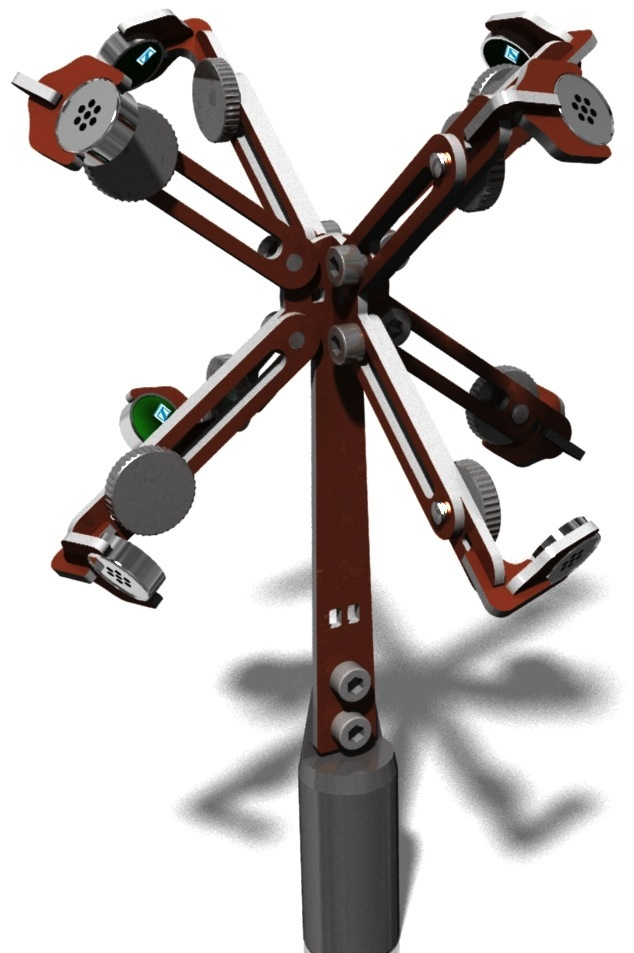
\includegraphics[width=\textwidth]{images/02_Konzeptionierung/3D_Konstruktion_Array_ohne_Kanten}
                \caption{3D Konstruktion}
                \label{fig:3D_Konstruktion_Array_ohne_Kanten}
        \end{subfigure}
        ~ %add desired spacing between images, e. g. ~, \quad, \qquad etc.
          %(or a blank line to force the subfigure onto a new line)
        \begin{subfigure}[b]{0.47\textwidth}
                \centering
                \includegraphics[width=\textwidth]{images/02_Konzeptionierung/Array_gefertigt}
                \caption{gefertigtes Array}
                \label{fig:Array_gefertigt}
        \end{subfigure}
        \caption{Vergleich zwischen 3D Konstruktion und Fertigungsergebnis}
        \label{fig:Vergleich_array_gefertigt}
\end{figure}
% ----------------------------------------- SUB-FIGURE ----------------------------------- 









% ****************************************************************************************
\section{Simulation}
\label{sec:Simulation}
% ****************************************************************************************
Zur Verifikation des in \Sec{sec:AnnahmenUndMatheZusammenhaenge} dargestellten mathematischen Modells wird eine umfangreiche Simulation in \matlab erstellt. Bezüglich der späteren Echtzeitimplementierung ist es notwendig, alle nötigen Programmfunktionen so zu erstellen, dass diese ebenfalls mit der zur Verfügung stehenden DSP- und C-Bibliothek umgesetzt werden können. Obwohl die Simulation nicht echtzeitkritisch ist, soll die Erfüllung des Echtzeitkriteriums bereits hier einen zentralen Punkt darstellen. Die Simulation beinhaltet folgende Komponenten:

\begin{enumerate}
    \item Ermittlung systembedingter Parameter %(wie \zB Winkelauflösung, Signalblocklänge, \dots)
    \item Erstellung synthetischer Signale
    \item Kreuzkorrelation unter Verwendung der FFT
    \item Algorithmus zur Berechnung des MCCC
    \item Optimierungsverfahren zur Ergebnis- und Geschwindigkeitsverbesserung
\end{enumerate}


% ***************************************************************************************
\subsection{Systemparameter}
\label{subsec:Systemparameter}
% ****************************************************************************************
Im Folgenden werden alle systembedingten Parameter ermittelt. Diese sind

\begin{itemize}
    \item Winkelauflösung inkl. Validierung des Winkelraums
    \item Anzahl abzusuchender Richtungen
    \item Signalblocklänge
    \item Anzahl der Kreuzkorrelationen
\end{itemize}





% ****************************************************************************************
\subsubsection{Winkelauflösung}
\label{subsubsec:Winkelaufloesung}
% ****************************************************************************************
Als grundsätzliche Anforderung an das System ist die mit der vorliegenden Hardware maximal zu erreichende Winkelauflösung abzubilden. Das heißt, je kleiner die Winkelauflösung (entspricht der Winkelschrittweite), desto größer ist die erreichbare Genauigkeit bei der Winkeldetektion. Da wie bereits erwähnt ein diskretes System realisiert wird, können nur Laufzeiten gemessen werden, die einem ganzzahligen Vielfachen der Abtastperiode $T_a$ entsprechen. Auf Grund dessen wird im Folgenden die Laufzeitdifferenz als SDOA\footnote{Sample Difference of Arrival} bezeichnet. Durch diese Zeitrasterung entsteht ebenfalls eine Winkelrasterung im Abstand der Winkelschrittweite, wodurch ein direkter Zusammenhang zwischen Winkelauflösung und verwendeter Systemabtastrate entsteht. Auf Grund der äquidistanten Anordnung benachbarter Sensoren ist die Winkelauflösung $\alpha_{\phi, \theta}$ für Azimuth- und Elevationswinkel identisch. $\alpha_{\phi, \theta}$ kann unter Verwendung von \Eq{ULA_1} und $d=d_{min}$ errechnet werden. $d_{min}$ beschreibt dabei die minimale Distanz zwischen zwei Mikrofonen. Durch Hinzufügen der Abtastperiode $T_a$ folgt $\alpha_{\phi, \theta}$ mit  


\begin{equation}
    \alpha_{\phi, \theta} = \frac{\pi}{2} - \arccos{\left( 1 \cdot T_a \cdot \frac{c}{d_{min}} \right)} 
\end{equation}

Der kleinste zu erreichende Winkelschritt hängt also direkt mit der kleinsten messbaren Laufzeitdifferenz von $1 \cdot T_a$ zusammen. \tab{Winkelaufloesung_Abtastfrequenz} zeigt mögliche Winkelauflösungen bei den im Audiobereich üblichen Abtastfrequenzen.



\begin{table}[h]
     \center
     \begin{tabular}{cc}
     \hline
          Abtastfrequenz [kHz] & Winkelauflösung [°] \\
           \hline \hline
          8                    & 47,9      \\
          16                   & 21,8      \\
          24                   & 14,3      \\
          48                   & 7,1       \\
          96                   & 3,5       \\
         \hline
     \end{tabular}
  \caption{Winkelauflösung bei unterschiedlichen Abtastfrequenzen}
 \label{tab:Winkelaufloesung_Abtastfrequenz}
 \end{table}



% ****************************************************************************************
\subsubsection{Validierung des Winkelraums} 
% ****************************************************************************************
Zur Validierung des abzubildenden Winkelraums ist es notwendig, jede mögliche Kombination aus Azimuth- und Elevationswinkel nachzumessen. Dazu wird ein Simulationsskript erstellt, das in Abhängigkeit vom eingestellten Winkelpaar den mittleren quadratischen Fehler $e_{rms}$ berechnet. Dieser ist geeignet, um die Abweichung eines Schätzers von dem zu schätzenden Wert zu ermitteln. Da die Schätzung jeder Richtung jeweils zwei Winkel liefert, werden die Fehler zunächst getrennt ermittelt. 

Der Fehler $e_{\phi | rms}$ für den Elevationswinkels $\phi$ ist gegeben durch


\begin{equation}\label{eq:rms_error_phi}
    e_{\phi | rms} = \sqrt{\frac{1}{M-1} \sum_{n=0}^{M-1} \vert \hat \phi_n - \phi \vert^2}.
\end{equation}


Für den Fehler $e_{\theta | rms}$ des Azimuthwinkel $\theta$ folgt so


\begin{equation}\label{eq:rms_error_theta}
    e_{\theta | rms} = \sqrt{\frac{1}{M-1} \sum_{n=0}^{M-1} \vert \hat \theta_n - \theta \vert^2}.
\end{equation}


Durch bilden des arithmetischen Mittelwerts resultiert der Gesamtfehler pro Richtung $\bar e_{\theta, \theta | rms}$ durch
\begin{equation}\label{eq:rms_error_phi_mid}
    \bar e_{\phi, \theta | rms} = \frac{e_{\phi | rms} + e_{\theta | rms}}{2}.
\end{equation}


\abb{algo_angle_error} zeigt das Flussdiagramm des Validierungsalgorithmus. Hier erfolgt die Wertvalidierung in einer dreifach geschachtelten Schleife. Für jedes Winkelpaar wird der gleiche Signalblock verwendet und in $M$ Unterblöcke geteilt. Diese werden alle entsprechend dem gewählten Winkelpaar synthetisch verzögert und nacheinander dem MCCC-Algorithmus zugeführt. Die Ergebnisse werden entsprechend den oben genannten Gleichungen verarbeitet und gespeichert. Der Algorithmus endet, wenn alle möglichen Winkelkombinationen durchlaufen wurden.


\myFigure{real}                  % Figure tag (missing, real)
         {veryVerySmall}                 % Size (small,medium,big)
         {h!}             % z.B. htbp
         {Algorithmus zur Validierung des abzubildenden Winkelraums}                % Figure title
         {algo_angle_error}                % Figure label 
         {02_Konzeptionierung/algo_angle_error}     % Path to real figure





\abb{angle_error} zeigt den Winkelfehler $e_{\phi | rms}$, $e_{\theta | rms}$ sowie $\bar e_{\theta, \theta | rms}$ in Abhängigkeit beider Raumwinkel. Als Quellensignal dient mittelwertfreies bandbegrenztes weißes Rauschen, mit einer Bandbreite von $B_{Noise} = 2700Hz$ im Bereich $300 Hz \leq f_{Noise} \leq 3000Hz$. Jeder Winkel wird mit einer Anzahl von $M=100$ Durchläufen simuliert. Die Auswertung der Fehlerkurven ergibt einen maximalen Fehler von:

\begin{equation*}
    \begin{array}{lll}
        e_{\phi | max} & = \displaystyle\max_{\phi,\theta}{ e_{\phi | rms}} & = 0,05° \\
        e_{\theta | max} & = \displaystyle\max_{\phi,\theta}{ e_{\theta | rms}} & = 0,4° \\
        \bar e_{\phi, \theta | max} & = \displaystyle\max_{\phi,\theta}{  \bar e_{\phi, \theta | rms}} & = 0,25°
    \end{array}
\end{equation*}

Auf Grund der sehr geringen Fehlerwerte kann davon ausgegangen werden, dass der Winkelraum innerhalb unter Berücksichtigung der Winkelschrittweite fehlerfrei abgebildet werden kann.


% OLD AND WRONG

%Zur Untersuchung des abzubildenden Winkelraums werden die Bereiche für den Elevationswinkel $\phi$ und den Azimuthwinkel $\theta$ getrennt betrachtet. \abb{AngleRes_Azimuth} zeigt die erreichbaren diskreten Laufzeitdifferenzen des Elevationswinkel über den gesamten Winkelraum. Betrachtet wurden hier die beiden untereinander liegenden Mikrofone $M_1$ und $M_5$ welche parallel zur Y-Achse positioniert sind. Analog zu \citet[S. 38]{Master_Array_Pikora} wirkt sich der Verlauf der Sinus-Funktion auf die zu erreichenden Winkel aus da die Steigung in Richtung $\frac{\pi}{2}$ \bzw $-\frac{\pi}{2}$ nicht-linear abnimmt. Bei den hier gegebenen Arrayabmaßen kann ein Winkelbereich von $-70° < \phi < 70°$ abgebildet werden. Da der Azimuthwinkel $\theta$ die Y-Achse rotiert bleibt er über den gesamten Bereich linear da sich bezüglich des betrachteten Mikrofonpaars keine Laufzeitdifferenz ergibt.

%\myFigure{real}                  % Figure tag (missing, real)
%         {medium}                 % Size (small,medium,big)
%         {position}             % z.B. htbp
%         {$K_{\phi}(\phi,\theta)$ zwischen Mikrofon $M_1$ und $M_5$ in Abhängigkeit von Azimuth- und Elevationswinkel bei einer Abtastfrequenz von $f_a = 48 kHz$}                % Figure title
%         {AngleRes_Azimuth}                % Figure label 
%         {02_Konzeptionierung/AngleRes_M1_M5}     % Path to real figure




 % ----------------------------------------- SUB-FIGURE -----------------------------------
\begin{figure}
        \centering
        \begin{subfigure}[b]{0.48\textwidth}
                \centering
                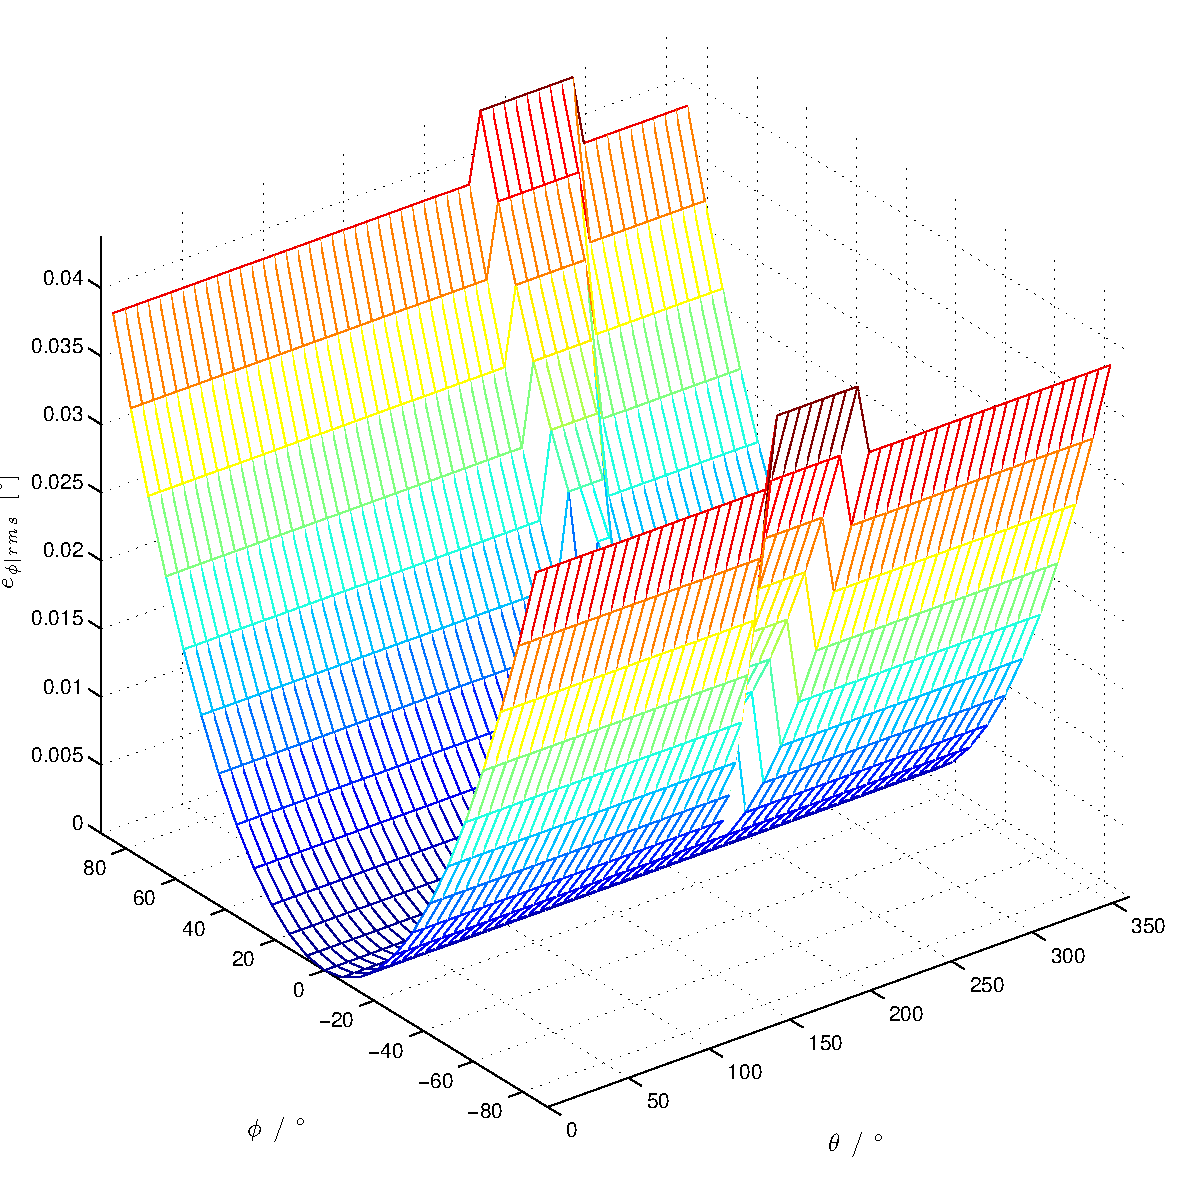
\includegraphics[width=\textwidth]{images/02_Konzeptionierung/angle_error_phi}
                \caption{$e_{\phi | rms}$}
                \label{fig:angle_error_phi}
        \end{subfigure}
        ~ %add desired spacing between images, e. g. ~, \quad, \qquad etc.
          %(or a blank line to force the subfigure onto a new line)
        \begin{subfigure}[b]{0.48\textwidth}
                \centering
                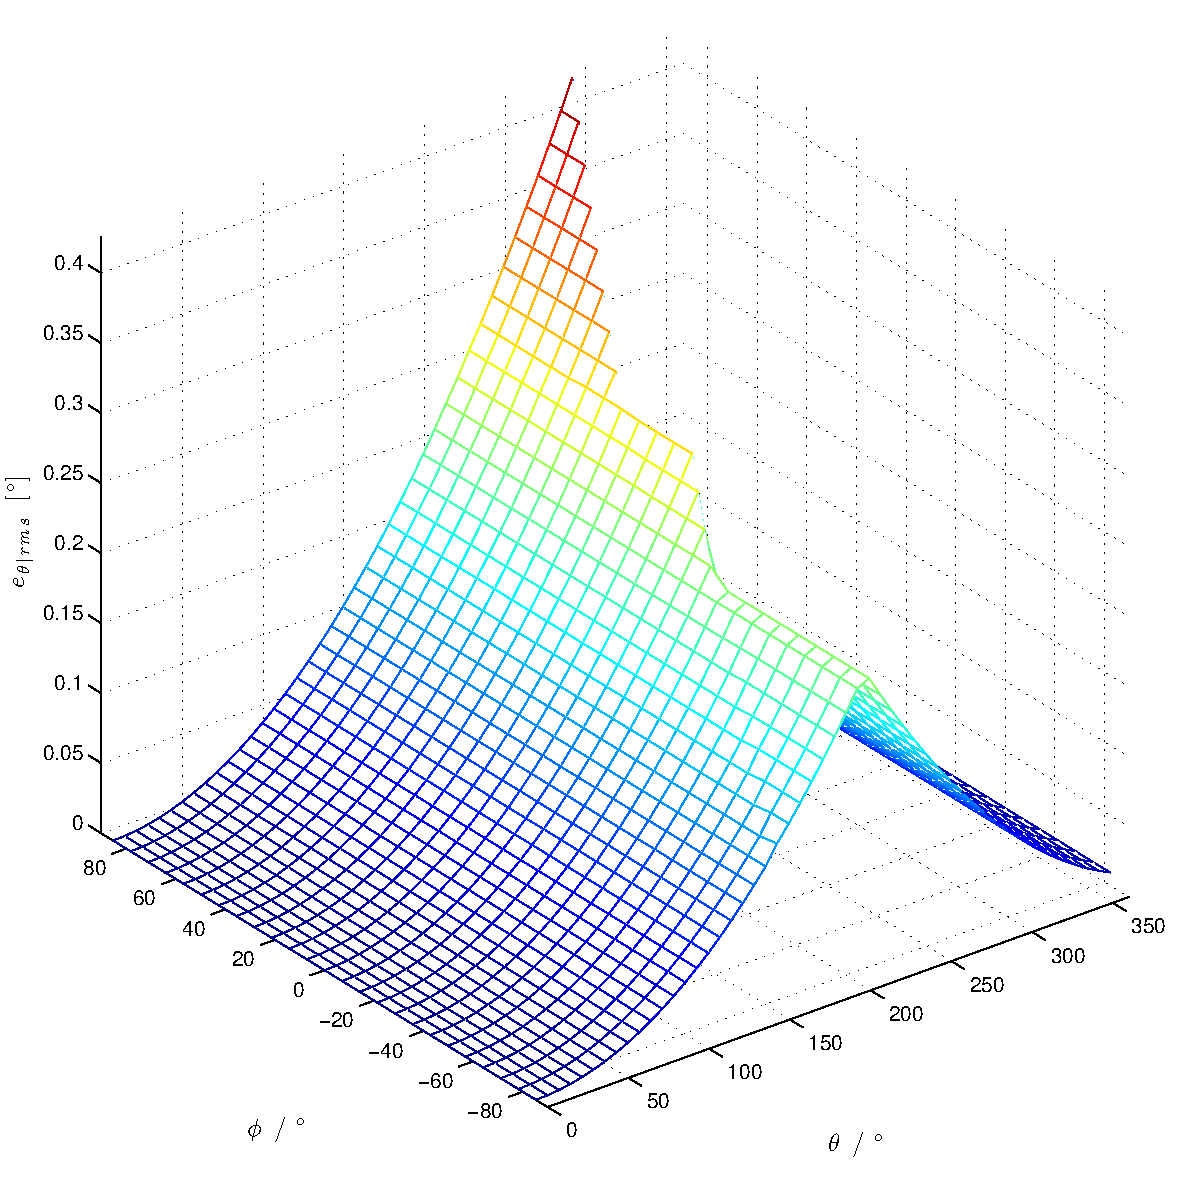
\includegraphics[width=\textwidth]{images/02_Konzeptionierung/angle_error_theta}
                \caption{$e_{\theta | rms}$}
                \label{fig:angle_error_theta}
        \end{subfigure}
        ~ %add desired spacing between images, e. g. ~, \quad, \qquad etc.
          %(or a blank line to force the subfigure onto a new line)
        \begin{subfigure}[b]{0.48\textwidth}
                \centering
                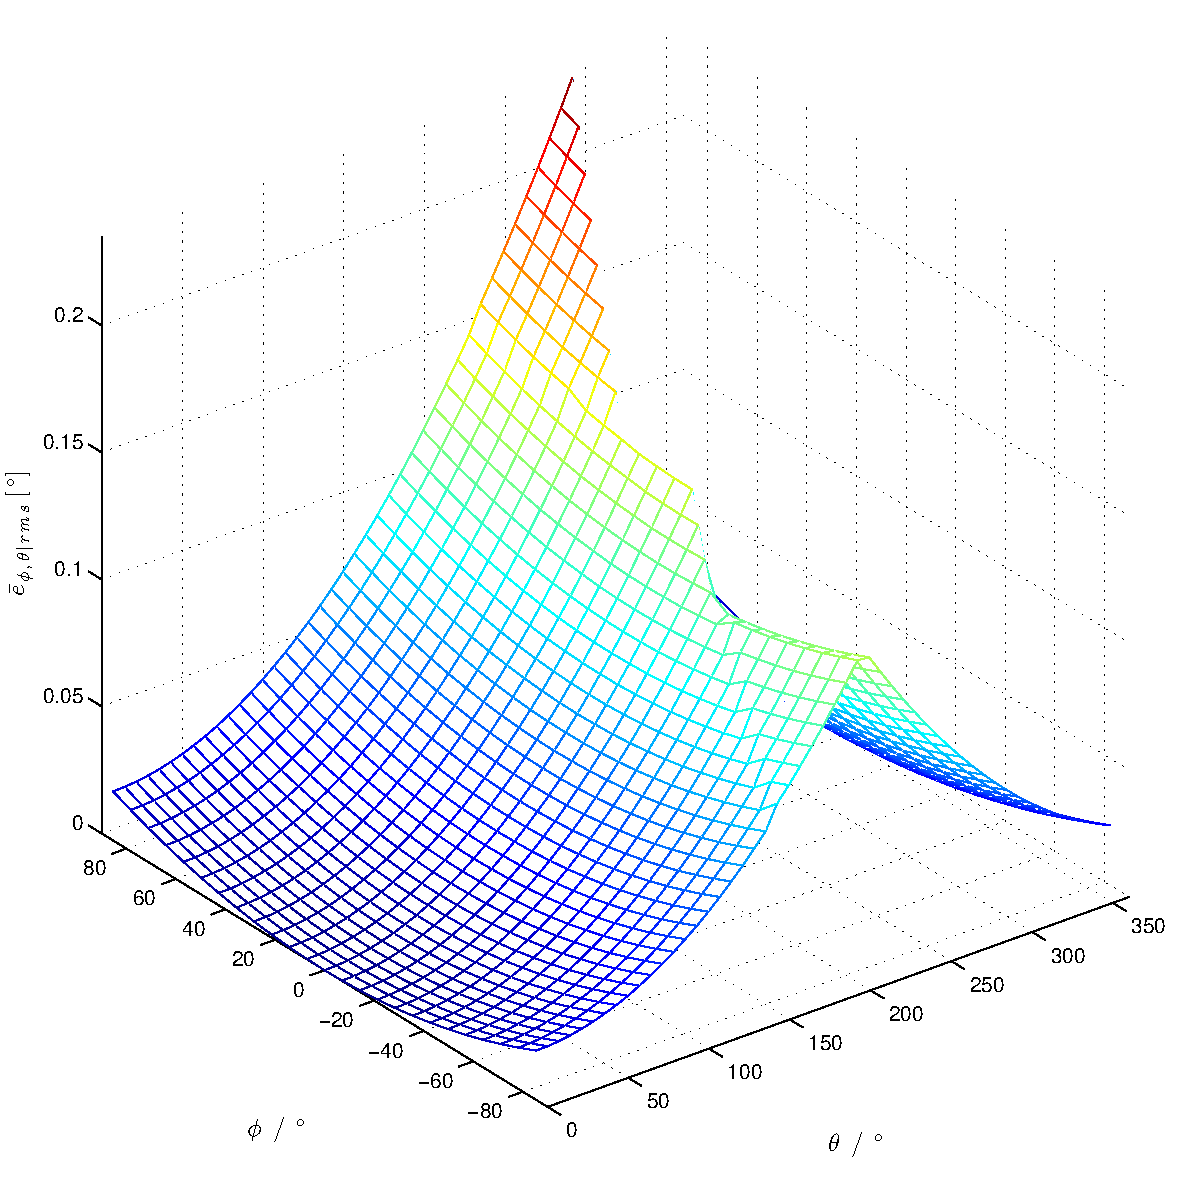
\includegraphics[width=\textwidth]{images/02_Konzeptionierung/angle_error_mid}
                \caption{$\bar e_{\phi, \theta | rms} = \frac{e_{\phi | rms} + e_{\theta | rms}}{2}$}
                \label{fig:angle_error_mid}
        \end{subfigure}
        \caption{Ergebnis der Winkelvalidierung für $e_{\phi | rms}$, $e_{theta | rms}$ und $\bar e_{\phi, \theta | rms}$ bei einer Abtastfrequenz von $f_a = 48 kHz$}
        \label{fig:angle_error}
\end{figure}
% ----------------------------------------- SUB-FIGURE ----------------------------------- 







%Zur Betrachtung des Azimuthbereiches werden die in der XY-Ebene liegenden Mikrofonpaare $M_1$ und $M_2$ (siehe \abb{AngleRes_Elevation_M12}) sowie $M_1$ und $M_4$ (siehe \abb{AngleRes_Elevation_M14}) untersucht. Die images zeigen erneut einen sinusförmigen Verlauf, nun allerdings in zwei Richtungen. Bei genauerer Betrachtung erkennt man jeweils in den Extremas der Funktion blinde Bereiche die erneut aus der abflachenden Steigung resultieren. Da die Mikrofonpaare jeweils parallel zu einer Achse der XY-Ebene verlaufen sind die Funktionen ebenfalls um $90°$ verschoben. %Da Verzögerungen zwischen diesen Mikrofonpaaren gleichzeitig gemessen und Verarbeitet werden können 

\subsubsection{Anzahl abzusuchender Richtungen}

Unter Verwendung der in \tab{Winkelaufloesung_Abtastfrequenz} angegebenen Winkelauflösungen sowie dem in \Sec{sec:Zielsetzung} genanten Winkelbereich für $\phi$ und $\theta$ ergeben sich die in \tab{Winkelanzahl_Abtastfrequenz} dargestellten Werte für die abzusuchenden Richtungen $S_{\phi,\theta}$. Der Suchaufwand wächst bei jeder Verdopplung der Abtastfrequenz überproportional an. Wie sich später zeigen wird, muss, um eine ausreichend hohe Winkelauflösung zu erreichen, ein optimiertes Suchverfahren entwickelt werden, wodurch das Echtzeitkriterium erfüllt wird. 



\begin{table}[h]
     \center
     \begin{tabular}{cccc }
     \hline
          Abtastfrequenz [kHz] & $N_{\phi}$ & $N_{\theta}$ & $S_{\phi,\theta} = N_{\phi} \cdot N_{\theta}$\\
           \hline \hline
          8                    & 4            & 8                & 32    \\
          16                   & 9            & 17               & 153    \\
          24                   & 13           & 26               & 338    \\
          48                   & 26           & 51               & 1326    \\
          96                   & 51           & 102              & 5202    \\
         \hline
     \end{tabular}
  \caption{Abzusuchende Richtungen $S_{\phi,\theta}$ bei unterschiedlichen Abtastfrequenzen}
 \label{tab:Winkelanzahl_Abtastfrequenz}
 \end{table}





%% ----------------------------------------- SUB-FIGURE -----------------------------------
%\begin{figure}
%        \centering
%        \begin{subfigure}[b]{0.48\textwidth}
%                \centering
%                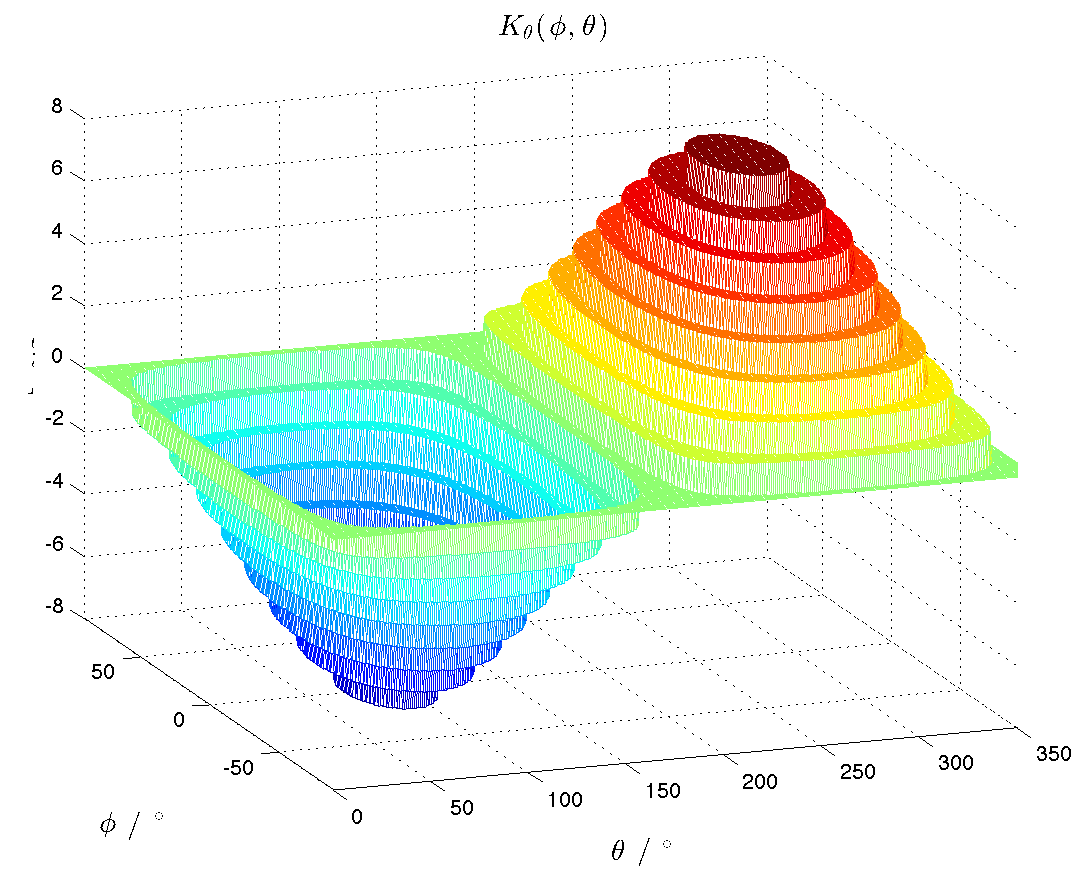
\includegraphics[width=\textwidth]{images/02_Konzeptionierung/AngleRes_M1_M2}
%                \caption{Mikrofon $M_1$ und $M_2$}
%                \label{fig:AngleRes_Elevation_M12}
%        \end{subfigure}
%        ~ %add desired spacing between images, e. g. ~, \quad, \qquad etc.
%          %(or a blank line to force the subfigure onto a new line)
%        \begin{subfigure}[b]{0.48\textwidth}
%                \centering
%                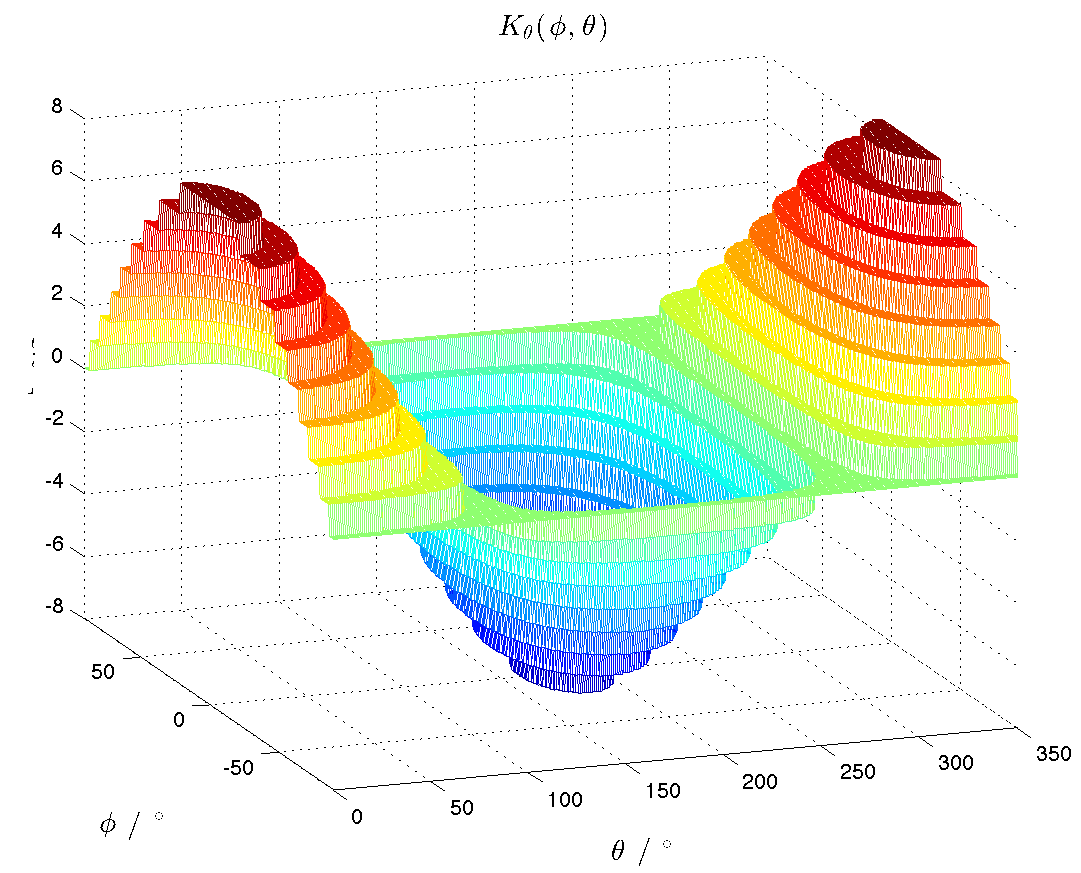
\includegraphics[width=\textwidth]{images/02_Konzeptionierung/AngleRes_M1_M4}
%                \caption{Mikrofon $M_1$ und $M_4$}
%                \label{fig:AngleRes_Elevation_M14}
%        \end{subfigure}
%        \stepcounter{missingFigureCount}
%        \caption{$K_{\theta}(\phi,\theta)$ in Abhängigkeit von Azimuth- und Elevationswinkel bei einer Abtastfrequenz von $f_a = 48 kHz$}
%        \label{fig:AngleRes_Elevation}
%\end{figure}
%% ----------------------------------------- SUB-FIGURE -----------------------------------

% ****************************************************************************************
\subsubsection{Signalblocklänge}
\label{subsubsec:Signalblocklaenge}
% ****************************************************************************************
Zum Festlegen der Signalblocklänge $L$ und somit auch der Fensterlänge $K$ der Kreuzkorrelation muss die maximale am Array messbare SDOA bestimmt werden. Diese entsteht an der hier verwendeten würfelförmigen Mikrofonanordnung genau dann, wenn der Elevationswinkel $\phi=\pm45°$ beträgt und der Azimuthwinkel $\theta$ sich im $45°$ Raster bewegt. In diesem Fall muss der Schall die Distanz $2 \cdot r$ zwischen zwei gegenüberliegenden Mikrofonen zurücklegen. Die maximale Verzögerung $K_{max}$ bezogen auf die Abtastfrequenz ergibt sich durch

\begin{equation}
    K_{max} = \frac{2r}{c} \cdot f_a
\end{equation}

\tab{Maximale_SDOA} zeigt die maximalen SDOA in Abhängigkeit verschiedener Abtastfrequenzen. 

\begin{table}[h]
     \center
     \begin{tabular}{cc}
     \hline
          Abtastfrequenz [kHz] & Maximale SDOA [Sample] \\
           \hline \hline
          8                    & $\pm$ 2      \\
          16                   & $\pm$ 5      \\
          24                   & $\pm$ 7      \\
          48                   & $\pm$ 14       \\
          96                   & $\pm$ 28       \\
         \hline
     \end{tabular}
  \caption{Maximale SDOA bei zwei gegenüberliegenden Mikrofonen}
 \label{tab:Maximale_SDOA}
 \end{table}




\myFigure{real}                  % Figure tag (missing, real)
         {medium}                 % Size (small,medium,big)
         {h!}             % z.B. htbp
         {Schalleinfallsrichtung mit der maximal messbaren Laufzeitdifferenz}                % Figure title
         {Maxinale_Laufzeit_Array}                % Figure label 
         {02_Konzeptionierung/Maximale_Laufzeit_Array}     % Path to real figure



Bei der Wahl der Signalblocklänge $L$ muss die maximale Verzögerung berücksichtigt werden. $L$ muss mindestens so groß gewählt werden, dass die maximal positive sowie maximal negative SDOA als Maximum im Korrelogramm sichtbar werden. Weiterhin sind die in \Sec{subsec:Kreuzkorrelation} genanten Kriterien im Bezug zur FFT einzuhalten. Die Signalblocklänge $L$ muss somit die halbe Länge der FFT-Länge $K$ besitzen. Weiterhin gilt für $K = 2^p$ und $p \in  \mathbb{N}^{+}$. Somit folgt für die Signalblocklänge $L = 2^{p-1}$.

% ****************************************************************************************
\subsubsection{Anzahl der Kreuzkorrelationen}
% ****************************************************************************************
Wie bereits in \Sec{subsec:MehrkanalKreuzkorrelationskoeffizient} erwähnt ist es notwendig, für die Ermittlung der Schalleinfallsrichtng die räumliche Korrelationsmatrix $\mathbf{R}_{\phi,\theta}$ zu erstellen. Dazu müssen zunächst alle nötigen Kreuzkorrelationsfunktionen berechnet werden. Anschließend werden diesen Funktionen Funktionswerte abhängig von den gewünschten Winkeln, entnommen um $\mathbf{R}_{\phi,\theta}$ zu erstellen. Da die Kreuzkorrelatinsfunktionen zwischen allen Mikrofonpaaren erstellt werden, ist deren Anzahl abhängig von der Mikrofonanzahl $N$. Auf Grund der Symmetrieeigenschaft von $\mathbf{R}_{\phi,\theta}$ müssen $\frac{N^2-N}{2}$  Kreuzkorrelationsfunktionen sowie $N$ Varianzen berechnet werden.



% ****************************************************************************************
\subsubsection{Wahl der Systemparameter}
\label{subsubsec:WahlSystemparateter}
% ****************************************************************************************
Nach der Untersuchung aller Systemparameter ist es nun notwendig, einen Satz von Parametern zu wählen, mit dem ein reales System auf einem DSP mit endlicher Rechenkapazität realisiert werden kann. Da auf Grund von Vorgaben die Anzahl der Mikrofone mit $N=8$ feststeht ergeben sich zur Berechnung $\frac{N^2-N}{2}$ = 28 Kreuzkorrelationen sowie 8 Varianzen. Ziel ist es, eine möglichst kleine Winkelauflösung zu erreichen. So wird die Abtastfrequenz des Systems mit $f_a=48kHz$ festgelegt, wodurch sich eine Winkelauflösung von $\alpha_{\phi, \theta}=7,1°$ ergibt. Nach \tab{Winkelanzahl_Abtastfrequenz} resultiert so eine Anzahl von $S_{\phi,\theta} = 1326$ abzusuchenden Richtungen, für jeweils die räumliche Korrelationsmatrix gebildet und dessen Determiante berechnet werden müssen. Auf Grund der Stationäritätseigenschaft von Sprachsignalen ist die Größe des Signalsblocks so klein wie möglich zu wählen. Gegenläufig dazu bewegt sich die benötigte Rechenzeit, welche den Wert 

\begin{equation}
    T_{calc_{max}} \leq \frac{L}{f_a} \leq L \cdot T_a
\end{equation}

nicht überschreiten darf. Die minimale Signalblocklänge beträgt bei dieser Abtastfrequenz $L=28$. In Bezug auf die DSP Implementierung wird der Signalblock auf eine Länge von $L=256$ gesetzt. Daraus ergibt sich ein Rechenfenster von $T_{calc_{max}} = 5,33ms$.



\begin{table}[h]
     \center
     \begin{tabular}{lcc}
     \hline
          Parameter & Variable & Wert \\
           \hline \hline
          Anzahl Mikrofone          & $N$                           & 8     \\
          Abtastfrequenz            & $f_a$                         & 48 kHz      \\
          Anzahl KKF                &  -                             & 28      \\
          Anzahl Varianz            &   -                            & 8       \\
          Winkelauflösung           & $\alpha_{\phi, \theta}$       & $7,1°$       \\
          Anzahl Suchrichtungen      & $S_{\phi,\theta}$             & $1326$        \\
          maximale Rechenzeit       & $T_{calc_{max}}$              & 5,33 ms         \\
         \hline
     \end{tabular}
  \caption{Gewählte Systemparameter im Überblick}
 \label{tab:Systemparameter}
 \end{table}




%\todo[inline]{Hier noch die entsprechende Abtastfrequenz wählen. Eingehen auf stationärität von Sprache (Signalblöcklänge), möglichst hohe Winkelauflösung, möglichst wenig abzusuchende Richtungen.}



% ****************************************************************************************
\subsection{Erstellung synthetischer Signale}
\label{subsec:ErstellungSynthetischerSignale}
% ****************************************************************************************
Zur Verifikation korrekter Algorithmusfunktionalität ist es notwendig, über Testsignale zu verfügen, bei denen genaue Kenntnis über die zu erwartenden Ergebnisse vorliegen. Am besten eignen sich dazu synthetisch erzeugte Signale. So lassen sich beliebige Testsignale für jede gewünschte Schalleinfallsrichtung für eine beliebige Anzahl von Mikrofonen erzeugen.

Wie in \Sec{subsec:Sensormodell} beschrieben, lassen sich zu jeder Schalleinfallsrichtung ($\phi, \theta$), bezogen auf das Referenzmikrofon, und jedem sich im Array befindenden Mikrofone jeweils eine Verzögerung zuordnen. Im Umkehrschluss kann so aus einem eindimesionalen Signalvektor ein $N+1$-Dimensionaler erzeugt werden in dem jedes der weiteren $N$ Mikrofone entsprechend einer gewünschten Schalleinfallsrichtung zeitlich verschoben wird. Diese Verschiebung kann mit dem Verschiebungssatz der Fourier-Transformation in \Eq{DFT_Verschiebung} erreicht werden, wobei der Parameter $N$ für die DFT-Länge steht \cite[S. 213]{Book_SigSys_Werner}.

\begin{equation}\label{eq:DFT_Verschiebung}
  x[n-m] \hspace{0.3cm} \overset{DFT}{\underset{N}{\longleftrightarrow}} \hspace{0.3cm} W^{mk}_N \cdot X[k]
\end{equation}

Zur Sicherstellung eines reelen Spektrums nach der Transformation kann die Symmetrieeigenschaft der Fourier-Transformation genutzt werden. Ist die Zeitfunktion gerade, d.h. $x[n] = x[-n]$, ergeben sich alle komplexen Anteile zu Null. Um dieses Verhalten auch bei ungeraden Funktionen zu erzwingen, wird die Folge an der Y-Achse gespiegelt. Nach der Multiplikation mit dem komplexen Verschiebungsterm und der Rücktransformation in den Zeitbereich können die gespiegelten Folgenelemente verworfen werden. \abb{Algo_Synthetisch_Zeitverschiebung} zeigt ein Flussdiagramm des implementierten Algorithmus. 




\myFigure{real}                  % Figure tag (missing, real)
         {small}                 % Size (small,medium,big)
         {h!}             % z.B. htbp
         {Algorithmus zur zeitlichen Verschiebung von N Signalen}                % Figure title
         {Algo_Synthetisch_Zeitverschiebung}                % Figure label 
         {02_Konzeptionierung/Algo_Synthetisch_Zeitverschiebung}     % Path to real figure




% ****************************************************************************************
\subsection{Kreuzkorrelation unter Verwendung der FFT}
\label{subsec:KreuzkorrelationVerwendungFFT}
% ****************************************************************************************
Der Ablauf zur Berechnung der $\frac{N^2-N}{2}$ Kreuzkorrelationsfunktionen sowie der $N$ Varianzen ist in \abb{Algo_CC_Var} dargestellt. Im Vergleich zur beschriebenen Mathematik in \Sec{subsec:MehrkanalKreuzkorrelationskoeffizient} werden die Sensorsignale vor der Korrelation nicht entsprechend einer Schalleinfallsrichtung zeitlich zueinander ausgerichtet. Grund hierfür ist der enorme Rechenaufwand der dadurch entstehen würde. Der Berechnungsvorgang der Kreuzkorrelation müsste in diesem Fall entsprechend der angegebenen Anzahl von Richtungen $S_{\phi,\theta}$ in \tab{Winkelanzahl_Abtastfrequenz} wiederholt werden, wodurch sich eine Echtzeitimplementierung als schwierig erweist. Da sich die Zeitverzögerung zwischen einem Signal und dessen verschobener Kopie in der Position der Kreuzkorrelationsfunktionen auf dessen Zeitachse widerspiegelt, kann die Verschiebung der Zeitsignale vor der Korrelation oder die Verschiebung des Korrelogramms nach der Korrelation um jeweils die selbe Zeit als äquivalent betrachtet werden. Unter Anwendung der Korrelogrammverschiebung kann Rechenzeit eingespart werden, da die oben angegebene Anzahl von Korrelationsoperationen nur einmal pro Signalblock berechnet werden muss.

 


%Die Berechnung der Varianzen läuft in einer einfach geschachtelten schleife ab wobei zur Ermittlung der Korrelationsfunktionen zwischen jedem Sensorpaar eine doppelt geschachtelte schleife nötig ist.




\myFigure{real}                                                   % Figure tag (missing, real)
         {veryVerySmall}                                                       % Size (small,medium,big)
         {h!}                                                  % z.B. htbp
         {Algorithmus zur Berechnung der nötigen Kreuzkorrelationsfunktionen $r_{y_i, y_j}$ sowie Varianzen $\sigma^2_{y_n}$}    % Figure title
         {Algo_CC_Var}                                               % Figure label 
         {02_Konzeptionierung/Algo_CC_Var}                           % Path to real figure

% ****************************************************************************************
\subsection{Algorithmus zur Berechnung des MCCC}
% ****************************************************************************************
\abb{Algo_MCCC} zeigt den Ablauf zur Berechnung des Mehrkanal-Kreuzkorrelationskoeffizienten. Zu Beginn wird abhängig vom Azimuth- und Elevationswinkel die räumliche Korrelationsmatrix  $\mathbf{R}_{\phi,\theta}$ gebildet. Wie bereits in \Sec{subsec:KreuzkorrelationVerwendungFFT} erwähnt, erfolgt dies durch Korrelogrammverschiebung unter Verwendung von $f_n(\phi, \theta)$ mit $\mathbf{R}_{\phi,\theta}=$

\begin{equation}
    \begin{bmatrix}
    \sigma_{y_0}^2	     & r_{y_0 y_1}(k + f_1(\phi,\theta))     & \dots & r_{y_0 y_N}(k + f_N(\phi,\theta))       \\
    r_{y_0 y_1}(k + f_1(\phi,\theta))	  & \sigma_{y_1}^2      & \dots & r_{y_1 y_N}(k + f_N(\phi,\theta) - f_1(\phi,\theta))        \\
    \vdots	            & \vdots 	           & \ddots & \vdots                \\
    r_{y_0 y_N}(k + f_N(\phi,\theta))	  & r_{y_1 y_N}(k + f_N(\phi,\theta) - f_1(\phi,\theta))     & \dots	 & \sigma_{y_N}^2
    \end{bmatrix}
\end{equation}



Anschließend erfolgt die Berechnung der Determinante, wobei dessen Wert in einem separaten zweidimensionalen Feld $det_{\phi, \theta}$ abgelegt wird. Dieser Vorgang wird entsprechend den Angaben in \tab{Winkelanzahl_Abtastfrequenz} für jede messbare Richtung wiederholt. Abschließend wird das Minimum von $det_{\phi, \theta}$ ermittelt und der entsprechenden Richtung zugeordnet.

\abb{Sim_Synthetic_dB} zeigt das Ergebnis der MCCC-Simulation mit Verwendung eines synthetisch verzögerten Sprachsignals bei zwei unterschiedlichen Schalleinfallsrichtungen sowie SNR\footnote{Signal-Rausch-Verhältnis}. Das Sprachsignal wurde dabei mit unkorreliertem weißen Rauschen entsprechend angegebenem SNR überlagert. Zu erkennen ist, dass die Richtung auch bei geringem SNR gut detektiert werden kann.



%Zu beachten ist, dass die Anzahl der Determinantenberechnung mit wachsender Winkelauflösung stark ansteigt. 

\myFigure{real}                                                   % Figure tag (missing, real)
         {veryVerySmall}                                                       % Size (small,medium,big)
         {h!}                                                  % z.B. htbp
         {Algorithmus zur Berechnung des Mehrkanal-Kreuzkorrelations-koeffizienten}    % Figure title
         {Algo_MCCC}                                               % Figure label 
         {02_Konzeptionierung/Algo_MCCC}                           % Path to real figure

       
 % ----------------------------------------- SUB-FIGURE -----------------------------------
\begin{figure}
        \centering
        \begin{subfigure}[b]{0.48\textwidth}
                \centering
                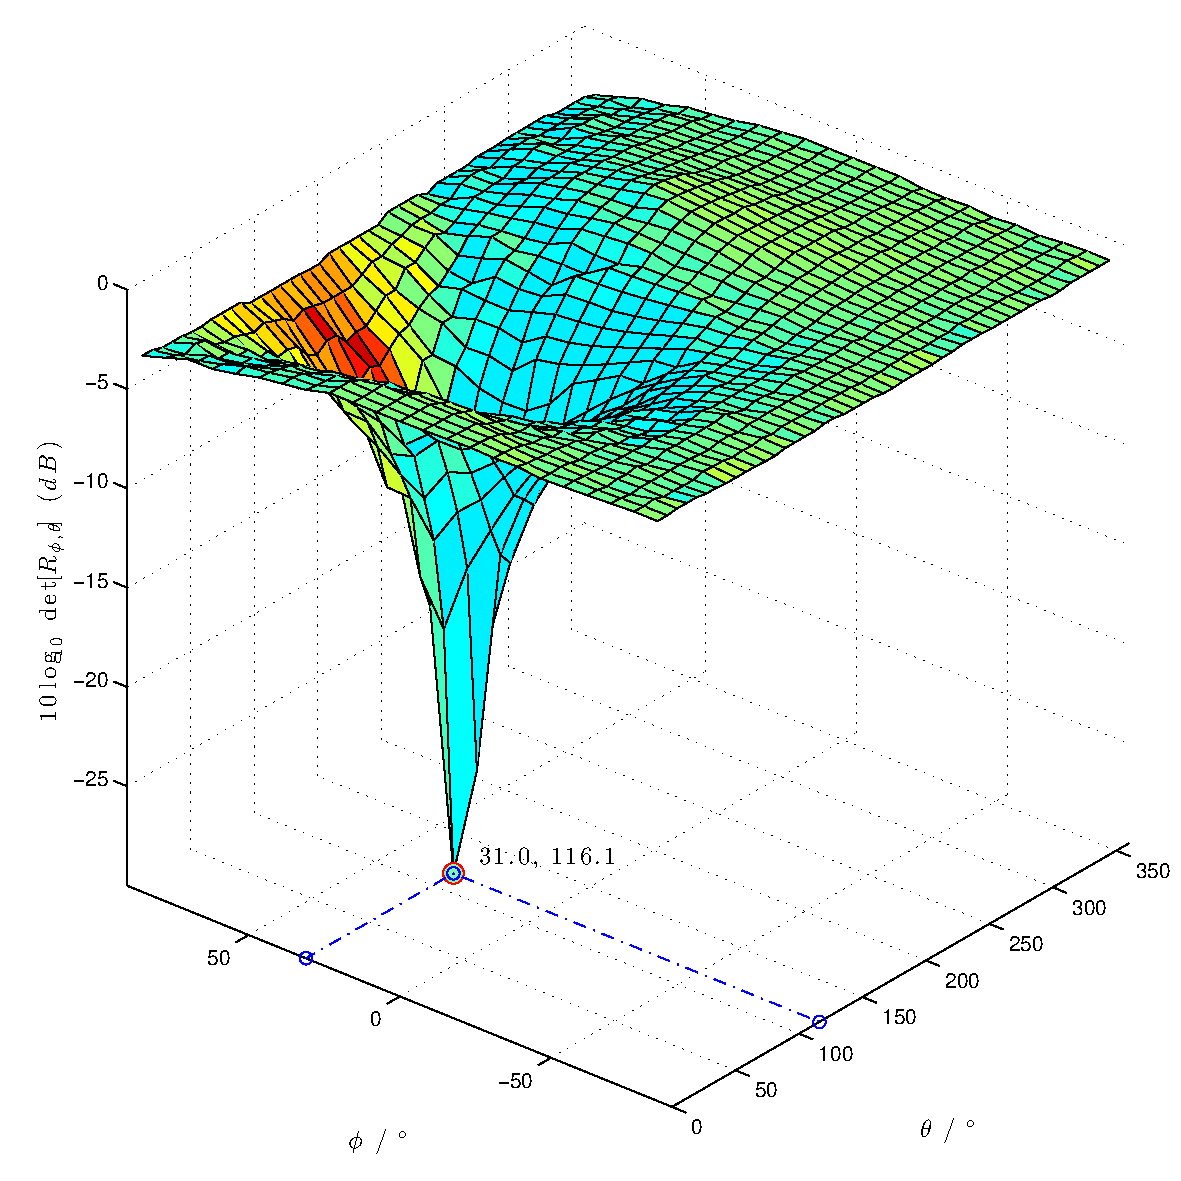
\includegraphics[width=\textwidth]{images/02_Konzeptionierung/Sim_voice_Phi_30_Theta_120_SNR_100dB_log}
                \caption{$\phi=30°,\theta=120°, \mathrm{SNR}=100dB$}
                \label{fig:Sim_Phi_30_Theta_120_dB}
        \end{subfigure}
        ~ %add desired spacing between images, e. g. ~, \quad, \qquad etc.
          %(or a blank line to force the subfigure onto a new line)
        \begin{subfigure}[b]{0.48\textwidth}
                \centering
                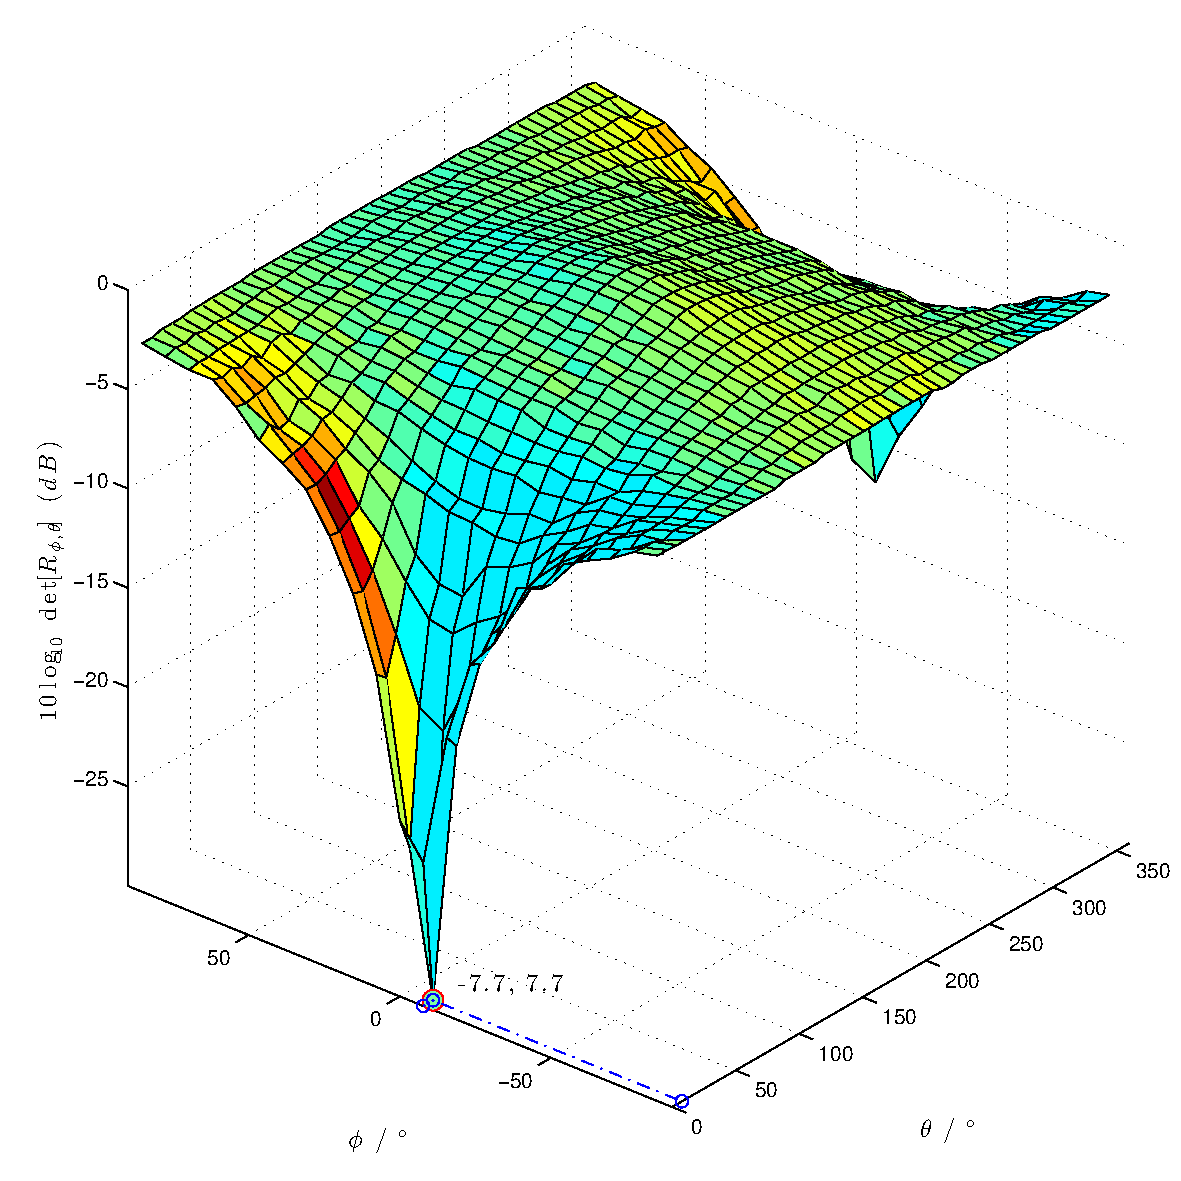
\includegraphics[width=\textwidth]{images/02_Konzeptionierung/Sim_voice_Phi_-7_Theta_7_SNR_100dB_log}
                \caption{$\phi=-7°,\theta=7°, \mathrm{SNR}=100dB$}
                \label{fig:Sim_Phi_-7_Theta_7_dB}
        \end{subfigure}
        ~ %add desired spacing between images, e. g. ~, \quad, \qquad etc.
          %(or a blank line to force the subfigure onto a new line)
        \begin{subfigure}[b]{0.48\textwidth}
                \centering
                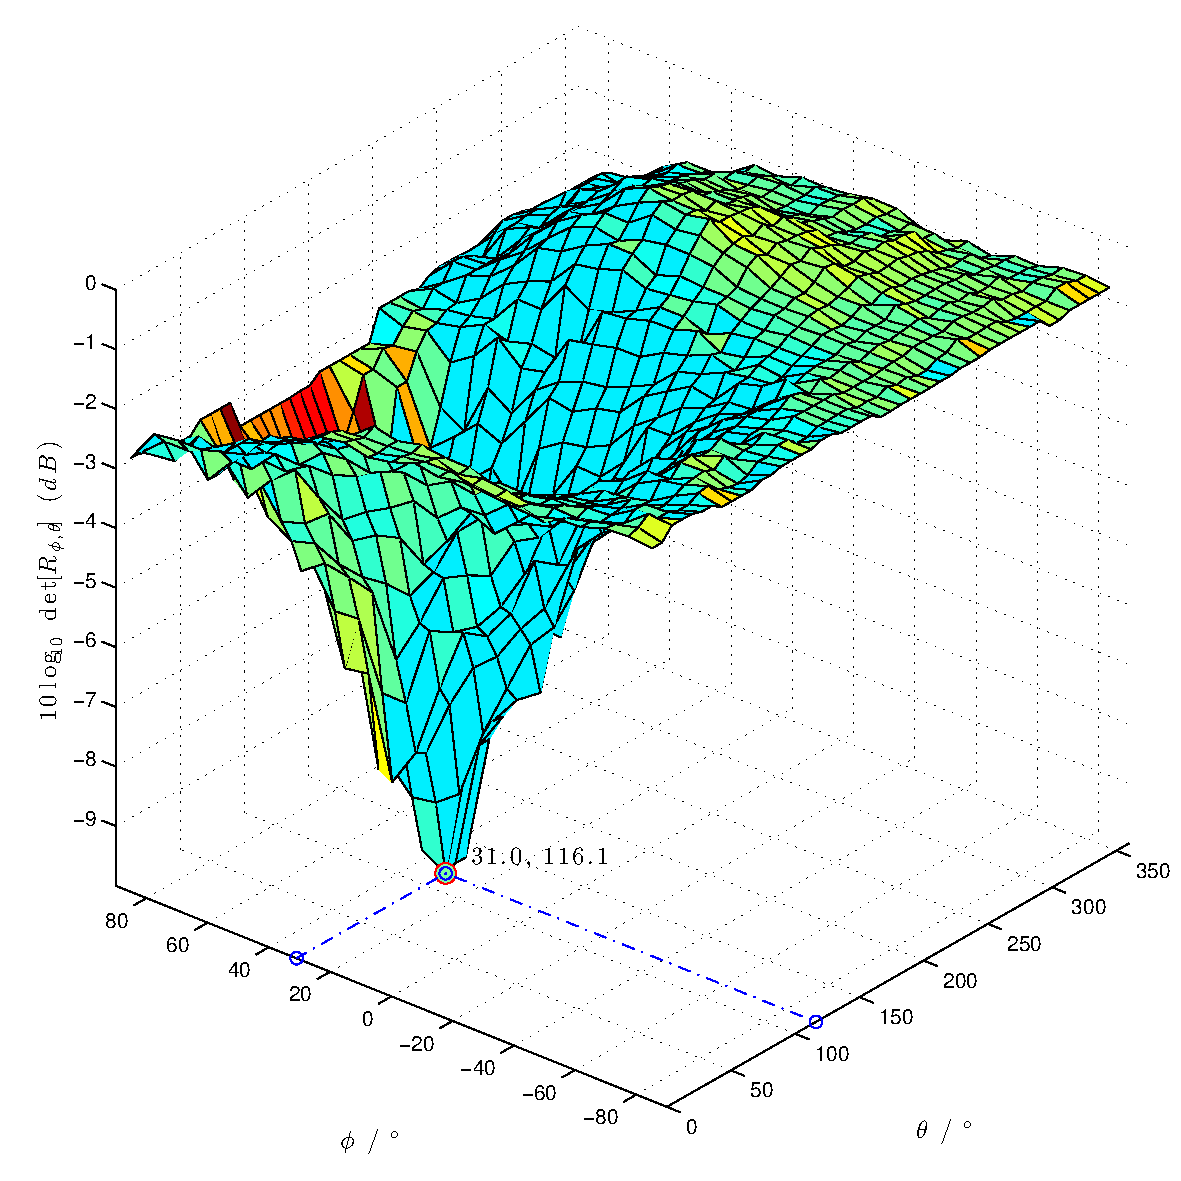
\includegraphics[width=\textwidth]{images/02_Konzeptionierung/Sim_voice_Phi_30_Theta_120_SNR_5dB_log}
                \caption{$\phi=30°,\theta=120°, \mathrm{SNR}=5dB$}
                \label{fig:Sim_Phi_30_Theta_120_dB_SNR_5dB}
        \end{subfigure}
        ~ %add desired spacing between images, e. g. ~, \quad, \qquad etc.
          %(or a blank line to force the subfigure onto a new line)
        \begin{subfigure}[b]{0.48\textwidth}
                \centering
                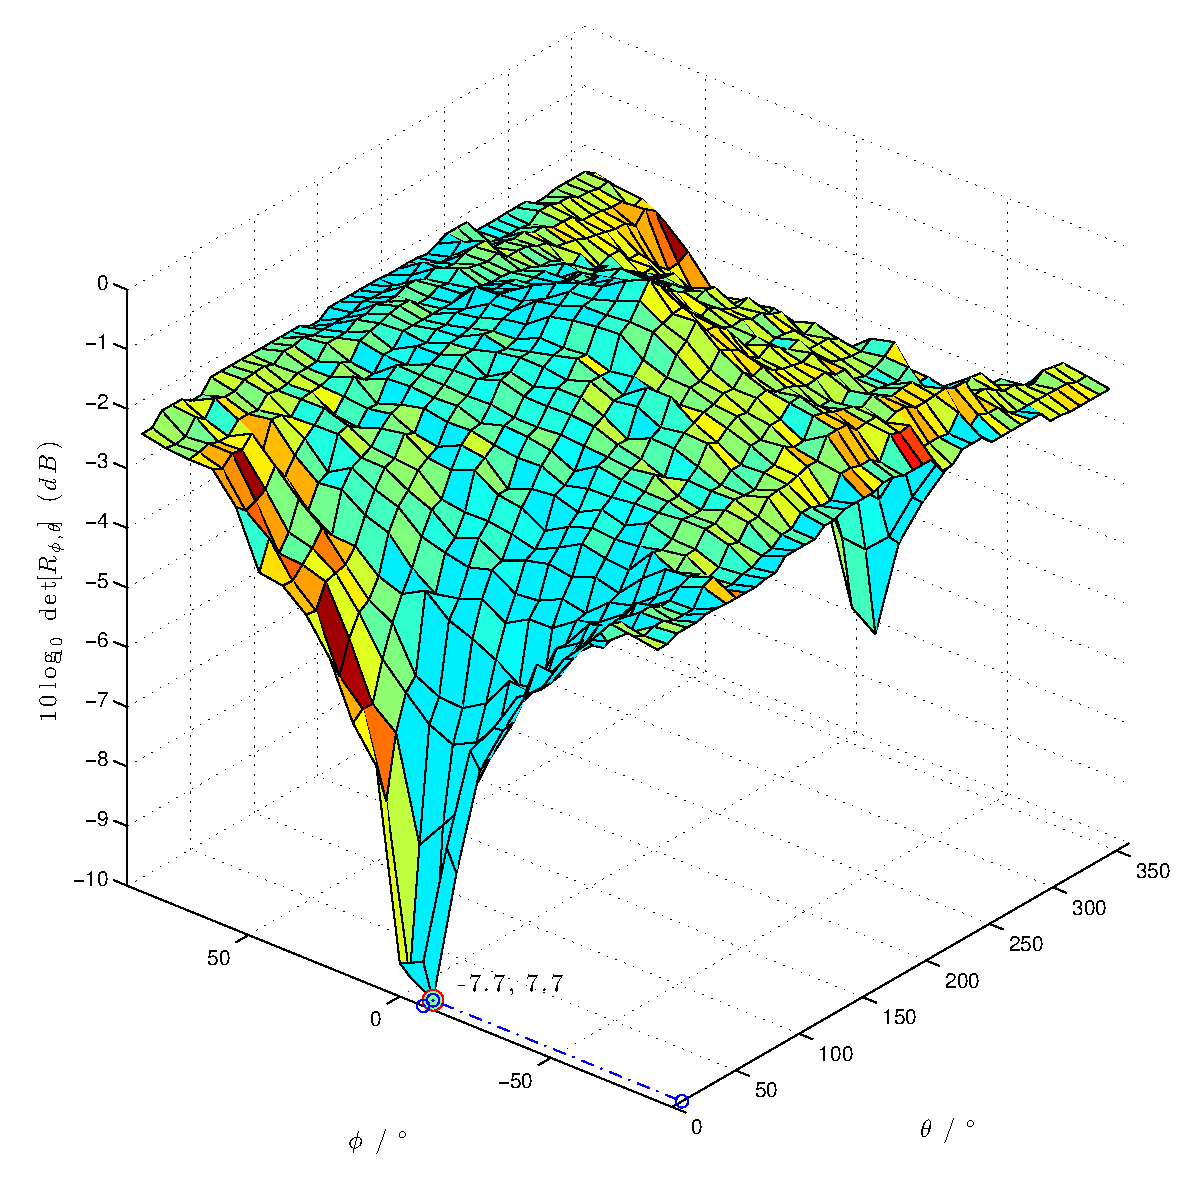
\includegraphics[width=\textwidth]{images/02_Konzeptionierung/Sim_voice_Phi_-7_Theta_7_SNR_5dB_log}
                \caption{$\phi=-7°,\theta=7°, \mathrm{SNR}=5dB$}
                \label{fig:Sim_Phi_-7_Theta_7_dB_SNR_5dB}
        \end{subfigure}
        \caption{Ergebnis des MCCC unter Verwendung eines synthetisch verzögerten Sprachsignals bei zwei unterschiedlichen Schalleinfallsrichtungen sowie SNR und einer Abtastfrequenz von $f_a=44,1kHz$.}
        \label{fig:Sim_Synthetic_dB}
\end{figure}
% ----------------------------------------- SUB-FIGURE -----------------------------------        
         
Zur Untersuchung des Korrelationsverfahrens auf die Entstehung des räumlichen Aliasing-Effekts wird die Reaktion des Systems auf ein rein periodisches Signal der Form $y[n] = \sin{\left( 2 \pi \frac{f}{f_a} n \right)}$ bei unterschiedlichen Frequenzen beobachtet. \abb{Sim_sine_spartial_aliasing} illustriert sechs Ergebnisse der MCCC im Frequenzintervall $100 Hz \leq f \leq 3kHz$. Zu sehen ist, dass sich die Ausprägung des Minimums bei steigender Frequenz deutlich verbessert. Grund hierfür ist die immer schmaler werdende Hauptkeule der Kreuzkorrelationsfunktion wie in \abb{Sim_sine_r_xy} dargestellt. Weiterhin treten in \abb{Sim_sine_spartial_aliasing} zusätzliche lokale Minima auf, deren Anzahl und Abstand von der Menge sowie Höhe der Nebenkeulen im Suchbereich (zwischen den grünen Linien in \abb{Sim_sine_r_xy}) abhängt. Bei Verletzten des Kriteriums in \Eq{raemlichesAliasing} befinden sich mehrere Spitzen innerhalb des Suchbereichs der KKF, was die Lokalisierung des korrekten Maximums erschwert. Auf Grund der hier verwendeten nicht erswartungstreuen Schätzung (siehe \Sec{subsubsec:ErwartungstreueSchaetzung}) erfährt die Kreuzkorrelation eine Gewichtung durch das Dreieckfenster, so dass die Nebenmaxima gedämpft werden und die Wahrscheinlichkeit der Entstehung von räumlichem Aliasing deutlich verringert wird.



% ----------------------------------------- SUB-FIGURE -----------------------------------
\begin{figure}
        \centering
        \begin{subfigure}[b]{0.48\textwidth}
                \centering
                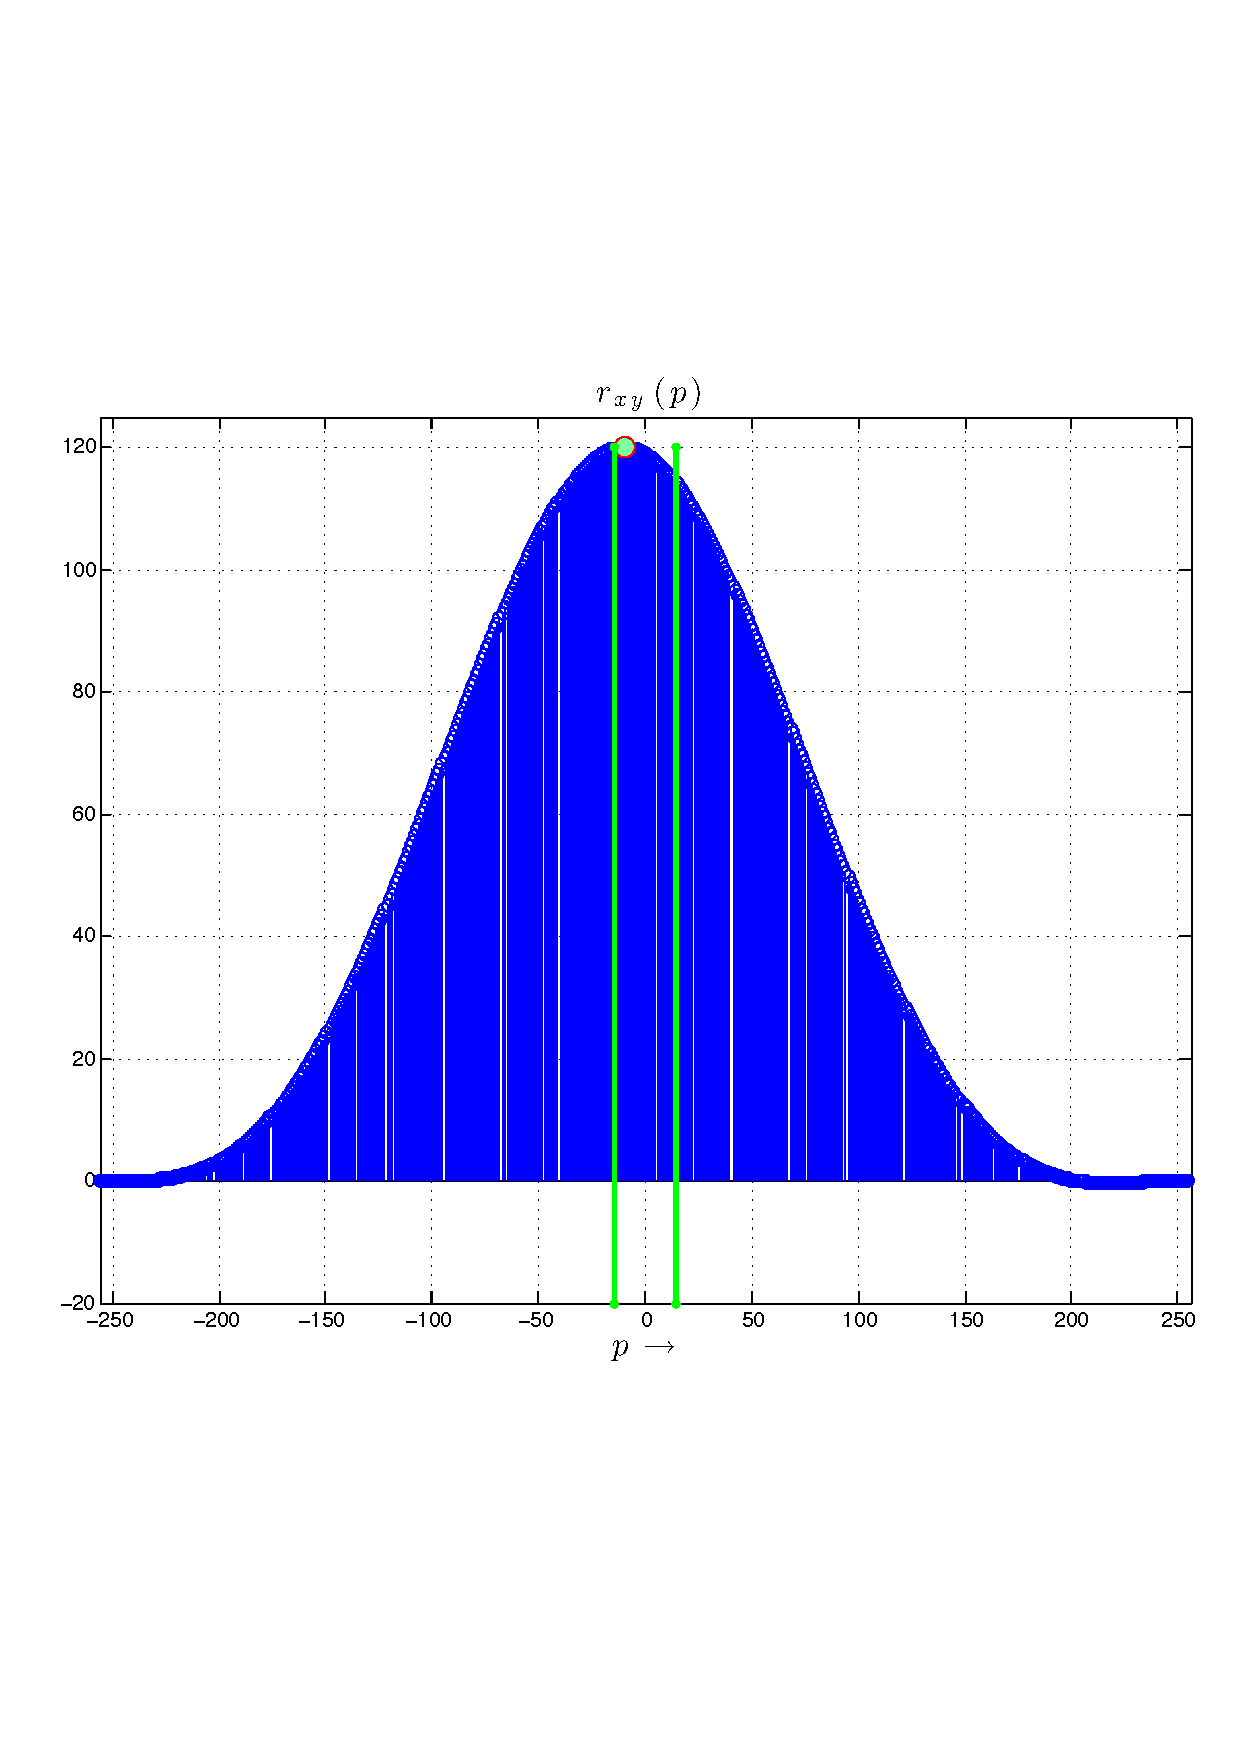
\includegraphics[width=\textwidth]{images/02_Konzeptionierung/sine_rxy_f_100}
                \caption{$f=100Hz$}
                \label{fig:sine_rxy_f_100}
        \end{subfigure}
        ~ %add desired spacing between images, e. g. ~, \quad, \qquad etc.
          %(or a blank line to force the subfigure onto a new line)
        \begin{subfigure}[b]{0.48\textwidth}
                \centering
                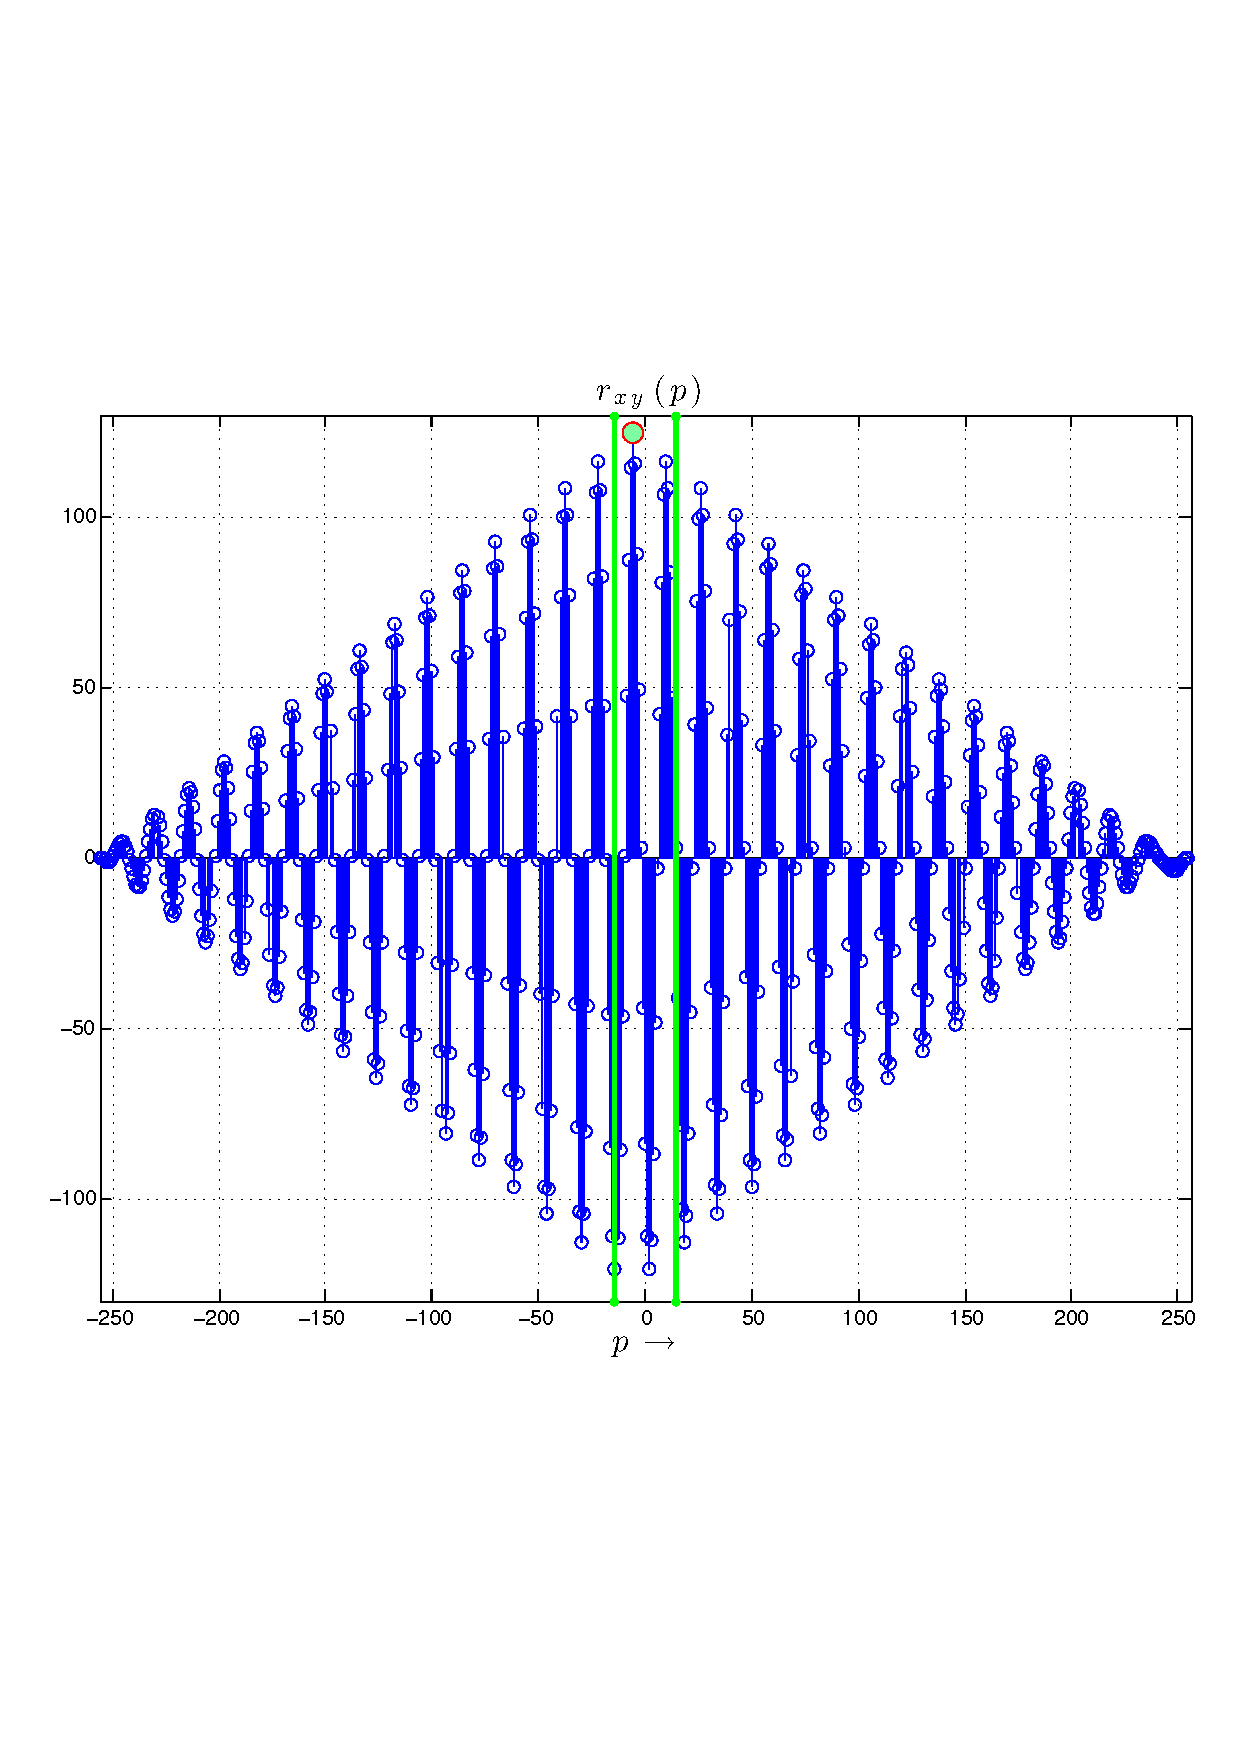
\includegraphics[width=\textwidth]{images/02_Konzeptionierung/sine_rxy_f_3000}
                \caption{$f=3000Hz$}
                \label{fig:sine_rxy_f_3000}
        \end{subfigure}
        \caption{Ergebnis der Kreuzkorrelations unter Verwendung eines synthetisch verzögerten Sinussignals bei einer Abtastfrequenz von $f_a=48kHz$.}
        \label{fig:Sim_sine_r_xy}
\end{figure}
% ----------------------------------------- SUB-FIGURE -----------------------------------

  
 % ----------------------------------------- SUB-FIGURE -----------------------------------
\begin{figure}
        \centering
        \begin{subfigure}[b]{0.48\textwidth}
                \centering
                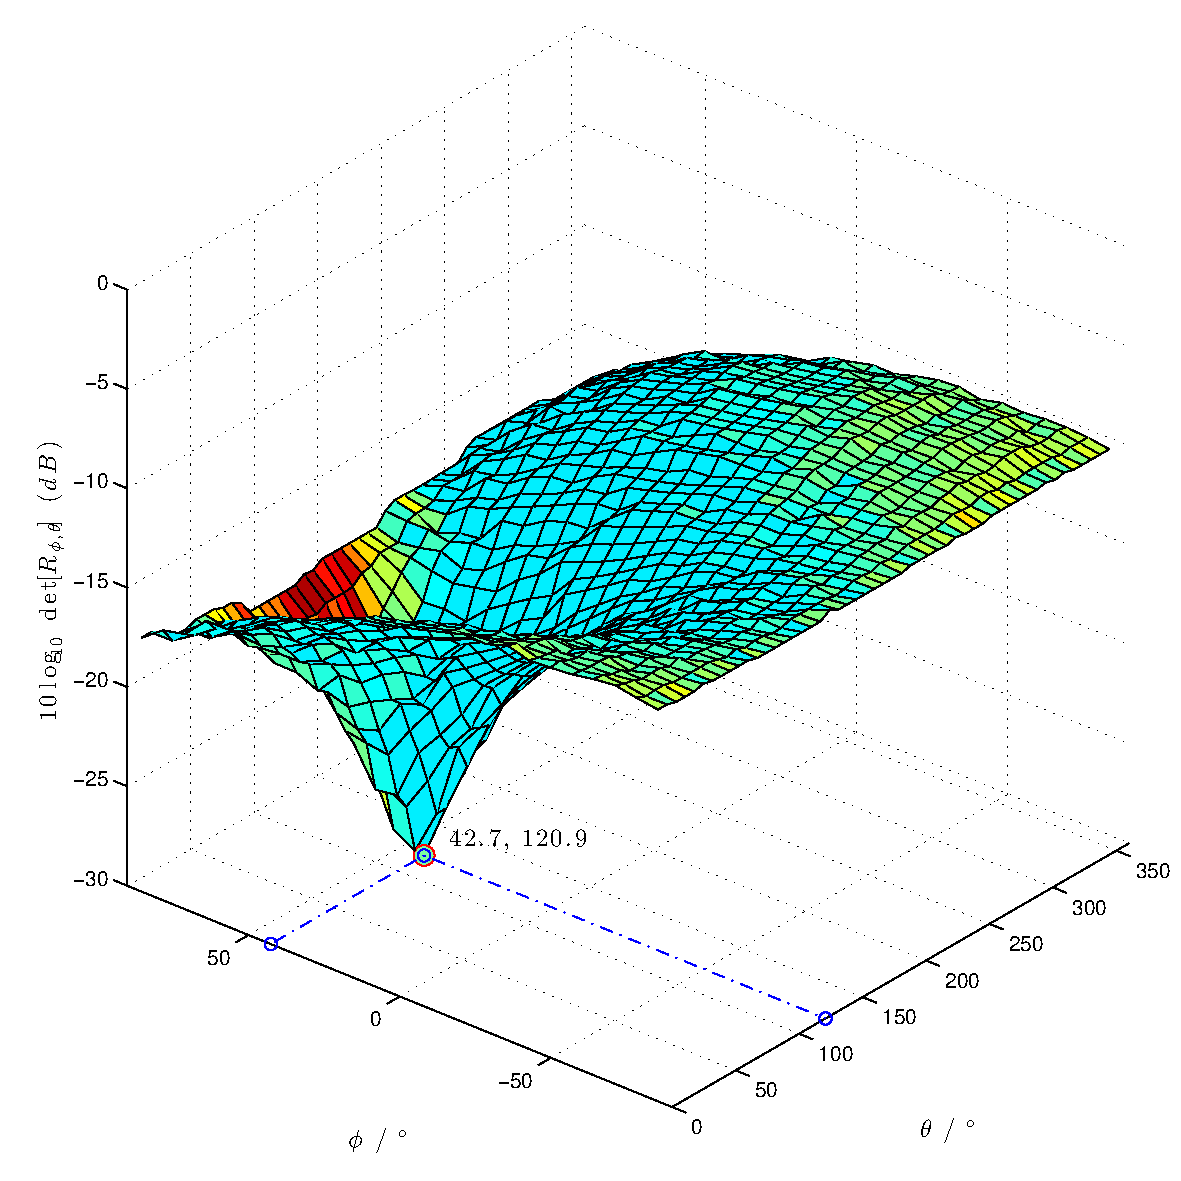
\includegraphics[width=\textwidth]{images/02_Konzeptionierung/Sim_sine_f_100_Phi_45_Theta_120_dB_SNR_100dB}
                \caption{$f=100Hz$}
                \label{fig:Sim_sine_f_100_Phi_45_Theta_120_dB_SNR_100dB}
        \end{subfigure}
        ~ %add desired spacing between images, e. g. ~, \quad, \qquad etc.
          %(or a blank line to force the subfigure onto a new line)
        \begin{subfigure}[b]{0.48\textwidth}
                \centering
                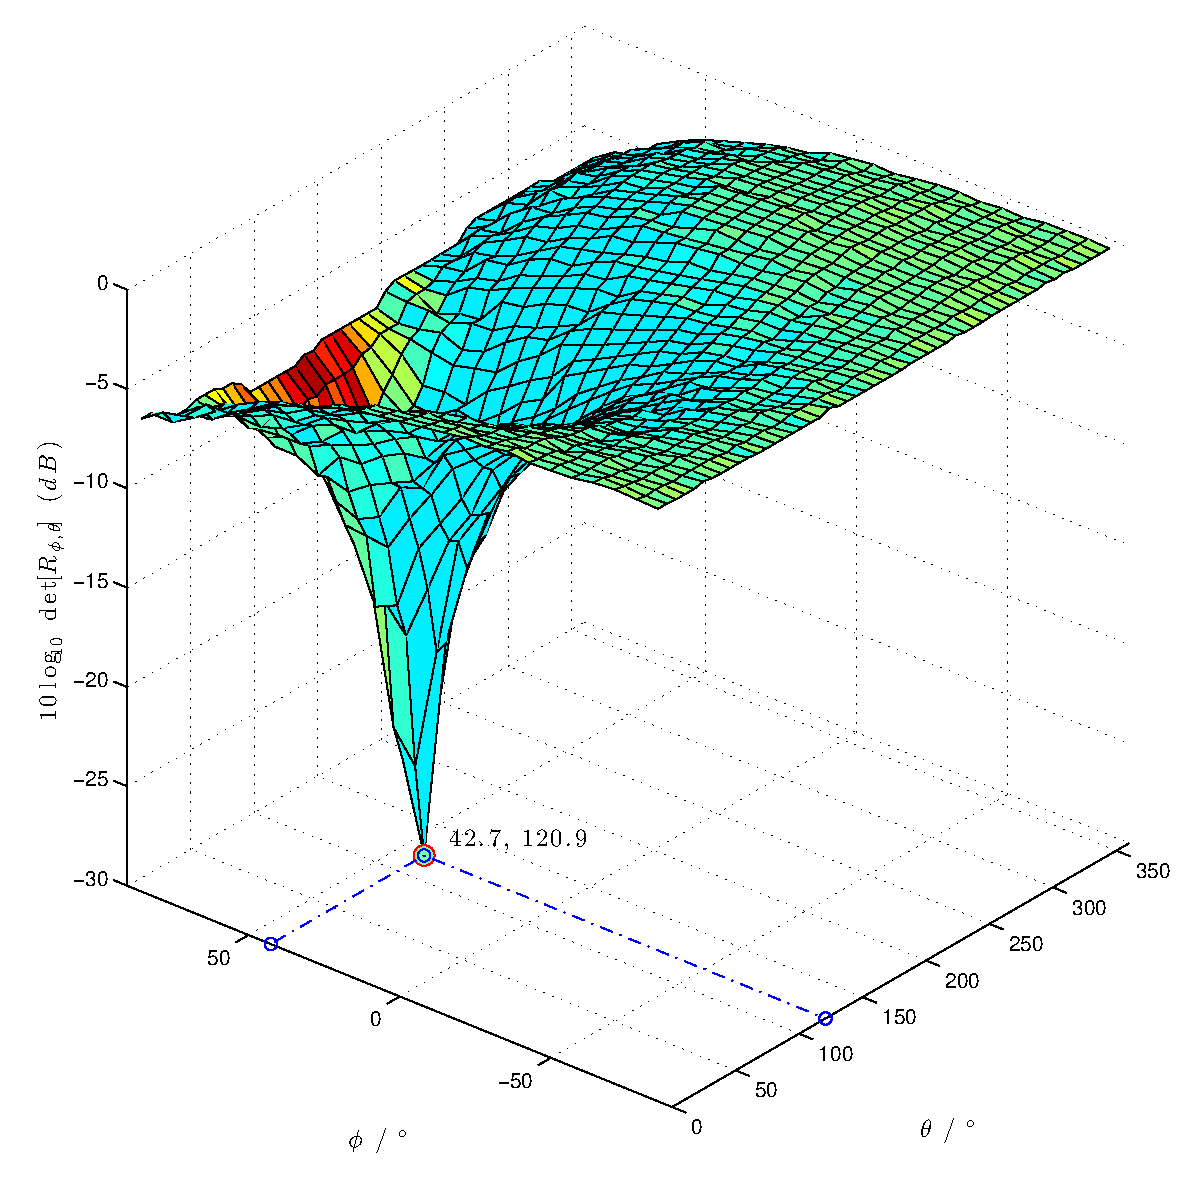
\includegraphics[width=\textwidth]{images/02_Konzeptionierung/Sim_sine_f_500_Phi_45_Theta_120_dB_SNR_100dB}
                \caption{$f=500Hz$}
                \label{fig:Sim_sine_f_500_Phi_45_Theta_120_dB_SNR_100dB}
        \end{subfigure}
        ~ %add desired spacing between images, e. g. ~, \quad, \qquad etc.
          %(or a blank line to force the subfigure onto a new line)
        \begin{subfigure}[b]{0.48\textwidth}
                \centering
                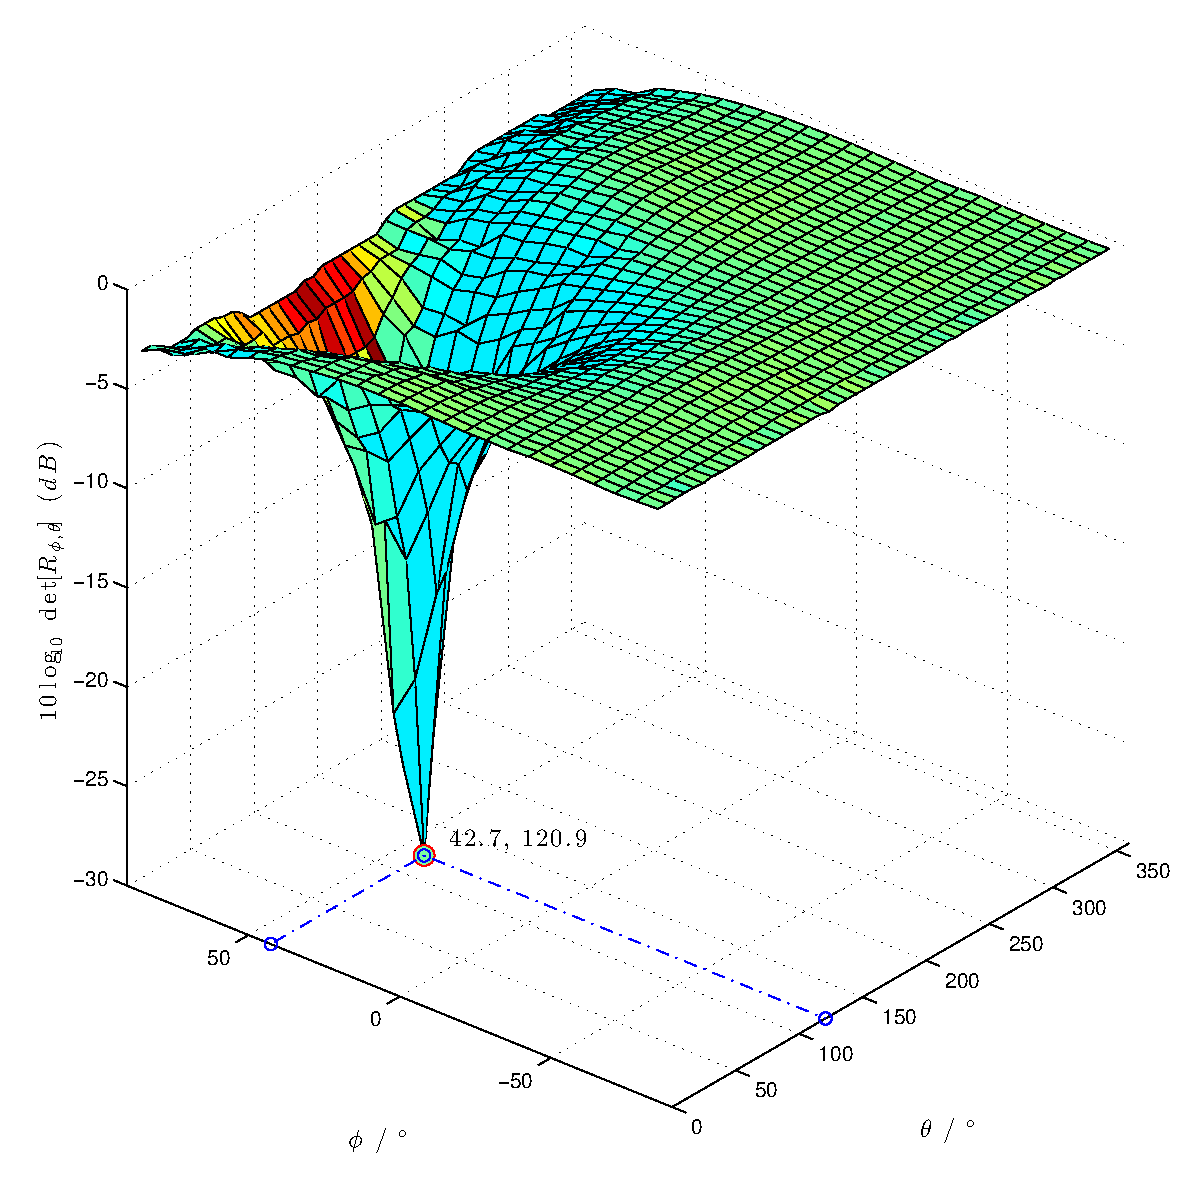
\includegraphics[width=\textwidth]{images/02_Konzeptionierung/Sim_sine_f_1000_Phi_45_Theta_120_dB_SNR_100dB}
                \caption{$f=1000Hz$}
                \label{fig:Sim_sine_f_1000_Phi_45_Theta_120_dB_SNR_100dB}
        \end{subfigure}
        ~ %add desired spacing between images, e. g. ~, \quad, \qquad etc.
          %(or a blank line to force the subfigure onto a new line)
        \begin{subfigure}[b]{0.48\textwidth}
                \centering
                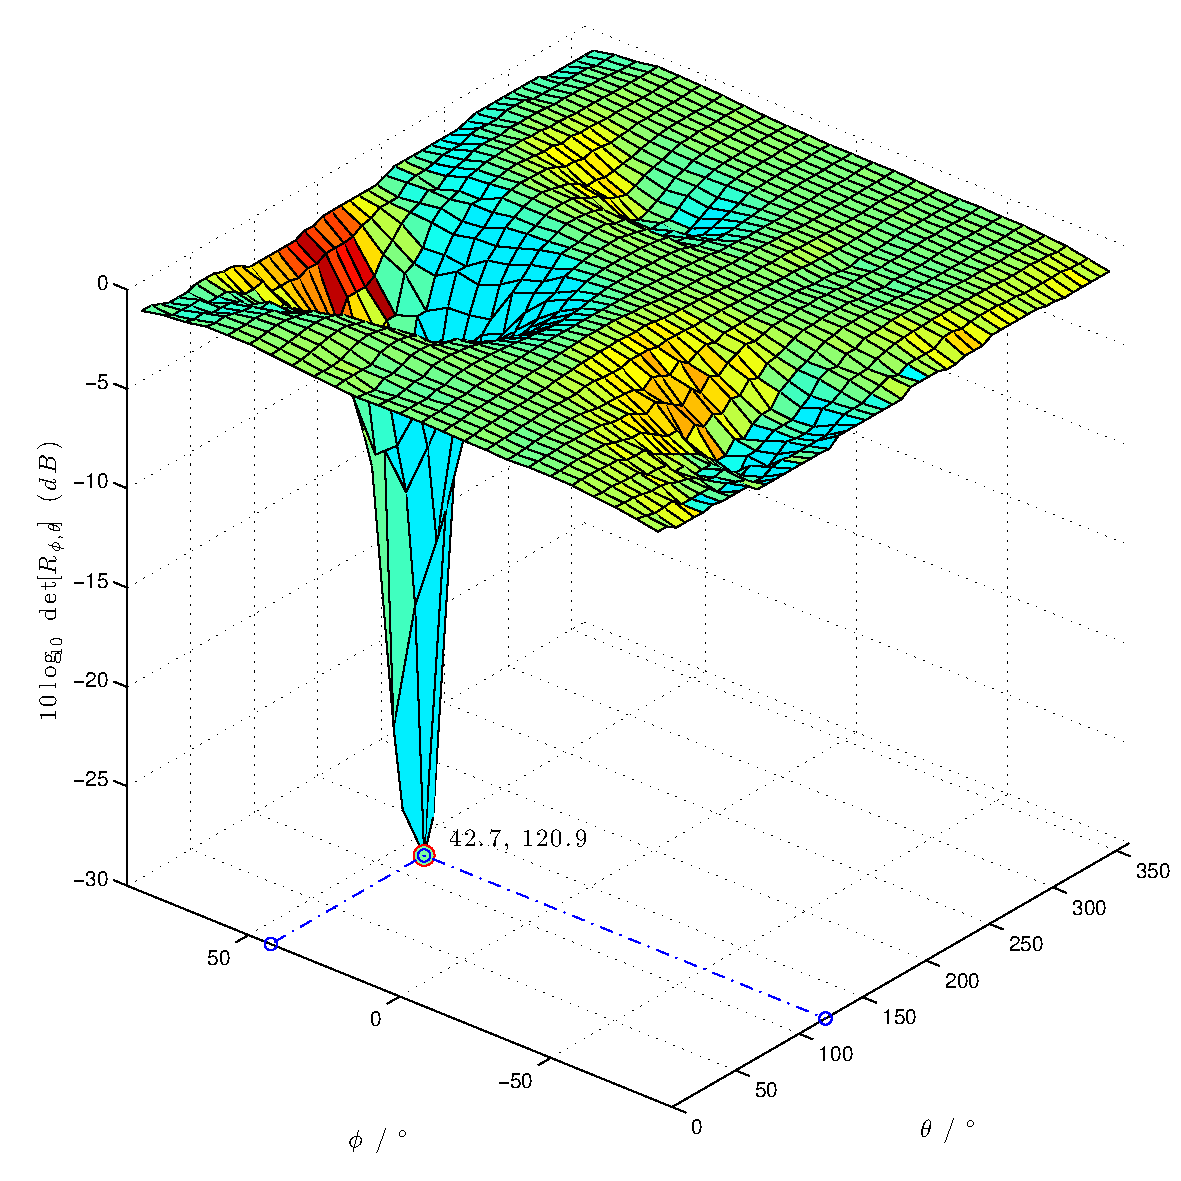
\includegraphics[width=\textwidth]{images/02_Konzeptionierung/Sim_sine_f_1500_Phi_45_Theta_120_dB_SNR_100dB}
                \caption{$f=1500Hz$}
                \label{fig:Sim_sine_f_1500_Phi_45_Theta_120_dB_SNR_100dB}
        \end{subfigure}
                ~ %add desired spacing between images, e. g. ~, \quad, \qquad etc.
          %(or a blank line to force the subfigure onto a new line)
        \begin{subfigure}[b]{0.48\textwidth}
                \centering
                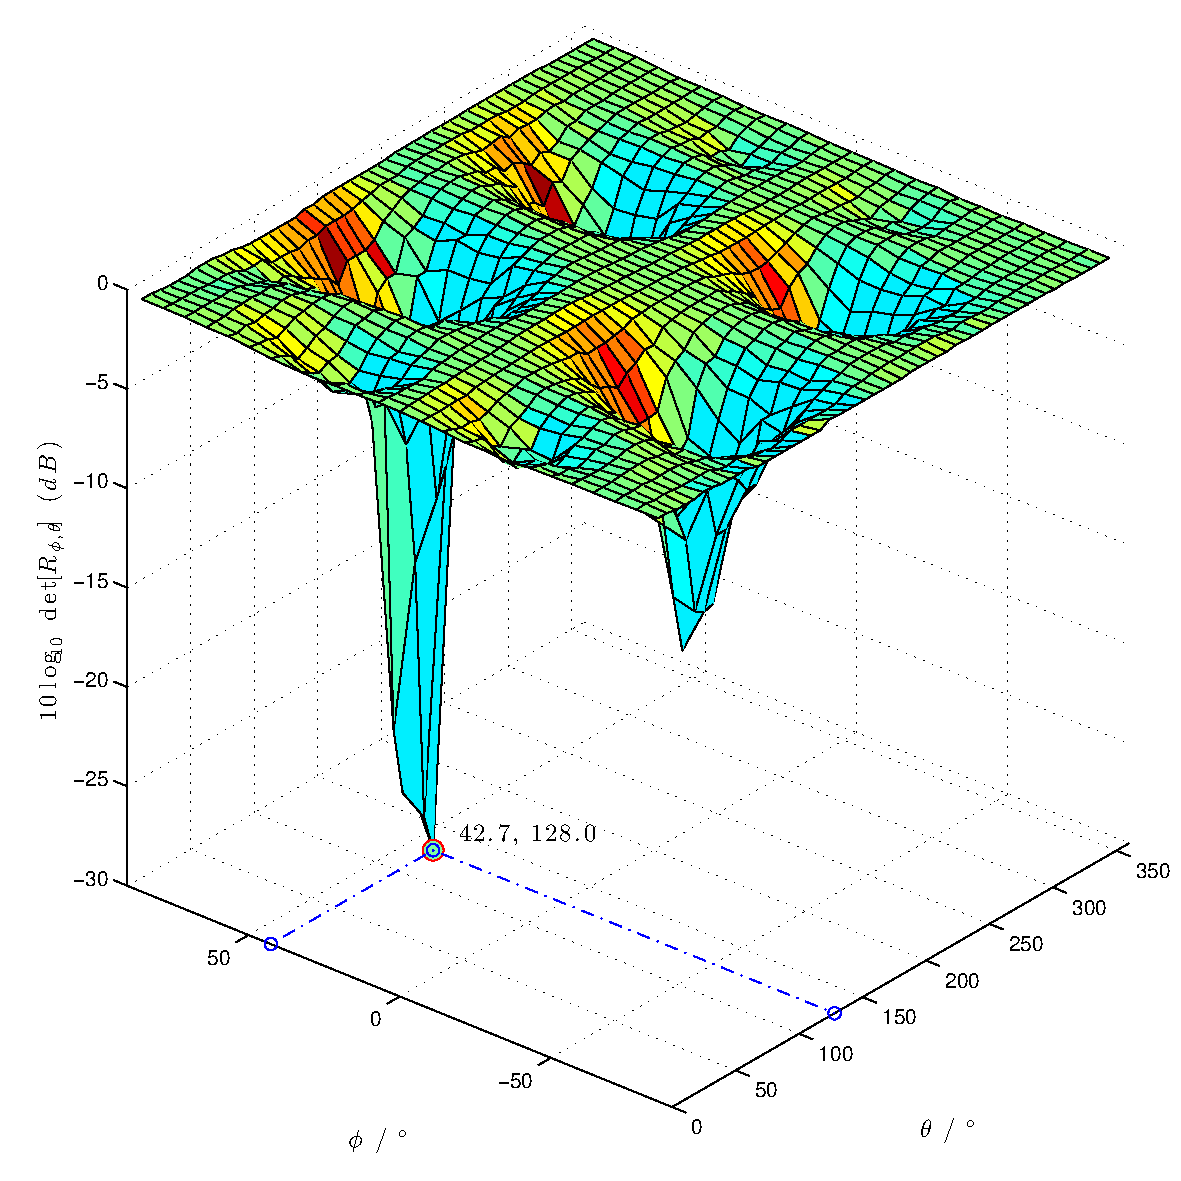
\includegraphics[width=\textwidth]{images/02_Konzeptionierung/Sim_sine_f_2000_Phi_45_Theta_120_dB_SNR_100dB}
                \caption{$f=2000Hz$}
                \label{fig:Sim_sine_f_2000_Phi_45_Theta_120_dB_SNR_100dB}
        \end{subfigure}
        ~ %add desired spacing between images, e. g. ~, \quad, \qquad etc.
          %(or a blank line to force the subfigure onto a new line)
        \begin{subfigure}[b]{0.48\textwidth}
                \centering
                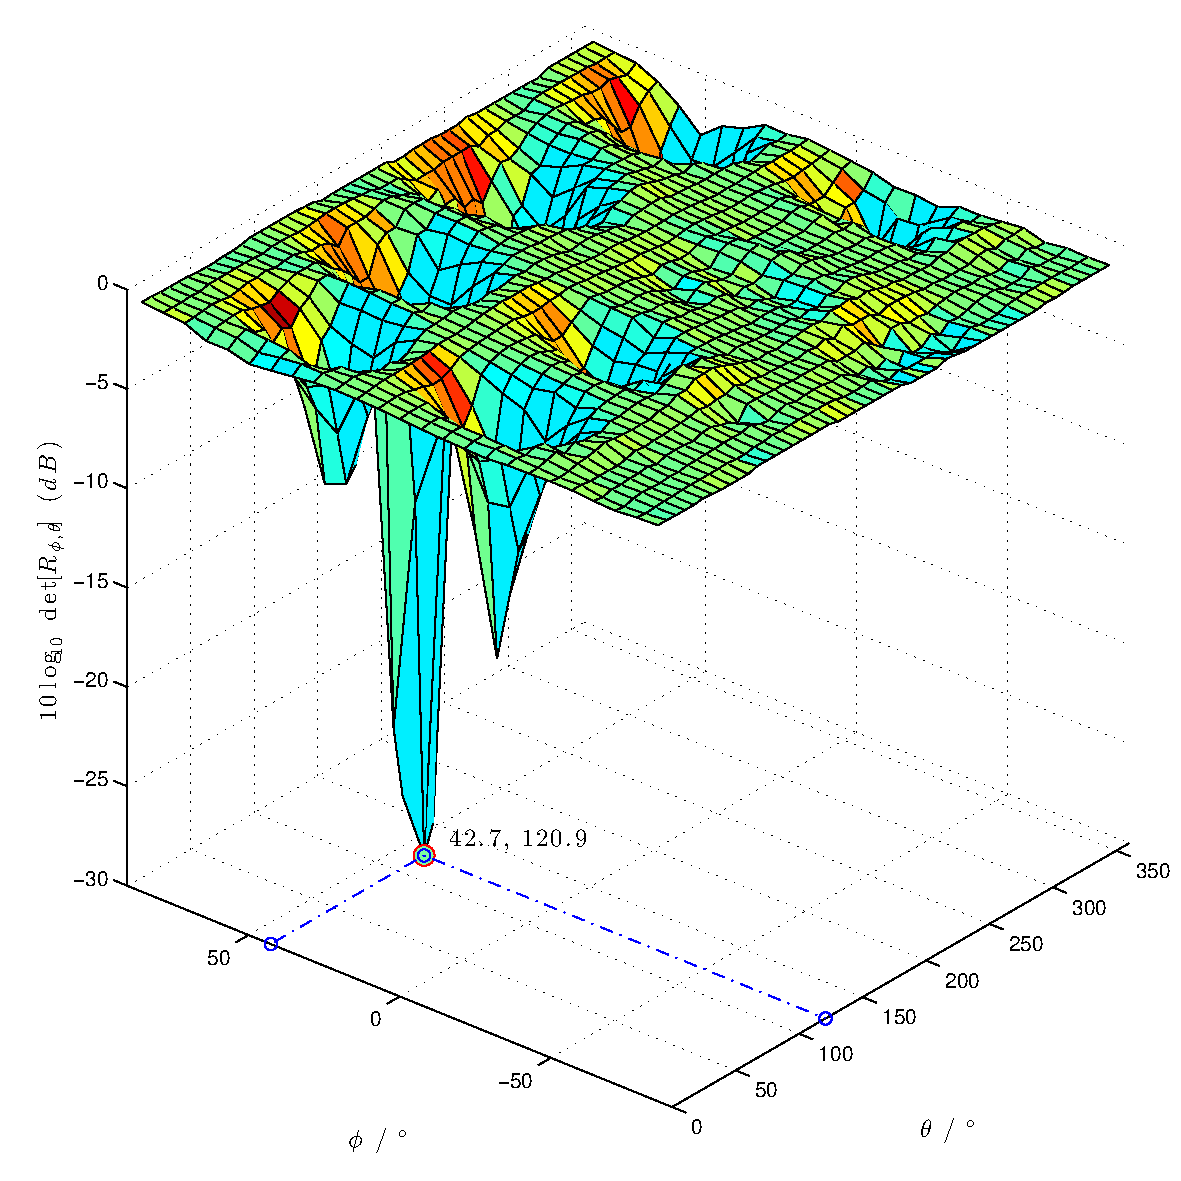
\includegraphics[width=\textwidth]{images/02_Konzeptionierung/Sim_sine_f_3000_Phi_45_Theta_120_dB_SNR_100dB}
                \caption{$f=3000Hz$}
                \label{fig:Sim_sine_f_3000_Phi_45_Theta_120_dB_SNR_100dB}
        \end{subfigure}
        \caption{Ergebnis des MCCC unter Verwendung eines synthetisch verzögerten periodischen Signals der Form $y(n) = \sin{\left( 2 \pi \frac{f}{f_a} n \right)}$ bei einer Abtastfrequenz von $f_a=48kHz$.}
        \label{fig:Sim_sine_spartial_aliasing}
\end{figure}
% ----------------------------------------- SUB-FIGURE -----------------------------------        
    


 % ****************************************************************************************
\subsubsection{Bewegte Sprachquelle} 
% ****************************************************************************************
Um das Verhalten des Systems auf eine sich durch den Raum bewegende Sprachquelle zu untersuchen, werden synthetischs Signale aus zwei folgendenSignaltypen erstellt:

\begin{itemize}
    \item bandbegrenztes weißes Rauschen
    \item Sprache (männlich und weiblich)
\end{itemize}

Folgende Simulationsparameter wurden verwendet:

\begin{itemize}
    \item Anzahl der Mikrofone $N=8$
    \item Abtastfrequenz $f_a = 44,1kHz$
    \item Signalblocklänge $L=256$ (Frame)
    \item FFT-Länge $K = 2 \cdot L = 512$
    \item Winkelauflösung $\alpha_{\phi, \theta} = 7,7°$ 
\end{itemize}

\abb{sim_diag_3D} zeigt einen künstlichen reflexionsfreien Raum mit den Abmaßen $5m \times 5m \times 3m$, in dessen Zentrum das Mikrofonarray positioniert ist. Die Rauschquelle bewegt sich hier diagonal und nimmt dabei Winkel im Bereich von $-90° \leq \phi \leq 90°$ und $\theta \in \{45°,225°\}$ an. In diesem Versuch werden zunächst die vier Eckpunkte platziert und anschließend mit einer Anzahl von 81 Stützstellen linear interpoliert. Die Rauschquelle bewegt sich somit entlang der Stützstellen um eine kleine Winkelschrittweite zu realisieren. \abb{sim_noise_diag} zeigt das Ergebnis dieses Simulationsdurchlaufs. Die in rot abgebildete Linie stellt den Fehler zu den tatsächlich eingenommene Winkeln dar. Alle Signalblöcke mit einer Blockenergie von weniger als der eingezeichneten Schwelle werden mit einem Wert $0°$ detektiert. Da wie bereits erwähnt nur diskrete Werte eingenommen werden können ist ein Fehler von $\pm \frac{\alpha_{\phi, \theta}}{2}$ zu tolerieren. Beim Betrachten des Azimuthwinkelverlaufs fällt auf, dass an den Stellen, an denen der Elevationswinkel $\phi=90°$ einnimmt ein plötzlicher Fehleranstieg stattfindet. Der Grund hierfür ist, dass sich die Quelle genau im oberen Winkeltotpunkt befindet und eine Drehung auf den Azimuthwinkel nicht erkannt werden kann. 




\myFigure{real}                                                   % Figure tag (missing, real)
         {big}                                                       % Size (small,medium,big)
         {h!}                                                  % z.B. htbp
         {Wegstrecke einer Rauschquelle  die sich diagonal durch den Raum bewegt}    % Figure title
         {sim_diag_3D}                                               % Figure label 
         {02_Konzeptionierung/sim_diag_3D}  




\myFigure{real}                                                   % Figure tag (missing, real)
         {max}                                                       % Size (small,medium,big)
         {h!}                                                  % z.B. htbp
         {Simulationsergebnis einer Rauschquelle  bei einer Blockenergieschwelle von -10dB.}    % Figure title
         {sim_noise_diag}                                               % Figure label 
         {02_Konzeptionierung/sim_noise_diag_errorbar}   



Im Folgenden soll nun eine bewegte Sprachquelle simuliert werden. Wie in \abb{sim_zig_zag_3D} dargestellt, bewegt sie sich sägezahnförmig um das Mikrofonarray und nimmt dabei Winkel im Bereich von $-45° \leq \phi \leq 45°$ und $0° \leq \theta < 360°$ an. Als Grundlage wird eine Audiodatei der Länge $T_{file}=16s$ verwendet. Bei einem zurückgelegten Weg von $s=28,9m$ beträgt die Durchschnittsgeschwindigkeit der Quelle $v=\frac{s}{T_{file}} = 6,5 \frac{km}{h}$ was der allgemeinen Angabe zur Schrittgeschwindigkeit nahe kommt.
\abb{sim_male_zig_zag} und \abb{sim_female_zig_zag} illustrieren die Ergebnisse der beiden Simulationsdurchläufe. Zu beachten ist, dass die Signale synthetisch mit dem in \Sec{subsec:ErstellungSynthetischerSignale} beschriebenen Verfahren (ohne Reflexion) blockweise verzögert werden. Die Phasenverschiebung zwischen den Kanälen ändert sich somit sprunghaft und nicht kontinuierlich wie in realer Umgebung. Die fehlerhaft erkannten Winkel (Winkelsprünge) sind zum großen Teil auf diese plötzliche Phasenänderung zurückzuführen. Die in rot abgebildete Linie stellt die Referenz zu den tatsächlich eingenommenen Winkeln dar. Alle Signalblöcke mit einer Blockenergie von weniger als der in rot dargestellten Schwelle werden mit dem Wert $0°$ detektiert. Beim Vergleich der beiden Ergebnisse zeigt sich, dass  die Zuverlässigkeit der Winkelerkennung deutlich voneinander abweicht. Dies lässt sich zum einen durch das unterschiedliche Frequenzspektrum zwischen männlicher und weiblicher Sprache begründen, zum anderen liegt eine große Differenz im Dynamikbereich\footnote{Bereich zwischen größter und kleinster Signalstärke} vor. Im Vergleich zur weiblichen Sprecherin ist der männliche etwa doppelt so groß. Die Blockenergieschwelle wird für die Simulation abhängig vom Dynamikbereich etwa in dessen Mittel gelegt. Die Ergebnisse erweisen sich trotz gelegentlicher Winkelsprünge als zufriedenstellend da die Bewegung der Quelle gut verfolgbar ist.



\myFigure{real}                                                   % Figure tag (missing, real)
         {big}                                                       % Size (small,medium,big)
         {h!}                                                  % z.B. htbp
         {Wegstrecke einer männlichen Sprechquelle die sich Zig-Zag-förmig von Position 1 bis 9 um das Mikrofonarray bewegt.}    % Figure title
         {sim_zig_zag_3D}                                               % Figure label 
         {02_Konzeptionierung/sim_zig_zag_3D}    




\myFigure{real}                                                   % Figure tag (missing, real)
         {max}                                                       % Size (small,medium,big)
         {h!}                                                  % z.B. htbp
         {Simulationsergebnis eines bewegten männlichen Sprechers (deutschsprachig) bei einer Blockenergieschwelle von -30dB.}    % Figure title
         {sim_male_zig_zag}                                               % Figure label 
         {02_Konzeptionierung/sim_male_zig_zag}    


\myFigure{real}                                                   % Figure tag (missing, real)
         {max}                                                       % Size (small,medium,big)
         {h!}                                                  % z.B. htbp
         {Simulationsergebnis eines bewegten weiblichen Sprechers (englischsprachig) bei einer Blockenergieschwelle von -20dB.}    % Figure title
         {sim_female_zig_zag}                                               % Figure label 
         {02_Konzeptionierung/sim_female_zig_zag}    







%\subsubsection{Reale Signale}





                  
% ****************************************************************************************         
\subsection{Optimierungsverfahren}
\label{subsec:Optimierungsverfahren}
% ****************************************************************************************
Im Hinblick auf die spätere Echtzeitimplementierung auf einem DSP gilt es, den Rechenaufwand so gering wie möglich zu halten. Auf Grund dessen wird ein Verfahren zur Optimierung der Suchgeschwindigkeit entwickelt. Als zweiter Optimierungsschritt folgt eine Histogrammschätzung der Richtungsergebnisse. Dieser vermindert den Effekt der abrupten Winkelsprünge. 

% ****************************************************************************************
\subsubsection{Suchgeschwindigkeit}
\label{subsubsec:Suchgeschwindigkeit}
% ****************************************************************************************
Zur Verbesserung der Suchgeschwindigkeit wird eine Methode entwickelt, die sich mit Hilfe von variablen Schrittweiten sukzessive an den korrekten Winkel annähert. \abb{prinzip_opt_suchgeschwindigkeit} zeigt das zu Grunde liegende Prinzip. Der abzusuchende Winkelbereich wird zunächst in drei Gebiete geteilt. Nun wird an den Bereichsübergängen nach dem Minimum in der räumlichen Korrelationsmatrix $R_{\phi, \theta}$ gesucht. Der gefundenen Winkel wird in der nächsten Itteration als neuer Starpunkt gewählt. Anschließend erfolgt eine Halbierung des Suchbereiches und der Vorgang beginnt erneut. Dieser Algorithmus wird so lange wiederholt, bis die minimale Schrittweite erreicht wurde. 

\myFigure{real}                                                   % Figure tag (missing, real)
         {medium}                                                       % Size (small,medium,big)
         {h!}                                                  % z.B. htbp
         {Methode zur Optimierung der Suchgeschwindigkeit mit Hilfe einer variablen Schrittweiten.}    % Figure title
         {prinzip_opt_suchgeschwindigkeit}                                               % Figure label 
         {02_Konzeptionierung/prinzip_opt_suchgeschwindigkeit} 


% ****************************************************************************************
\subsubsection{Histogramm}
\label{subsubsec:Histogramm}
% ****************************************************************************************
Zur Reduktion der Winkelsprünge bei \zB überlagerten Störungen wird im Folgenden eine Histogrammschätzung durchgeführt. Die detektierten Winkel werden im laufenden Betrieb kontinuierlich in einen Ringspeicher mit einer variabel einstellbaren Länge gespeichert. Nach jedem Suchvorgang erfolgt eine Häufigkeitsanalyse des Ringspeicherinhalts. \abb{sim_female_zig_zag_dist_sample_frame_864} zeigt illustriert ein Beispiel für die Häufigkeitsanalyse des weiblichen Sprachsignals mit einer Ringspeicherlänge von 50 Werten sowie einer Häufigkeitsschwelle von 20\%. Tritt ein gemessener Winkel so häufig auf, dass er diese Schwelle überschreitet wird er als wahrscheinlich genug eingestuft und als gültig markiert. Tritt der Fall ein, dass die Häufigkeit keines Ringspeicherwerts diese Schwelle überschreitet, markiert der Algorithmus den aktuellen Signalblock als ungültig.



\abb{sim_male_female_zig_zag_hist_comp} und \abb{sim_male_zig_zag_hist_comp} zeigen einen Vergleich der Simmulationsergebnisse des männlichen und weiblichen Sprechers mit und ohne Histogrammoptimierung. Es ist deutlich zu sehen, dass abrupte Winkelsprünge nahezu verschwiden. Bei solch einem Verfahren, das Ergebniswerte zwischenspeichert, tritt eine Verzögerung auf, die abhängig von der Ringspeicherlänge sowie der eben erwähnten Schwelle ist. Im Vergleich zum nicht optimierten Ergebnis ist das optimierte leicht zur Winkelreferenzkurve verschoben.


\myFigure{real}                                                   % Figure tag (missing, real)
         {medium}                                                       % Size (small,medium,big)
         {h!}                                                  % z.B. htbp
         {Histogramm eines bewegten weiblichen Sprechers}    % Figure title
         {sim_female_zig_zag_dist_sample_frame_864}                                               % Figure label 
         {02_Konzeptionierung/sim_female_zig_zag_dist_sample_frame_864} 


\myFigure{real}                                                   % Figure tag (missing, real)
         {max}                                                       % Size (small,medium,big)
         {h!}                                                  % z.B. htbp
         {Vergleich zwischen Winkelverlauf mit und ohne Histogrammschätzung beim weiblichen Sprecher mit einer Ringspeicherlänge von 50 und einer Schwelle von 15\%}    % Figure title
         {sim_male_female_zig_zag_hist_comp}                                               % Figure label 
         {02_Konzeptionierung/sim_female_zig_zag_hist_comp} 


\myFigure{real}                                                   % Figure tag (missing, real)
         {max}                                                       % Size (small,medium,big)
         {h!}                                                  % z.B. htbp
         {Vergleich zwischen Winkelverlauf mit und ohne Histogrammschätzung beim männlichen Sprecher mit einer Ringspeicherlänge von 50 und einer Schwelle von 15\%}    % Figure title
         {sim_male_zig_zag_hist_comp}                                               % Figure label 
         {02_Konzeptionierung/sim_male_zig_zag_hist_comp} 






